\documentclass[11pt,a4paper,oneside]{book} %scrbook book report

\usepackage[
backend=biber,
style=apa,
sorting=nyt
]{biblatex}
\addbibresource{references.bib}

% Essential packages
\usepackage{amsmath, amssymb, amsthm} % AMS Packages
\usepackage{graphicx,color}           % Packages for graphics and color
\usepackage[left=1.25in, right=1.25in, top=1in, bottom=1in, includefoot, headheight=13.6pt]{geometry}
\PassOptionsToPackage{printonlyused,smaller}{acronym}
\usepackage{acronym}
% Optional customization packages
\usepackage{lmodern}                  % Custom fonts
\usepackage[T1]{fontenc}              % Ensure correct font encoding
\usepackage{mathptmx}              % Times New Roman Font accross the document
\usepackage{ragged2e}
\usepackage{url}

% Customising chapter headings - sectsty.pdf
\usepackage{sectsty}
\chapterfont{\Large\sc\centering}
\chaptertitlefont{\centering}
\subsubsectionfont{\centering}

\usepackage[hang, small, bf, margin=0pt, tableposition=bottom]{caption}
\setlength{\abovecaptionskip}{10pt}   % Custom captions

% Tables
\usepackage[table]{xcolor}
\usepackage{colortbl}

\newcommand{\mc}[2]{\multicolumn{#1}{c}{#2}}
\definecolor{Gray}{gray}{0.83}

\newcolumntype{x}{>{\columncolor{Gray}}c}
\newcolumntype{y}{>{\columncolor{white}}c}

% Page layout
\parindent 0pt
\parskip 1ex
\renewcommand{\baselinestretch}{1.49}
\numberwithin{equation}{section}
\renewcommand{\bibname}{References}
\renewcommand{\contentsname}{Contents}
\pagenumbering{roman}


\newcommand{\acrolabel}[1]{\makebox[3cm][l]{\textbf{#1}}}
\newenvironment{acronyms}{\begin{list}{}{\renewcommand{\makelabel}{\acrolabel}}}{\end{list}}

% Customising headers - fancyhdr.pdf
\usepackage{fancyhdr}
\pagestyle{fancy}
\rhead{}
\lhead{\nouppercase{\textsc{\leftmark}}}
\renewcommand{\headrulewidth}{0pt}
\makeatletter
\renewcommand{\chaptermark}[1]{\markboth{\textsc{\@chapapp}\ \thechapter:\ #1}{}}
\makeatother


% Hyperreferencing and citations
\usepackage{hyperref}
\hypersetup{
    colorlinks,
    citecolor=blue,
    filecolor=blue,
    linkcolor=blue,
    urlcolor=blue
}

% Section symbol
\usepackage{cleveref}
\crefname{section}{\S}{\S\S}
\Crefname{section}{\S}{\S\S}
\crefname{subsection}{\S}{\S\S}
\Crefname{subsection}{\S}{\S\S}


\usepackage{adjustbox}
\usepackage{booktabs}% for better rules in the table
\usepackage{array}
\usepackage{seqsplit}
\usepackage{graphicx}
\usepackage{./styles/astron}
\usepackage{./styles/gcuf}
\graphicspath{{./img/}{./figs/}}

\title{An Agentic Large Language Model Assistant for Kaggle Computational Notebooks}
\subtitle{A Chrome Extension and Python Native Host with DOM-Grounded Context and Tool-Mediated Cell Operations}

\authorone{Hamza Ali}
\authortwo{Muhammad Zubair}
\regnoone{2022-GCUF-02772}
\regnotwo{2022-GCUF-02760}
\degree{\BSDS} % BSDS, BSDA %% Degree Title and It's abbreviation
\dept{\CDS} %Dept abbreviation and Full Name

\supervisor{Rabia Shahid}
\supervisorAffiliation{Center of Data Science}

\date{June 2026}

\begin{document}
\maketitle
\chapter*{Center of Data Science}

    \centering
    
\includegraphics[width=0.30\textwidth]{img/dslogo.png}
    
   
\justifying
The Center of Data Science (CDS) at Government College University Faisalabad (GCUF) is a forward-looking academic and research hub committed to advancing data-driven education, innovation, and societal impact. Guided by a clear vision to produce globally competitive data scientists and knowledge leaders, the Center plays a vital role in addressing real-world challenges through analytics, artificial intelligence, and emerging digital technologies. Equipped with modern infrastructure, state-of-the-art computing facilities, and advanced research laboratories, CDS provides an enabling environment for learning, experimentation, and innovation. The Center is supported by a team of highly qualified and experienced faculty, actively engaged in teaching, research, and industry collaboration. With a strong emphasis on market-based research, CDS fosters the development of practical solutions, intelligent applications, and data-driven products that add tangible value to society, contribute to economic growth, and support evidence-based decision-making across academia, industry, and the public sector.
    
\chapter*{Approval}
It is certified that the contents and form of the FYP/thesis entitled ``\textbf{\fyptitle}" submitted by \textbf{Hamza Ali and Muhammad Zubair} have been found satisfactory for the requirement of the degree.

\vspace*{\stretch{1}}
\vspace*{10pt}\noindent
Supervisor: \textbf{\underline{\fypsupervisor}}\vspace*{10pt}\noindent\\
Signature: \line(1,0){100}\vspace*{10pt}\noindent\\
\vspace*{10pt}\noindent
Date:  \line(1,0){100}

\vspace*{\stretch{1}}

\begin{flushright}
Committee Member 1: \textbf{\underline{Dr.\ Adeel Zahid}}\\
\vspace*{10pt}\noindent
Signature: \line(1,0){100}\\
\vspace*{10pt}\noindent
Date:  \line(1,0){100}

\vspace*{\stretch{1}}

Committee Member 2: \textbf{\underline{Khuram Shahzad}}\\
\vspace*{10pt}\noindent
Signature: \line(1,0){100}\\
\vspace*{10pt}\noindent
Date:  \line(1,0){100}

\vspace*{\stretch{1}}

Head of Department: \textbf{\underline{Prof.\ Dr.\ Tanvir Ahmad}}\\
\vspace*{10pt}\noindent
Signature: \line(1,0){100}\\
\vspace*{10pt}\noindent
Date:  \line(1,0){100}
\end{flushright}

\chapter*{FYP/Thesis Acceptance Certificate}

Certified that final copy of BSDS/DA/MS/MPhil thesis entitled ``\textbf{\@title}" written by \textbf{\@author}, (Registration No \textbf{\@regno}), of \@dept has been vetted by the undersigned, found complete in all respects as per GCUF Statutes/Regulations, is free of plagiarism, errors and mistakes and is accepted as partial fulfillment for award of MS/M Phil degree. It is further certified that necessary amendments as pointed out by FYP/Thesis  Evaluation members of the scholar have also been incorporated in the said FYP/thesis.
        
    \begin{flushright}
    \vspace*{\stretch{2}}
    Signature: \line(1,0){100}\\
    \vspace*{10pt}\noindent
    Name of Advisor: \textbf{\underline{\@supervisor}}\\
    \vspace*{10pt}\noindent
    Date: \line(1,0){100}
    
    \vspace*{\stretch{2}}
    Signature (Member1): \line(1,0){100}\\
    \vspace*{10pt}\noindent
    Date:  \line(1,0){100}
     \vspace*{\stretch{2}}
    \\ Signature (Member2): \line(1,0){100}\\
    \vspace*{10pt}\noindent
    Date:  \line(1,0){100}

    \vspace*{\stretch{1}}
    Signature (Director): \line(1,0){100}\\
    \vspace*{10pt}\noindent
    Date:  \line(1,0){100}
    \vspace*{\stretch{1}}
    \end{flushright}
\chapter*{Dedication}
This FYP/thesis is dedicated to all the deserving children who do not have access to quality education especially young girls.
\chapter*{Certificate of Originality}
I hereby declare that this submission is my own work and to the best of my knowledge it contains no materials previously published or written by another person, nor material which to a substantial extent has been accepted for the award of any degree or diploma at \fypsupervisoraffiliation\ at \fypdept\ or at any other educational institute, except where due acknowledgement has been made in the FYP. Any contribution made to the research by others, with whom I have worked at \fypdept\ or elsewhere, is explicitly acknowledged in the FYP. I also declare that the intellectual content of this FYP is the product of my own work, except for the assistance from others in the project's design and conception or in style, presentation and linguistics which has been acknowledged.
\vspace*{10pt}\noindent
\begin{flushright}
Student Name: \textbf{\underline{Hamza Ali}}\\
\vspace*{10pt}\noindent
Signature: \line(1,0){100}\\
\vspace*{14pt}\noindent
Student Name: \textbf{\underline{Muhammad Zubair}}\\
\vspace*{10pt}\noindent
Signature: \line(1,0){100}
\end{flushright}


\chapter*{Acknowledgments}
Glory be to Allah (S.W.A), the Creator, the Sustainer of the Universe. Who only has the power to honour whom He please, and to abase whom He please. Verily no one can do anything without His will. From the day, I came to GCUF till the day of my departure, He was the only one Who blessed me and opened ways for me, and showed me the path of success. Their is nothing which can payback for His bounties throughout my research period to complete it successfully.
\vspace*{\stretch{1}}

\begin{flushright}
\textbf{\underline{\@author}}
\end{flushright}

\chapter*{Abstract}
\vspace{-\baselineskip}
\noindent Computational notebooks support data science learning, yet practical assistance inside browser-based editors remains limited. Code assistants optimised for file-based repositories poorly serve Kaggle notebooks, where work proceeds through indexed cells in a dynamic web interface. This Final Year Project presents an agentic large language model assistant for Kaggle computational notebooks, implemented as a Chrome extension with a Python native host. The system captures notebook context via DOM-grounded scraping, maintains live and persistent JSON snapshots, and exposes tool-mediated cell insertion, editing, deletion, and execution. Three interaction modes---Ask, Code, and Agentic---enforce distinct contracts: read-only explanation, copy-paste code with placement guidance, and batched tool dispatch under a mandatory two-phase protocol. The host validates tool arguments, coerces session metadata, and applies deterministic ordering for index-sensitive multi-cell operations. Empirical evaluation on frozen Kaggle snapshots using GLM~4.7 reports Ask mode achieving 89\% workflow topic coverage with zero side effects and reliable cell-level explanation and error diagnosis; Code mode passing four scenarios with runnable Python cells and zero browser writes. The prototype demonstrates that effective in-browser notebook assistance is feasible without privileged platform APIs through constrained tool orchestration and grounded context extraction, contributing a practical blueprint for safe LLM-assisted workflows in web-native notebook environments.

\vspace{1.5ex}
\noindent\textbf{Keywords:} Computational notebooks, large language models, Kaggle notebooks, Chrome extension, native messaging, DOM grounding, agentic artificial intelligence, tool calling, data science, GLM-4.7



\tableofcontents
\listoftables
\listoffigures
\chapter*{List of Abbreviations and Symbols}
\section*{Abbreviations}
\begin{acronym}[JupyterLab]
\acro{API}{Application Programming Interface}
\acro{BSDS}{Bachelor of Science in Data Science}
\acro{CDS}{Center of Data Science}
\acro{DOM}{Document Object Model}
\acro{FYP}{Final Year Project}
\acro{GCUF}{Government College University Faisalabad}
\acro{LLM}{Large Language Model}
\acro{RAG}{Retrieval-Augmented Generation}
\acro{RLHF}{Reinforcement Learning from Human Feedback}
\acro{UI}{User Interface}
\end{acronym}

% \acf{} for full description, must be used for declaration, when using/define acronym for the first time
% \ac{} to be used when abbreviation is required only for reference.

\resetpagenumbering

%!TEX root = ../_fyp-ch1-preview.tex
\chapter{Introduction and Motivation}
\label{c-intro}

Computational notebooks have become a primary medium for data science education, experimentation, and competition-oriented analytics. Platforms such as Kaggle expose browser-based notebook editors in which analysts interleave narrative markdown, executable code, and model outputs within a single document. The resulting workflow is iterative: cells are authored, reordered, executed, and revised as understanding of the data evolves. For novice and intermediate practitioners, this cycle demands fluency in both domain reasoning and editor mechanics, yet mainstream assistance remains largely decoupled from the live notebook surface.

Recent advances in large language models (\acp{LLM}) have produced capable coding assistants that answer questions, suggest snippets, and generate multi-step solutions from natural-language prompts. However, when the task environment is a proprietary web editor rather than a local integrated development environment, assistants typically operate on pasted fragments or static file exports. They cannot reliably observe cell order, execution state, or structural changes that occur as the user edits in real time. Consequently, suggestions may reference stale indices, omit required execution steps, or remain disconnected from the notebook the analyst is actually building.

This project addresses that integration gap by developing an agentic \ac{LLM} assistant tailored to Kaggle notebook \texttt{/edit} pages. The system couples a Chrome extension with a Python native messaging host. The extension scrapes the editor \ac{DOM} to maintain live and persistent JSON snapshots of notebook structure and cell content. The host mediates chat in Ask, Code, and Agentic modes, invokes a GLM~4.7 model with native \texttt{tool\_calls} via the Cerebras \ac{API}, and dispatches browser-mediated tools that insert, edit, delete, list, and run cells. Session context is grounded in the scraped notebook state and coerced to the active tab URL, yielding an in-browser copilot that manipulates the notebook the user sees rather than a detached code buffer.

The remainder of this document specifies the problem the assistant is designed to solve, states the research objectives and aims, summarises original contributions, and acknowledges scope limitations. A full literature review follows in the next chapter; here we establish motivation and the precise gap this work targets.

\section{Problem Statement and Contribution}
\label{sec:problem-statement}

Despite widespread adoption of \ac{LLM}-powered coding tools, no widely available assistant provides deep, tool-mediated integration with the Kaggle notebook editor running inside Chrome. General-purpose chat interfaces and IDE extensions assume access to repository files or user-supplied excerpts. They do not maintain a continuously updated representation of notebook cells as rendered in the browser, nor do they execute a constrained repertoire of editor operations with deterministic ordering guarantees. On Kaggle, cell identity is positional rather than stable: inserts and deletes shift indices, so batch modifications require careful sequencing. Existing assistants rarely enforce a read-then-write discipline, cap model rounds to control latency and cost, or reconcile bulk operations on the host before dispatch to the extension.

The central problem addressed by this FYP is therefore twofold. First, \emph{context grounding}: how to extract faithful, timely notebook structure and content from a closed web application without privileged \ac{API} access, and how to supply that context to an \ac{LLM} during interactive assistance. Second, \emph{reliable agentic manipulation}: how to translate model-proposed tool calls into safe, ordered sequences of DOM-level cell operations---including multi-cell insert--edit--run workflows---while binding each action to the correct browser tab and notebook session.

Answering this problem is worthwhile because Kaggle notebooks are a high-stakes learning and competition environment for data science students, including those in the \acf{BSDS} programme at \acf{CDS}, \acf{GCUF}. In-browser assistance that reads the live notebook and applies vetted tools can reduce friction in exploratory analysis, support reproducible cell-level edits, and demonstrate a reusable architecture for DOM-grounded agentic systems where platform \acp{API} are unavailable. The approach also informs design choices for future notebook copilots that must balance model autonomy with strict execution contracts.

\subsection{Aims}
\label{sec:aims}

The overarching aim of this project is to design, implement, and evaluate an agentic \ac{LLM} assistant that operates directly on Kaggle computational notebooks within Google Chrome. Specifically, the work aims to:

\begin{itemize}
  \item provide conversational assistance grounded in scraped notebook state rather than user-copied code alone;
  \item expose a bounded tool interface through which the model can inspect and modify cells in the live editor;
  \item enforce predictable agentic behaviour through a mandatory two-phase query--implement protocol and host-side batch reordering; and
  \item demonstrate feasibility on representative Kaggle \texttt{/edit} sessions relevant to data science coursework and competition workflows.
\end{itemize}

\subsection{Research Objectives}
\label{sec:objectives}

The following research objectives guide the design and evaluation of the system:

\begin{enumerate}
  \item \textbf{Architecture.} Specify and implement a Chrome extension and Python native messaging host that communicate securely, route chat by mode (Ask, Code, Agentic), and associate each request with the active notebook URL and browser tab identifier.
  \item \textbf{Context pipeline.} Develop a DOM-scraping pipeline that serialises notebook cells into live and persistent JSON snapshots, enabling the host to inject current structure and content into \ac{LLM} prompts without manual copy-and-paste.
  \item \textbf{Tool-mediated cell operations.} Implement and register browser tools with session URL and \texttt{tab\_id} coercion so dispatches target the correct editor instance. Mutation tools are \texttt{insert\_cell}, \texttt{edit\_cell\_by\_index}, \texttt{delete\_by\_index}, and \texttt{run\_cell}. Read tools are \texttt{notebook\_get\_cell} and \texttt{list\_cells}.
  \item \textbf{Agentic execution contract.} Integrate GLM~4.7 native \texttt{tool\_calls} (Cerebras) under a mandatory two-phase protocol (read-only query, then implement), a maximum of two \ac{API} calls per user message, fire-and-forget batch dispatch, and host-side descending reorder for bulk delete and insert operations.
  \item \textbf{Run and structure detection.} Use scrape-based monitors rather than WebSocket access to infer cell execution and notebook structure changes, supporting operational feedback within platform constraints.
  \item \textbf{Empirical validation.} Exercise the assistant on Kaggle notebook editing scenarios---including multi-cell workflows---and assess whether DOM-grounded context and ordered tool batches produce coherent, session-consistent modifications.
\end{enumerate}

\subsection{Original Contributions}
\label{sec:contributions}

This FYP makes the following original contributions:

\begin{itemize}
  \item A \textbf{split extension--host architecture} for Kaggle notebook assistance, separating in-browser DOM interaction from \ac{LLM} orchestration, snapshot persistence, and tool dispatch on the native host.
  \item A \textbf{DOM-grounded context pipeline} that maintains live and persistent JSON notebook snapshots derived from editor scraping, supplying the model with positional cell labels and content aligned to the user's current session.
  \item A \textbf{bounded agentic execution model} comprising a mandatory two-phase query--implement cycle, a hard limit of two model calls per user turn, and fire-and-forget batch execution with explicit tool ordering (deletes before inserts, runs last).
  \item \textbf{Host-side index reconciliation} that reorders bulk delete and insert tool calls in descending index order to reduce index-shift errors during multi-cell modifications.
  \item \textbf{Session binding mechanisms} that coerce notebook URL and \texttt{tab\_id} across tool arguments, mitigating mismatches when the model omits or approximates session metadata.
  \item \textbf{Scrape-based operational monitoring} for cell runs and structural change detection in the absence of a documented Kaggle editor automation \ac{API}.
\end{itemize}

\subsection{Limitations}
\label{sec:limitations}

The scope of this work is deliberately constrained. The assistant targets \textbf{Kaggle notebook \texttt{/edit} pages only}; other notebook platforms, local JupyterLab instances, and non-edit Kaggle views are out of scope. Deployment is \textbf{Chrome-specific}, relying on extension APIs and native messaging unavailable in all browsers. Agentic mode employs \textbf{fire-and-forget dispatch} without a full host-driven verification or recovery loop: the model must complete read and write phases within two calls, and execution outcomes are surfaced through monitors rather than closed-loop replanning. \textbf{\ac{LLM} \ac{API} limits}---latency, rate limits, and model behaviour---affect responsiveness and tool-call reliability. \textbf{DOM scraping} introduces sensitivity to front-end layout changes and incurs observational delay compared with privileged editor hooks. Finally, \textbf{execution metadata} (e.g., rich stderr traces, variable-level runtime state) is not yet fed back comprehensively to the model; a systematic verification loop remains identified future work, as discussed in later chapters.

\section{Background and Context}
\label{sec:background}

\subsection{Computational notebooks in data science education}

Computational notebooks occupy a central role in contemporary data science curricula \parencite{kluyver2016jupyter,perez2007ipython}. At \acf{GCUF}, the \acf{BSDS} programme introduces students to exploratory data analysis, statistical modelling, and machine-learning workflows through hands-on notebook exercises. Unlike traditional software projects organised as scripts or packages, notebook assignments emphasise \emph{narrative reproducibility}: each analytical step is visible as a cell, outputs appear inline, and markdown cells document reasoning for instructors and peers \parencite{rule2019tenrules}.

Kaggle extends this pedagogical model into a public competition and portfolio platform. Learners fork existing kernels, adapt feature-engineering pipelines, and publish notebooks that combine code, visualisation, and commentary \parencite{quaranta2021kgtorrent,wang2021welldocumented}. The platform's browser editor, however, does not expose a documented automation \ac{API} to third-party assistants. Students therefore rely on manual cell editing, copy-paste from external chat tools, or platform-native features that lack deep language-model integration \parencite{mcnutt2023notebookassistants}.

\subsection{The assistance gap on closed web editors}

Mainstream coding assistants---including GitHub Copilot and general-purpose chat interfaces---were designed for file-centric development environments \parencite{ziegler2024copilot,chen2021codex}. When a student works inside Kaggle's \texttt{/edit} view, several properties diverge from that assumption:

\begin{itemize}
  \item \textbf{Positional cell identity.} Cells are referenced by index; inserts and deletes shift subsequent positions.
  \item \textbf{Mixed modalities.} Markdown and code cells interleave; assistance must respect cell type.
  \item \textbf{Execution coupling.} Code meaning depends on prior kernel state not visible in a static export.
  \item \textbf{Session binding.} Multiple notebook tabs may be open; actions must target the correct editor instance.
  \item \textbf{Platform closure.} No privileged hooks exist for external agents to list, edit, or run cells programmatically.
\end{itemize}

These properties motivate a client--host architecture that scrapes the live \ac{DOM}, persists JSON snapshots, and dispatches vetted tools rather than treating the notebook as a single text buffer \parencite{chasins2018roussillon,lewis2020rag}.

\subsection{Role of large language models}

Recent \acp{LLM} demonstrate strong code synthesis and explanation capabilities \parencite{brown2020language,chen2021codex,openai2023gpt4}. Tool-augmented variants extend this capability by invoking structured APIs during generation \parencite{schick2023toolformer,qin2024toolllm,yao2023react}. For notebook assistance, the research question is not whether a model can write pandas or scikit-learn code in isolation---benchmarks establish that baseline---but whether a \emph{deployable system} can ground each turn in the user's current notebook and, when appropriate, execute cell operations safely \parencite{hou2024llm4se,vaithilingam2022expectation}.

This FYP answers that question through a Chrome extension and Python native host that implement three deliberately separated interaction modes: Ask (explain), Code (generate for copy-paste), and Agentic (dispatch tool batches).

\section{Project Scope and Delimitations}
\label{sec:scope}

Table~\ref{tab:scope} summarises what is included and excluded from the project boundary.

\begin{table}[!ht]
\centering
\caption{Project scope and explicit delimitations.}
\label{tab:scope}
\small
\begin{tabular}{|p{3.2cm}|p{4.8cm}|p{4.8cm}|}
\hline
\textbf{Dimension} & \textbf{In scope} & \textbf{Out of scope} \\ \hline
Platform & Kaggle \texttt{/edit} in Chrome & JupyterLab, Colab, VS Code notebooks \\ \hline
Model provider & GLM~4.7 via Cerebras \ac{API} & Multi-provider orchestration \\ \hline
Agentic control & Two-call query--implement; fire-and-forget batch & Full ReAct loop with replanning \\ \hline
Evaluation & Harness benchmarks on frozen snapshots & Large-scale human subjects study \\ \hline
Deployment & Local native host + extension & Cloud-hosted SaaS assistant \\ \hline
\end{tabular}
\end{table}

Delimitations are intentional: they keep the artefact reproducible within FYP timelines while demonstrating principles transferable to other closed notebook surfaces \parencite{mcnutt2023notebookassistants}.

\section{Stakeholders and Use Cases}
\label{sec:stakeholders}

The assistant serves three stakeholder groups with distinct use cases:

\subsection{Data science students}

\acf{BSDS} students fork public Kaggle kernels for assignments and competitions. Typical tasks include understanding an unfamiliar notebook (Ask), implementing a new modelling cell without breaking upstream dependencies (Code), and batch-adding analysis sections during project work (Agentic). Mode separation lets instructors recommend Ask-only sessions during formative weeks and controlled Agentic use during capstone projects.

\subsection{Competition participants}

Kaggle competitors iterate rapidly on feature engineering and model selection under time pressure \parencite{quaranta2022bestpractices}. Code mode supports quick generation of experimental cells with placement hints; Agentic mode can plan multi-cell pipelines when the user accepts review of dispatched batches. Ask mode supports post-mortem analysis of errors in failed submissions.

\subsection{System maintainers and researchers}

Developers extending the extension--host stack need reproducible benchmarks (Appendix~\ref{app:benchmarks}) and modular prompts under \texttt{testing/host/prompts/}. Researchers studying notebook copilots can use the frozen snapshot harness to compare models without live Kaggle sessions.

Table~\ref{tab:use-cases} maps common tasks to recommended modes.

\begin{table}[!ht]
\centering
\caption{Representative use cases and recommended modes.}
\label{tab:use-cases}
\small
\begin{tabular}{|p{4.2cm}|p{2.4cm}|p{5.8cm}|}
\hline
\textbf{Task} & \textbf{Mode} & \textbf{Rationale} \\ \hline
Explain an error traceback & Ask & Zero side effects; cites cell evidence \\ \hline
Add XGBoost training cell & Code & Runnable block; user controls insert \\ \hline
Build EDA + modelling section & Agentic & Multi-cell batch after structure query \\ \hline
Clarify empty cell intent & Ask / Code & Deferral pattern; no unsolicited code \\ \hline
Review competition kernel & Ask & Workflow coverage without mutation \\ \hline
\end{tabular}
\end{table}

\section{Thesis Organisation}
\label{sec:organisation}

The remainder of this document is organised as follows. Chapter~\ref{c-review} surveys prior work on notebooks, \ac{LLM}-assisted coding, retrieval grounding, and agentic tool use. Chapter~\ref{c-methods} presents the research design, system architecture, implementation methodology, and evaluation protocol. Chapter~\ref{c-results} reports benchmark outcomes for Ask, Code, and Agentic modes. Chapter~\ref{chap:discussion} interprets findings against the literature and states threats to validity. Chapter~\ref{cha:conclusion} concludes with contributions and future work. Chapter~\ref{c-recommendation} offers recommendations for practitioners, maintainers, and researchers. Appendix~\ref{app:benchmarks} lists benchmark prompts and tool definitions for reproducibility.

%!TEX root = ../_fyp.tex
\chapter{Literature Review}
\label{c-review}

Chapter~\ref{c-intro} established that mainstream \ac{LLM} assistants remain poorly integrated with proprietary, browser-hosted notebook editors such as Kaggle. The problem couples two research threads: how analysts work in computational notebooks, and how modern language models can be grounded in live application state while executing structured tool actions. This chapter surveys prior work along those threads, organised by idea rather than chronology. We first examine notebook-centric data science practice and the Kaggle ecosystem; then review \ac{LLM} applications to code and data science; discuss retrieval-augmented and context-grounded generation; analyse agentic models that interleave reasoning with tool use; and address integration challenges for web-based notebook environments. The chapter closes by synthesising the research gap and positioning the present FYP relative to notebook assistants, IDE copilots, and platform-native tooling.

\section{Computational Notebooks and Data Science Workflows}
\label{sec:lit-notebooks}

Computational notebooks interleave executable code, narrative text, and rich outputs in a single literate document. \textcite{perez2007ipython} introduced \texttt{IPython} as an interactive shell and architecture for scientific computing in Python, emphasising a read--eval--print loop that keeps code, results, and visualisations co-located. That design philosophy matured into the Jupyter ecosystem described by \textcite{kluyver2016jupyter}, who characterised Jupyter Notebooks as a publishing format for \emph{reproducible computational workflows}. Cells can be reordered and re-executed non-linearly; markdown supports exposition; and kernel outputs embed directly beneath the code that produced them. For data science education and practice---including programmes such as the \acf{BSDS} at \acf{GCUF}---notebooks lower the barrier between exploratory analysis and communicable artefact.

Empirical studies clarify how practitioners actually use this medium. \textcite{rule2018exploration} distinguish \emph{exploration} notebooks, in which analysts iteratively probe data, from \emph{explanation} notebooks intended for presentation and reuse. The same structural affordances that support experimentation---mutable cell order, inline outputs, and narrative/code interleaving---also complicate maintenance when notebooks evolve from private sketches into shared deliverables. \textcite{rule2019tenrules} codify practical guidance for writing and sharing analyses in Jupyter, stressing clear sectioning, reproducible execution order, and documentation habits that later readers can follow without re-running every cell blindly.

Kaggle has become a prominent venue for notebook-centric data science at scale. \textcite{quaranta2021kgtorrent} released KGTorrent, a corpus of Python Jupyter notebooks harvested from Kaggle, enabling mining of structural and content patterns across thousands of public analyses. \textcite{wang2021welldocumented} studied documentation practices in Kaggle notebooks through interviews and content analysis, finding that effective notebooks balance code, markdown explanation, and visual evidence---yet many notebooks remain under-documented or difficult to reuse. \textcite{quaranta2022bestpractices} extended this line by eliciting collaborative best practices for computational notebooks and assessing their adoption in Kaggle-derived notebooks; experts recognise recommendations such as modular cell structure and explicit data provenance, but tool support and competition deadlines often impede consistent adherence.

Together, this literature establishes three properties relevant to the present project. First, notebook work is \emph{cell-oriented}: meaningful units are indexed positions containing code or markdown, not abstract symbols in a flat source file. Second, workflows are \emph{iterative and non-linear}; assistance must tolerate reordering, re-execution, and partial drafts. Third, Kaggle notebooks sit within a \emph{web platform} whose social and competitive context shapes authoring norms. Competition deadlines, public leaderboards, and fork-and-remix culture encourage rapid experimentation over polished software engineering discipline---a tension \textcite{quaranta2022bestpractices} document when recommended practices collide with time pressure.

From a systems perspective, notebooks also decouple \emph{authoring state} from \emph{execution state}. A cell may contain code that has not been run, code whose output is stale, or markdown that documents results from an earlier kernel session. Assistants that treat notebook files as static text risk proposing edits that contradict execution order or ignore hidden failures in prior cells. \textcite{rule2018exploration} note that analysts frequently pivot between exploratory and explanatory stances within the same document, interleaving throwaway diagnostics with narrative intended for peers. An effective copilot must therefore present the model with both structural layout (which cells exist, in what order, and of what type) and, where observable, signals about whether cells have been executed---even if full runtime introspection is unavailable on Kaggle. Any assistant targeting Kaggle must respect positional cell identity, mixed markdown/code structure, and the analyst's live editing session rather than a static export alone.

\section{Large Language Models for Code and Data Science}
\label{sec:lit-llm-code}

The emergence of large language models trained on vast code corpora has reshaped software development assistance. \textcite{hou2024llm4se} provide a systematic literature review spanning model architectures, training data, and downstream software engineering tasks---including code generation, repair, summarisation, and test synthesis---concluding that \acp{LLM} are increasingly embedded across the development lifecycle but that task-specific evaluation and human factors remain active research areas. Among early demonstrations of code-capable models, \textcite{finnieansley2022codex} examined OpenAI Codex in introductory programming education, reporting that students could solve standard exercises with model-generated solutions while raising concerns about over-reliance, assessment integrity, and the gap between generated snippets and pedagogically scaffolded understanding.

Commercial code-completion systems have since moved from research prototypes to everyday IDE features. \textcite{ziegler2024copilot} measured GitHub Copilot's impact on developer productivity in a controlled trial, finding that access to AI suggestions reduced task completion time for a representative sample of implementation tasks. The study underscores that \emph{context}---the code already visible in the editor---is central to suggestion quality. Copilot and analogous tools, however, assume an IDE buffer with stable file semantics. They do not natively observe notebook cell indices, markdown neighbours, or execution state on a remote platform.

Human--computer interaction research complements these performance studies by examining how programmers \emph{experience} AI-generated code. \textcite{vaithilingam2022expectation} compared user expectations with actual behaviour when using LLM-powered code generation tools, highlighting mismatches between anticipated automation and the verification burden users still carry. \textcite{mozannar2024reading} modelled user behaviour and cognitive costs in AI-assisted programming, identifying phases of suggestion review, deferral, and acceptance that influence whether AI accelerates or disrupts flow. Both studies imply that trustworthy assistance requires not only fluent generation but also alignment with the user's current artefact and predictable edit semantics.

Computational notebooks introduce a distinct gap within this landscape. \textcite{mcnutt2023notebookassistants} conducted design probes for AI-powered code assistants \emph{in notebooks}, arguing that notebooks afford interleaved narrative and code, rich outputs, and non-linear execution---properties that generic copilots under-exploit. Participants in their studies valued suggestions that respect cell boundaries, appear adjacent to the code under edit, and preserve the literate narrative surrounding analytics steps. Their prototypes explore inline suggestions and notebook-aware interaction models, yet remain oriented toward JupyterLab-style environments with extension APIs rather than closed, browser-only editors such as Kaggle's \texttt{/edit} interface.

The systematic review by \textcite{hou2024llm4se} further shows that most LLM4SE deployments target repository mining, bug repair, or test generation in traditional software projects. Notebook-centric tasks---markdown generation, cell reordering, competition-specific feature engineering---appear less frequently and are rarely evaluated on live web editors. Pedagogical studies such as \textcite{finnieansley2022codex} focus on whether novices can complete exercises with generated code, not whether an agent can maintain a multi-cell analytical storyline under continuous user edits. Usability findings from \textcite{vaithilingam2022expectation} and \textcite{mozannar2024reading} imply that even strong generators frustrate users when suggestions are hard to verify against the artefact in view. Pasting notebook fragments into a separate chat window exacerbates this verification gap because the assistant's context may omit neighbouring markdown, prior outputs, or cells the user deleted seconds earlier.

No surveyed system provides the combination of live \ac{DOM}-grounded notebook state, native tool calling for cell insert/edit/delete/run, and session binding to a specific browser tab on Kaggle. General chat interfaces remain the de facto workaround for data science students, including those in coursework aligned with \acf{BSDS} learning outcomes, yet they offload integration labour onto the user. The notebook assistance literature thus motivates platform-specific integration work beyond porting IDE copilots.

\section{Retrieval-Augmented and Context-Grounded Generation}
\label{sec:lit-rag}

Pure parametric knowledge inside an \ac{LLM} is insufficient when answers must reflect private, volatile, or fine-grained state---such as the cells currently visible in a user's notebook. \textcite{lewis2020rag} introduced Retrieval-Augmented Generation (\ac{RAG}), conditioning generation on passages retrieved from an external corpus so that outputs cite up-to-date evidence rather than relying solely on weights frozen at training time. \ac{RAG} decouples \emph{what the model knows parametrically} from \emph{what it is allowed to assert in this turn}, a separation that maps naturally onto assistant design: the notebook snapshot acts as a retrieved document bundle injected into the prompt.

For coding assistants, context grounding takes several forms. IDE copilots ground on open files and cursor position; repository-level systems ground on retrieved functions or documentation from version control. In closed web applications, none of these channels exist unless the client explicitly serialises application state. The Kaggle editor renders cells in the \ac{DOM}; without scraping or privileged \ac{API} access, an external chat panel sees only what the user copies. Static exports (downloaded \texttt{.ipynb} files) lag behind live edits and omit execution ordering cues. Consequently, \emph{DOM-grounded context}---maintaining live and persistent JSON snapshots of cell type, index, and content---is not merely an implementation convenience but a response to the retrieval problem posed by closed platforms.

In-context learning provides a complementary mechanism: models conditioned on exemplars or structured state in the prompt can adapt behaviour without weight updates. Notebook assistance exploits this by serialising cell lists with positional labels (\texttt{Cell 0}, \texttt{Cell 1}, \ldots) so that tool arguments referencing indices align with user-visible structure. Unlike corpus \ac{RAG}, where retrievers rank passages from a static index, notebook grounding resembles \emph{continuous retrieval} from a single mutable document whose authoritative rendering lives in the browser rather than on disk.

The present architecture maintains two snapshot classes---\emph{live} captures refreshed on scrape events and \emph{persistent} copies keyed by notebook URL---so the host can inject context even when the user briefly navigates away or when a turn spans multiple model calls. This design echoes \textcite{lewis2020rag}'s separation of parametric memory and retrieved evidence, but the retriever is deterministic: the extension serialises whatever the editor currently displays. The limitation is context window size and staleness: if scraping is delayed or the user edits during generation, retrieved notebook state may drift. \ac{RAG} literature emphasises freshness and provenance; notebook copilots must likewise refresh snapshots before mutating operations and bind each request to a canonical session URL and tab identifier.

Closed web applications amplify grounding difficulty. Local Jupyter users can point assistants at on-disk \texttt{.ipynb} JSON; Kaggle's editor abstracts that file behind authenticated endpoints and a React \ac{DOM}. Without platform cooperation, the assistant cannot subscribe to kernel messages or file-save events. \ac{DOM} grounding is therefore not an inferior substitute for an \ac{API} so much as the feasible channel for third-party integrators. These requirements extend \ac{RAG} from document collections to \emph{application-state corpora} maintained by a browser extension.

\section{Agentic LLMs and Tool Use}
\label{sec:lit-agents}

Recent models go beyond single-shot completion by invoking external tools through structured interfaces. \textcite{schick2023toolformer} showed that language models can learn---via self-supervised demonstration---when to call APIs such as calculators or search engines and how to incorporate results into continued generation. \textcite{yao2023react} proposed ReAct, interleaving chain-of-thought reasoning with environment actions in a single trajectory, improving synergy between planning and execution on knowledge-intensive and decision-making benchmarks. \textcite{qin2024toolllm} scaled tool learning to thousands of real-world APIs, highlighting both the promise and the brittleness of open-ended tool selection without domain-specific contracts.

Agentic patterns matter for notebook editing because user requests are seldom atomic. A prompt such as ``add preprocessing, train a model, and evaluate'' implies read--write--execute sequences across multiple cells. Unconstrained agents may hallucinate cell contents, operate on stale indices, or issue parallel edits that race with the editor's positional semantics. Production-oriented designs therefore impose \emph{execution contracts}: bounded tool sets, phased protocols, and deterministic ordering. The present FYP adopts a mandatory two-phase \emph{query--implement} cycle---first read-only inspection (\texttt{list\_cells}, \texttt{notebook\_get\_cell}), then mutating operations---mirroring ReAct's alternation of reasoning and action while constraining write phases to at most two model calls per user message. Host-side reordering of bulk deletes and inserts in descending index order further mitigates index-shift errors endemic to positional notebook models.

Tool mediation also separates \emph{planning} from \emph{side effects}. The Python native host registers tools with the Cerebras \ac{API}; the Chrome extension executes \ac{DOM} operations. This split echoes \textcite{qin2024toolllm}'s separation between language reasoning and API execution, but narrows the API surface to vetted notebook operations (\texttt{insert\_cell}, \texttt{edit\_cell\_by\_index}, \texttt{delete\_by\_index}, \texttt{run\_cell}, \texttt{list\_cells}, \texttt{notebook\_get\_cell}) rather than arbitrary web APIs. \textcite{schick2023toolformer} demonstrate that models can learn \emph{when} to invoke tools; \textcite{yao2023react} show that interleaving deliberation with actions improves multi-step tasks. The FYP combines these insights with domain-specific guardrails: Agentic mode is not an open-ended ReAct loop but a capped two-call protocol that forces inspection before mutation.

Fire-and-forget batch dispatch---where the host emits an ordered tool batch without waiting for per-cell acknowledgement before the model's second call---reflects latency constraints identified in interactive programming studies \parencite{mozannar2024reading}. Full closed-loop replanning after every cell run would exceed practical \ac{API} budgets for classroom and competition settings. Instead, scrape-based monitors surface execution and structural changes asynchronously, allowing the user or a subsequent turn to react. Such narrowing trades generality for safety and testability---a deliberate response to closed-platform constraints where unvetted automation could corrupt user work or violate terms of service.

\section{Web-Based Notebook Environments and Integration Challenges}
\label{sec:lit-web-integration}

Kaggle notebooks execute in the browser without exposing a documented automation \ac{API} to third-party assistants. Unlike local JupyterLab, where extensions can hook kernel messages and editor events, integrators on Kaggle must treat the rendered editor as the source of truth. Web scraping research offers conceptual tools for this setting. \textcite{chasins2018roussillon} present Rousillon, a system for scraping hierarchical web data through programmatic interaction with page structure; although aimed at data extraction rather than authoring, it illustrates the fragility and expressiveness of DOM-level automation when no server cooperation exists.

Browser extensions occupy a pragmatic middle ground. They run with the user's consent in the same origin as the editor, can observe \ac{DOM} mutations, and communicate with native hosts via Chrome's messaging channel. This architecture avoids credential sharing with remote scrapers while enabling periodic serialisation of notebook state. Challenges remain substantial:

\begin{itemize}
  \item \textbf{Structural volatility.} Front-end refactors can break selectors; scrape-based monitors must be maintained.
  \item \textbf{Positional identity.} Cells are identified by index; inserts and deletes shift subsequent indices, requiring ordered batch operations.
  \item \textbf{Execution observability.} Without kernel WebSocket access, run completion must be inferred from \ac{DOM} changes rather than explicit events.
  \item \textbf{Session multiplicity.} Users may open several notebook tabs; assistance must coerce \texttt{tab\_id} and notebook URL on every tool dispatch.
  \item \textbf{Latency and cost.} Agentic loops multiply \ac{LLM} calls; hard caps and fire-and-forget batching bound responsiveness.
\end{itemize}

\textcite{mcnutt2023notebookassistants} identify notebook-specific affordances---inline outputs, narrative context, cell boundaries---that generic assistants ignore; the integration literature adds that \emph{access mechanism} determines whether those affordances are machine-readable. Privileged platform APIs, local kernel bridges, and \ac{DOM} scraping form a spectrum of fidelity and maintenance burden. \textcite{chasins2018roussillon} remind implementers that hierarchical web data extraction requires robust selectors and tolerance for layout variation---lessons directly applicable when Kaggle updates editor markup.

Native messaging between the extension and a Python host further mirrors how production assistants separate \emph{trust boundaries}: the browser handles same-origin \ac{DOM} access; the host stores snapshots, calls the remote \ac{LLM}, and normalises tool arguments. This mirrors the split in enterprise copilots where IDE plugins collect context and cloud services run models, except here the ``IDE'' is a scraped web surface. Kaggle's closed editor pushes this project toward extension-mediated scraping plus native-host orchestration, accepting observational delay and layout sensitivity in exchange for user-side deployability without platform partnership.

\section{Research Gap and Positioning}
\label{sec:lit-gap}

Synthesising the preceding sections reveals a convergent gap aligned with Chapter~\ref{c-intro}. Computational notebook research documents how analysts explore, explain, and collaborate on Kaggle \parencite{rule2018exploration,wang2021welldocumented,quaranta2022bestpractices}, yet stops short of agentic systems that \emph{mutate} live browser sessions. \ac{LLM} for software engineering surveys catalog code intelligence advances \parencite{hou2024llm4se} and Copilot-style productivity gains \parencite{ziegler2024copilot}, but IDE-centric tools do not address positional cell workflows or markdown/code interleaving on proprietary web editors. \ac{RAG} and tool-augmented models \parencite{lewis2020rag,schick2023toolformer,yao2023react,qin2024toolllm} supply architectural ingredients---retrieved context, API calls, interleaved reasoning---without specifying how to harvest notebook state from a closed \ac{DOM} or enforce safe edit ordering.

Table~\ref{tab:positioning} contrasts representative approaches with the present FYP along dimensions salient to Kaggle notebook assistance.

\begin{table}[!ht]
\centering
\caption{Positioning of the proposed system relative to prior assistant paradigms.}
\label{tab:positioning}
\small
\begin{tabular}{|p{2.4cm}|p{2.6cm}|p{2.6cm}|p{2.6cm}|p{2.4cm}|}
\hline
\textbf{Dimension} & \textbf{IDE Copilot} \parencite{ziegler2024copilot} & \textbf{Notebook design probes} \parencite{mcnutt2023notebookassistants} & \textbf{Kaggle-native tooling} & \textbf{This FYP} \\ \hline
Deployment surface & Local IDE & Jupyter-oriented & Platform UI & Chrome extension + native host \\ \hline
Notebook context & Open files & Prototype hooks & Internal only & DOM-scraped JSON snapshots \\ \hline
Cell operations & Text edit & Suggested inserts & Manual UI & Tool-mediated insert/edit/delete/run \\ \hline
Agentic control & Single-shot completion & Exploratory & N/A & Two-phase query--implement, bounded calls \\ \hline
Session binding & Workspace & N/A & Account session & URL + \texttt{tab\_id} coercion \\ \hline
\end{tabular}
\end{table}

The proposed system occupies an under-explored niche: \emph{agentic, tool-mediated notebook editing on Kaggle \texttt{/edit} pages} with explicit context grounding and execution contracts. It extends \textcite{mcnutt2023notebookassistants} by implementing a deployable split architecture rather than laboratory probes alone; it extends Copilot-style assistants by targeting positional notebook structure rather than flat source buffers; and it extends generic ReAct/tool-learning frameworks by specialising tools, enforcing read-then-write phases, and reconciling index shifts on the host before browser dispatch.

Limitations acknowledged in Chapter~\ref{c-intro} remain grounded in this literature. Without privileged APIs, scraping cannot match kernel-level introspection; without closed-loop verification, agentic reliability depends on scrape monitors and bounded rounds rather than full replanning \parencite{mozannar2024reading,vaithilingam2022expectation}. Future work might combine DOM grounding with richer execution feedback or platform partnerships; for the scope of this FYP, the literature justifies DOM-grounded snapshots and constrained tool batches as a principled response to closed web notebook environments.

The next chapter details the methodology used to realise this positioning---architecture, scraping pipeline, tool registry, and evaluation scenarios---building on the foundations established here.

\section{Evaluation Methodologies for LLM Assistants}
\label{sec:lit-evaluation}

Empirical assessment of coding assistants spans productivity trials, usability studies, and task-specific benchmarks \parencite{ziegler2024copilot,vaithilingam2022expectation,chen2021codex}. Productivity studies measure task completion time when suggestions are available \parencite{ziegler2024copilot}; usability studies capture expectation mismatches and verification effort \parencite{vaithilingam2022expectation,mozannar2024reading}. For tool-augmented agents, additional metrics include tool-call accuracy, API selection correctness, and hallucination of successful execution \parencite{qin2024toolllm,li2023apibank,patil2023gorilla}.

Notebook assistants introduce evaluation dimensions absent from flat-file coding tasks:

\begin{itemize}
  \item \textbf{Positional fidelity.} Do tool arguments reference valid cell indices after structural changes?
  \item \textbf{Mode-contract compliance.} Does Ask mode avoid writes? Does Code mode defer empty-cell code?
  \item \textbf{Context grounding.} Do explanations cite cells and variables present in the snapshot?
  \item \textbf{Dispatch correctness.} In bounded agentic settings, does the model emit read-then-write batches?
\end{itemize}

\textcite{hou2024llm4se} emphasise aligning metrics with deployment contracts rather than importing generic code-generation scores. This FYP adopts that principle: Agentic mode is scored on \emph{tool dispatch} under a two-call cap; Ask and Code modes are scored on side-effect-free behaviour plus automated rubrics for coverage and code alignment. Human expert grading remains recommended future work \parencite{wang2021welldocumented,chen2021codex}.

\section{Ethical and Pedagogical Considerations}
\label{sec:lit-ethics}

LLM assistance in educational settings raises integrity and dependency concerns \parencite{finnieansley2022codex}. Ask mode's read-only contract supports formative learning---students can request explanations without automated submission of solutions. Code mode requires manual insertion, preserving a deliberate human step before code enters the notebook. Agentic mode automates edits and should be positioned as an advanced workflow tool rather than a default for graded assignments without instructor policy.

From a safety perspective, constraining tools to six vetted cell operations reduces the attack surface compared with arbitrary code execution or unrestricted web API access \parencite{patil2023gorilla,schick2023toolformer}. Session binding via URL and \texttt{tab\_id} limits cross-notebook accidents when multiple kernels are open.

\section{Synthesis: Design Principles for Notebook Agents}
\label{sec:lit-synthesis}

Drawing on the surveyed literature, five design principles informed the methodology in Chapter~\ref{c-methods}:

\begin{enumerate}
  \item \textbf{Ground before generate.} Retrieval-augmented and in-context grounding \parencite{lewis2020rag} require fresh notebook serialisation before mutating operations---implemented as mandatory round~0 reads in Agentic mode.
  \item \textbf{Bound autonomy.} Agentic systems without caps risk runaway tool loops \parencite{yao2023react,qin2024toolllm}; the two-call contract and six-tool surface enforce predictability.
  \item \textbf{Respect positional semantics.} Notebook cells are not files; bulk edits need deterministic reordering \parencite{rule2019tenrules}.
  \item \textbf{Separate explanation from execution.} Usability research shows users need predictable edit semantics \parencite{mozannar2024reading,vaithilingam2022expectation}. This motivates Ask, Code, and Agentic mode separation.
  \item \textbf{Evaluate against contracts.} Metrics must match what the system actually does \parencite{hou2024llm4se}---dispatch scoring for Agentic, side-effect-free rubrics for Ask and Code.
\end{enumerate}

These principles bridge the gap between general-purpose \ac{LLM} tooling and the constraints of closed Kaggle notebook editors identified throughout this chapter.

\section{Chronological Landscape}
\label{sec:lit-timeline}

Table~\ref{tab:timeline} situates key prior work on a simplified timeline, illustrating how notebook practice, code \acp{LLM}, and agentic tool use converged to motivate this FYP.

\begin{table}[!ht]
\centering
\caption{Simplified chronology of related research themes.}
\label{tab:timeline}
\small
\begin{tabular}{|c|p{4.2cm}|p{6.8cm}|}
\hline
\textbf{Period} & \textbf{Theme} & \textbf{Representative work} \\ \hline
2007--2016 & Notebook ecosystems & IPython \parencite{perez2007ipython}; Jupyter \parencite{kluyver2016jupyter} \\ \hline
2018--2019 & Notebook practice studies & Exploration vs.\ explanation \parencite{rule2018exploration}; ten rules \parencite{rule2019tenrules} \\ \hline
2020--2021 & Scale and documentation & \ac{RAG} \parencite{lewis2020rag}; KGTorrent \parencite{quaranta2021kgtorrent}; Codex \parencite{chen2021codex} \\ \hline
2022--2023 & Copilots and notebook UX & Expectation studies \parencite{vaithilingam2022expectation}; ReAct \parencite{yao2023react}; notebook assistants \parencite{mcnutt2023notebookassistants} \\ \hline
2023--2024 & Tool learning at scale & Toolformer \parencite{schick2023toolformer}; ToolLLM \parencite{qin2024toolllm}; Copilot trial \parencite{ziegler2024copilot} \\ \hline
2024--2026 & LLM4SE synthesis & Systematic reviews \parencite{hou2024llm4se}; present FYP artefact \\ \hline
\end{tabular}
\end{table}

The timeline shows that while individual ingredients---notebooks, retrieval, tools, copilots---matured over two decades, integrated agentic assistance for closed web notebook editors remains under-served. This FYP contributes at the convergence point in the final row.

%!TEX root = ../_fyp-ch1-preview.tex
\chapter{Methodology}
\label{c-methods}

Chapter~\ref{c-review} established that effective Kaggle notebook assistance requires \ac{DOM}-grounded context, a bounded agentic execution contract, and a split trust boundary between browser and host. This chapter describes how those requirements were realised: research design, system architecture, component implementation, and the empirical evaluation protocol used in Chapters~\ref{c-results} and~\ref{chap:discussion}.

\section{Research Design and Development Approach}
\label{sec:research-design}

This project follows a \emph{design-and-development} research design centred on an engineered artefact: an agentic \ac{LLM} assistant that operates on live Kaggle notebook \texttt{/edit} pages. The research question is not whether a language model can generate data-science code in isolation---that capability is well documented in prior work \parencite{hou2024llm4se,ziegler2024copilot}---but whether a deployable client--host system can \emph{ground} model reasoning in scraped notebook state and \emph{execute} vetted cell operations reliably within platform constraints identified in Chapters~\ref{c-intro} and~\ref{c-review}. Success is therefore judged by whether the implemented architecture satisfies the objectives in Section~\ref{sec:objectives}: context pipeline fidelity, tool-mediated manipulation, session binding, and bounded agentic behaviour.

Development proceeded as an \emph{iterative prototype cycle} rather than a linear waterfall. Each iteration targeted one integration risk: (i)~serialising notebook cells from the editor \ac{DOM}; (ii)~routing messages between extension and host; (iii)~injecting snapshots into \ac{LLM} prompts across Ask, Code, and Agentic modes; (iv)~registering and dispatching browser tools; and (v)~enforcing the mandatory two-phase query--implement protocol with host-side batch reordering. Unit tests and monitor scripts under \texttt{testing/host/tests/} and \texttt{testing/host/scripts/} supported regression checks during iteration \parencite{hou2024llm4se}. Empirical benchmarks are reported in Chapter~\ref{c-results}.

The methodology deliberately separates \emph{what the user sees} (the Kaggle editor in Chrome) from \emph{what the model reasons over} (JSON snapshots and tool results on the host). This mirrors the trust-boundary pattern discussed in Section~\ref{sec:lit-web-integration}: the extension holds privileged \ac{DOM} access within the user's browser session; the host holds \ac{API} credentials, chat history, and deterministic tool orchestration. No Kaggle platform partnership or kernel WebSocket access is assumed; observability of cell runs and structural changes relies on scrape-based monitors, consistent with the limitations acknowledged in Section~\ref{sec:limitations}.

\section{System Architecture Overview}
\label{sec:architecture-overview}

The system comprises five cooperating layers, shown conceptually in Figure~\ref{f-architecture}. User interaction begins on a Kaggle notebook \texttt{/edit} tab. A Chrome extension injects content scripts, scrapes cell structure and content, and exposes a chat user interface. Messages traverse a native messaging bridge to a locally installed Python process (\texttt{host.py}). The host loads or refreshes notebook JSON snapshots, assembles mode-specific prompts, calls GLM~4.7 through the Cerebras \ac{API}, and dispatches tool commands back to the extension for \ac{DOM}-level execution. Snapshot files in \texttt{live/} and \texttt{persistent/} directories provide the canonical notebook representation consumed by prompts and local read tools.

\begin{figure}[!ht]
\centering
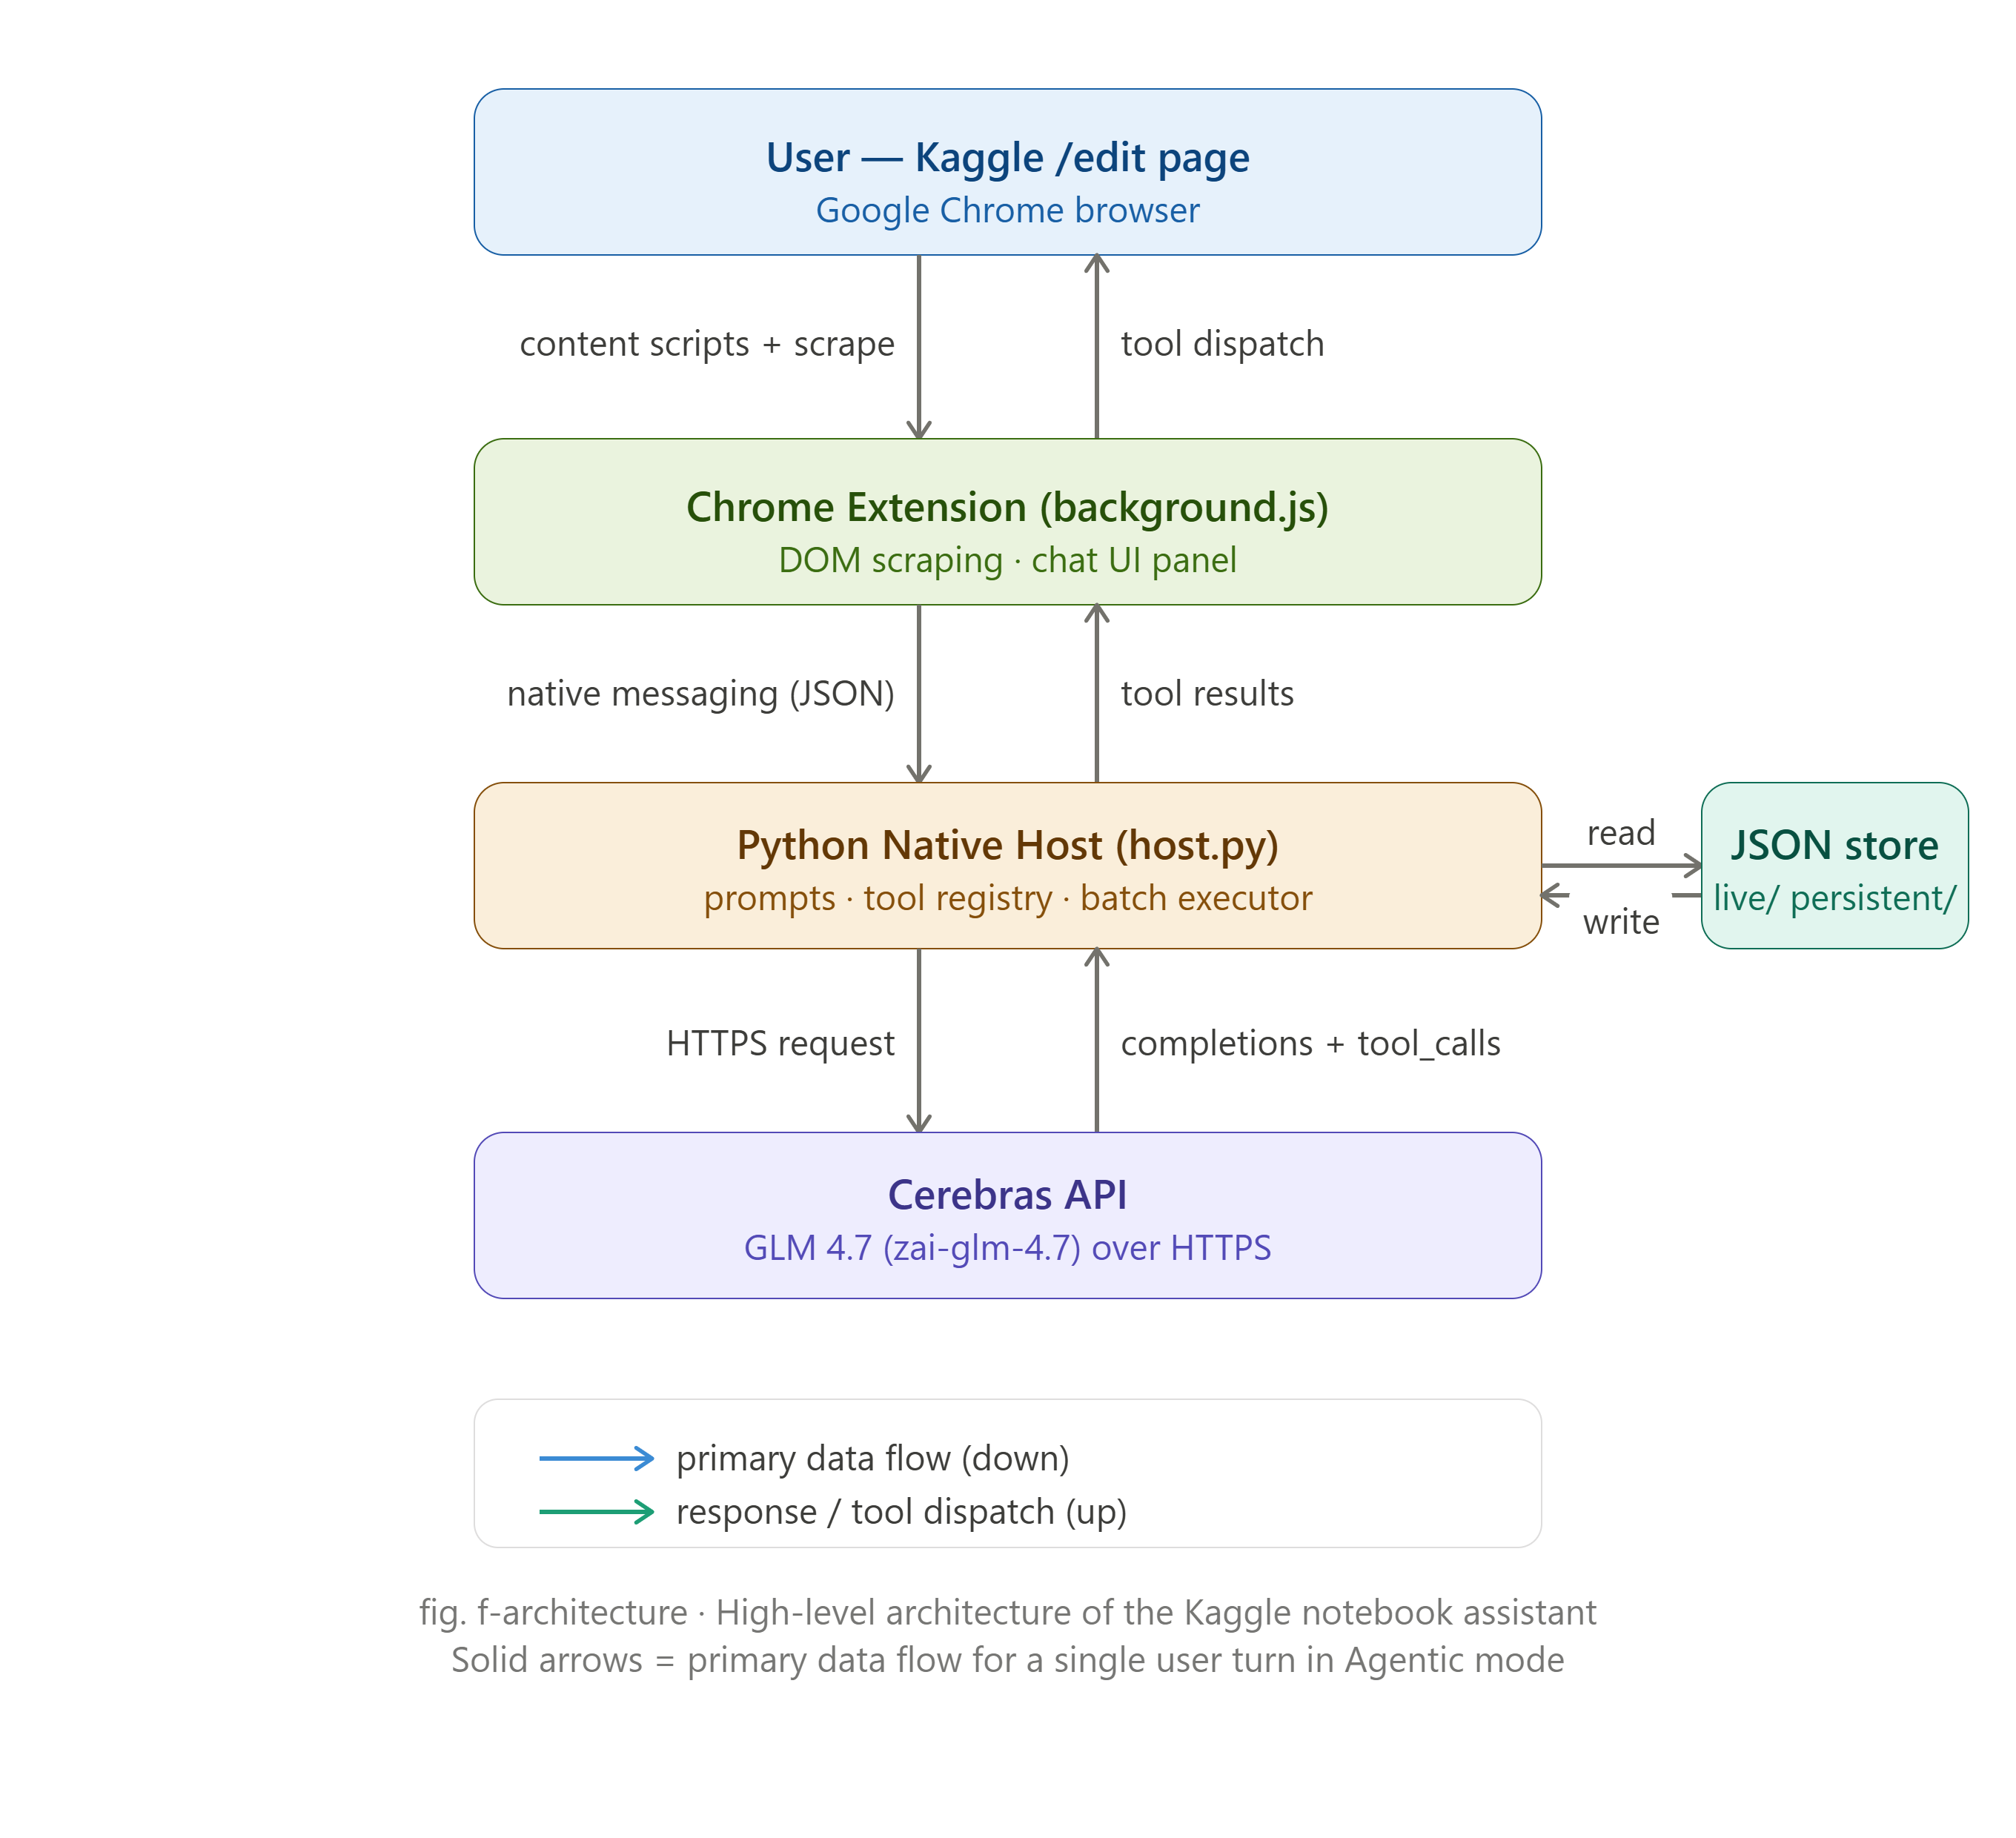
\includegraphics[width=0.95\textwidth]{f_architecture_system.png}
\caption{High-level architecture of the Kaggle notebook assistant. Solid arrows indicate primary data flow for a single user turn in Agentic mode.}
\label{f-architecture}
\end{figure}

Table~\ref{tab:components} summarises each layer's responsibility and primary artefacts.

\begin{table}[!ht]
\centering
\caption{Major system components and their roles.}
\label{tab:components}
\small
\begin{tabular}{|p{2.8cm}|p{4.2cm}|p{5.2cm}|}
\hline
\textbf{Component} & \textbf{Role} & \textbf{Key artefacts} \\ \hline
Chrome extension & \ac{DOM} scrape, chat interface, execute cell tools & \texttt{manifest.json}, \texttt{background.js}, content scripts \\ \hline
Native messaging bridge & Framed JSON over stdio between extension and host & Chrome native host manifest, \texttt{connectNative} port \\ \hline
Python host & \ac{LLM} orchestration, snapshots, tool dispatch, session keys & \texttt{host.py}, \texttt{tool\_registry.py}, \texttt{agentic\_batch\_executor.py} \\ \hline
Cerebras / GLM~4.7 & Remote inference with native \texttt{tool\_calls} & \texttt{cerebras\_client.py}, \texttt{llm\_provider.py} \\ \hline
Notebook JSON stores & Canonical cell lists for prompts and local tools & \texttt{live/}, \texttt{persistent/} under \texttt{data/notebooks/} \\ \hline
\end{tabular}
\end{table}

Three interaction modes govern host behaviour on each user message. \textbf{Ask} mode supplies conversational answers grounded in the current notebook snapshot without mutating cells. \textbf{Code} mode emphasises code-oriented assistance with the same grounding. \textbf{Agentic} mode enables the registered browser and local tools under a mandatory two-phase contract: round~0 is query-only (\texttt{notebook\_list\_cells}, \texttt{notebook\_get\_cell}); round~1 performs writes and runs (\texttt{insert\_cell}, \texttt{edit\_cell\_by\_index}, \texttt{delete\_by\_index}, \texttt{run\_cell}). Agentic mode is gated by both a host environment flag (\texttt{LLM\_AGENTIC\_ENABLED}) and the user's mode selection in the extension interface.

\section{Chrome Extension}
\label{sec:chrome-extension}

The extension targets Manifest~V3 and declares permissions for \texttt{tabs}, \texttt{nativeMessaging}, \texttt{scripting}, and \texttt{webNavigation}, with host permissions for \texttt{kaggle.com} and related Jupyter-proxy domains used by Kaggle's in-browser kernel. A service worker (\texttt{background.js}) maintains the native messaging port, coordinates tab-scoped scrape schedules, and routes host-issued commands to the correct frame and \texttt{tab\_id}. Figure~\ref{f-chrome-extension} shows the extension architecture and component structure.

\begin{figure}[!ht]
\centering
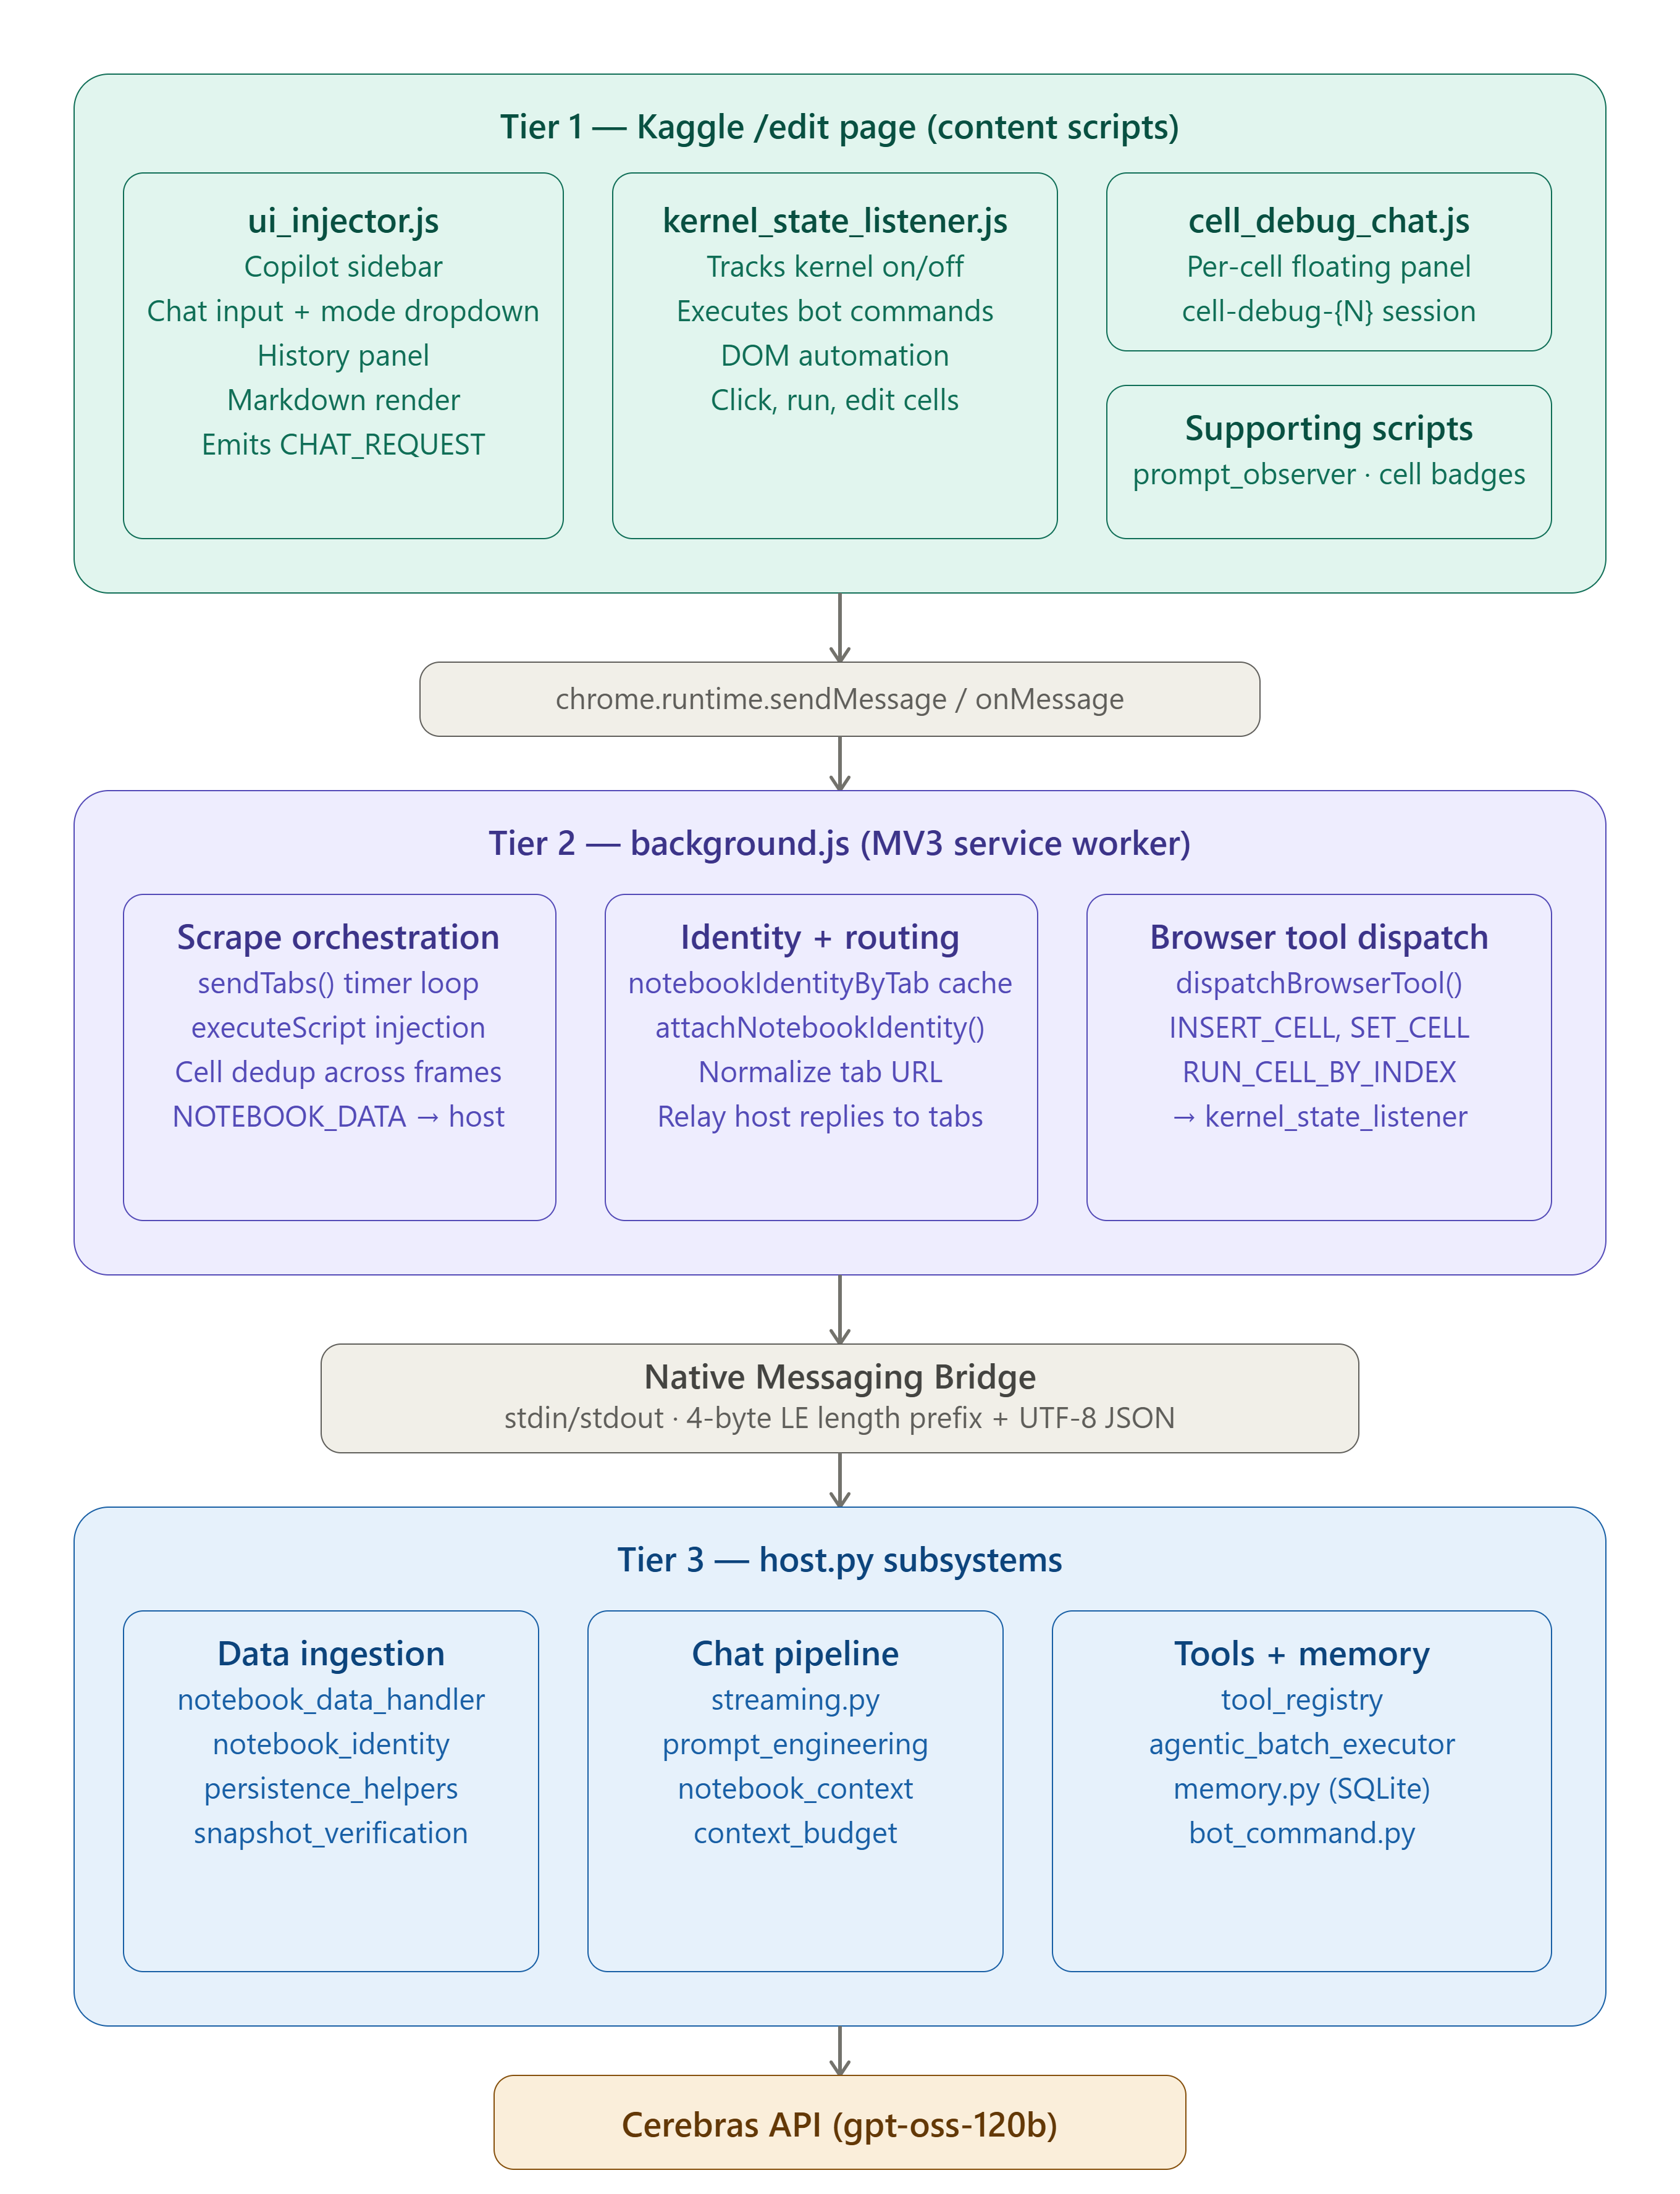
\includegraphics[width=0.95\textwidth]{chrome_extension_architecture_structure.png}
\caption{Chrome extension architecture and component structure.}
\label{f-chrome-extension}
\end{figure}

Content scripts run at \texttt{document\_start} on Kaggle notebook pages. They include utilities for cell indexing, kernel state observation, optional debug chat, and interface injection. Because Kaggle embeds notebook cells inside nested frames and shadow \ac{DOM} trees, scraping cannot assume a flat document: the function \texttt{scrapeNotebook()} walks the document, descends into open shadow roots and accessible iframes, and collects elements matching Jupyter-style selectors (\texttt{.jp-Cell}, \texttt{.code\_cell}, \texttt{.markdown\_cell}, and related markers).

For each collected cell, the scraper extracts:
\begin{itemize}
  \item positional index (application-visible, one-based where required for tool alignment);
  \item cell type (code versus markdown);
  \item source text from input areas;
  \item optional output text from output wrappers; and
  \item execution metadata where present in the \ac{DOM} (prompt numbers, button titles signalling queued, running, or executed state).
\end{itemize}

Scrape events are debounced and deduplicated to limit load on both the editor and the host. Figure~\ref{f-scrape-pipeline} illustrates the DOM scrape pipeline from editor cells to host ingestion.

\begin{figure}[!ht]
\centering
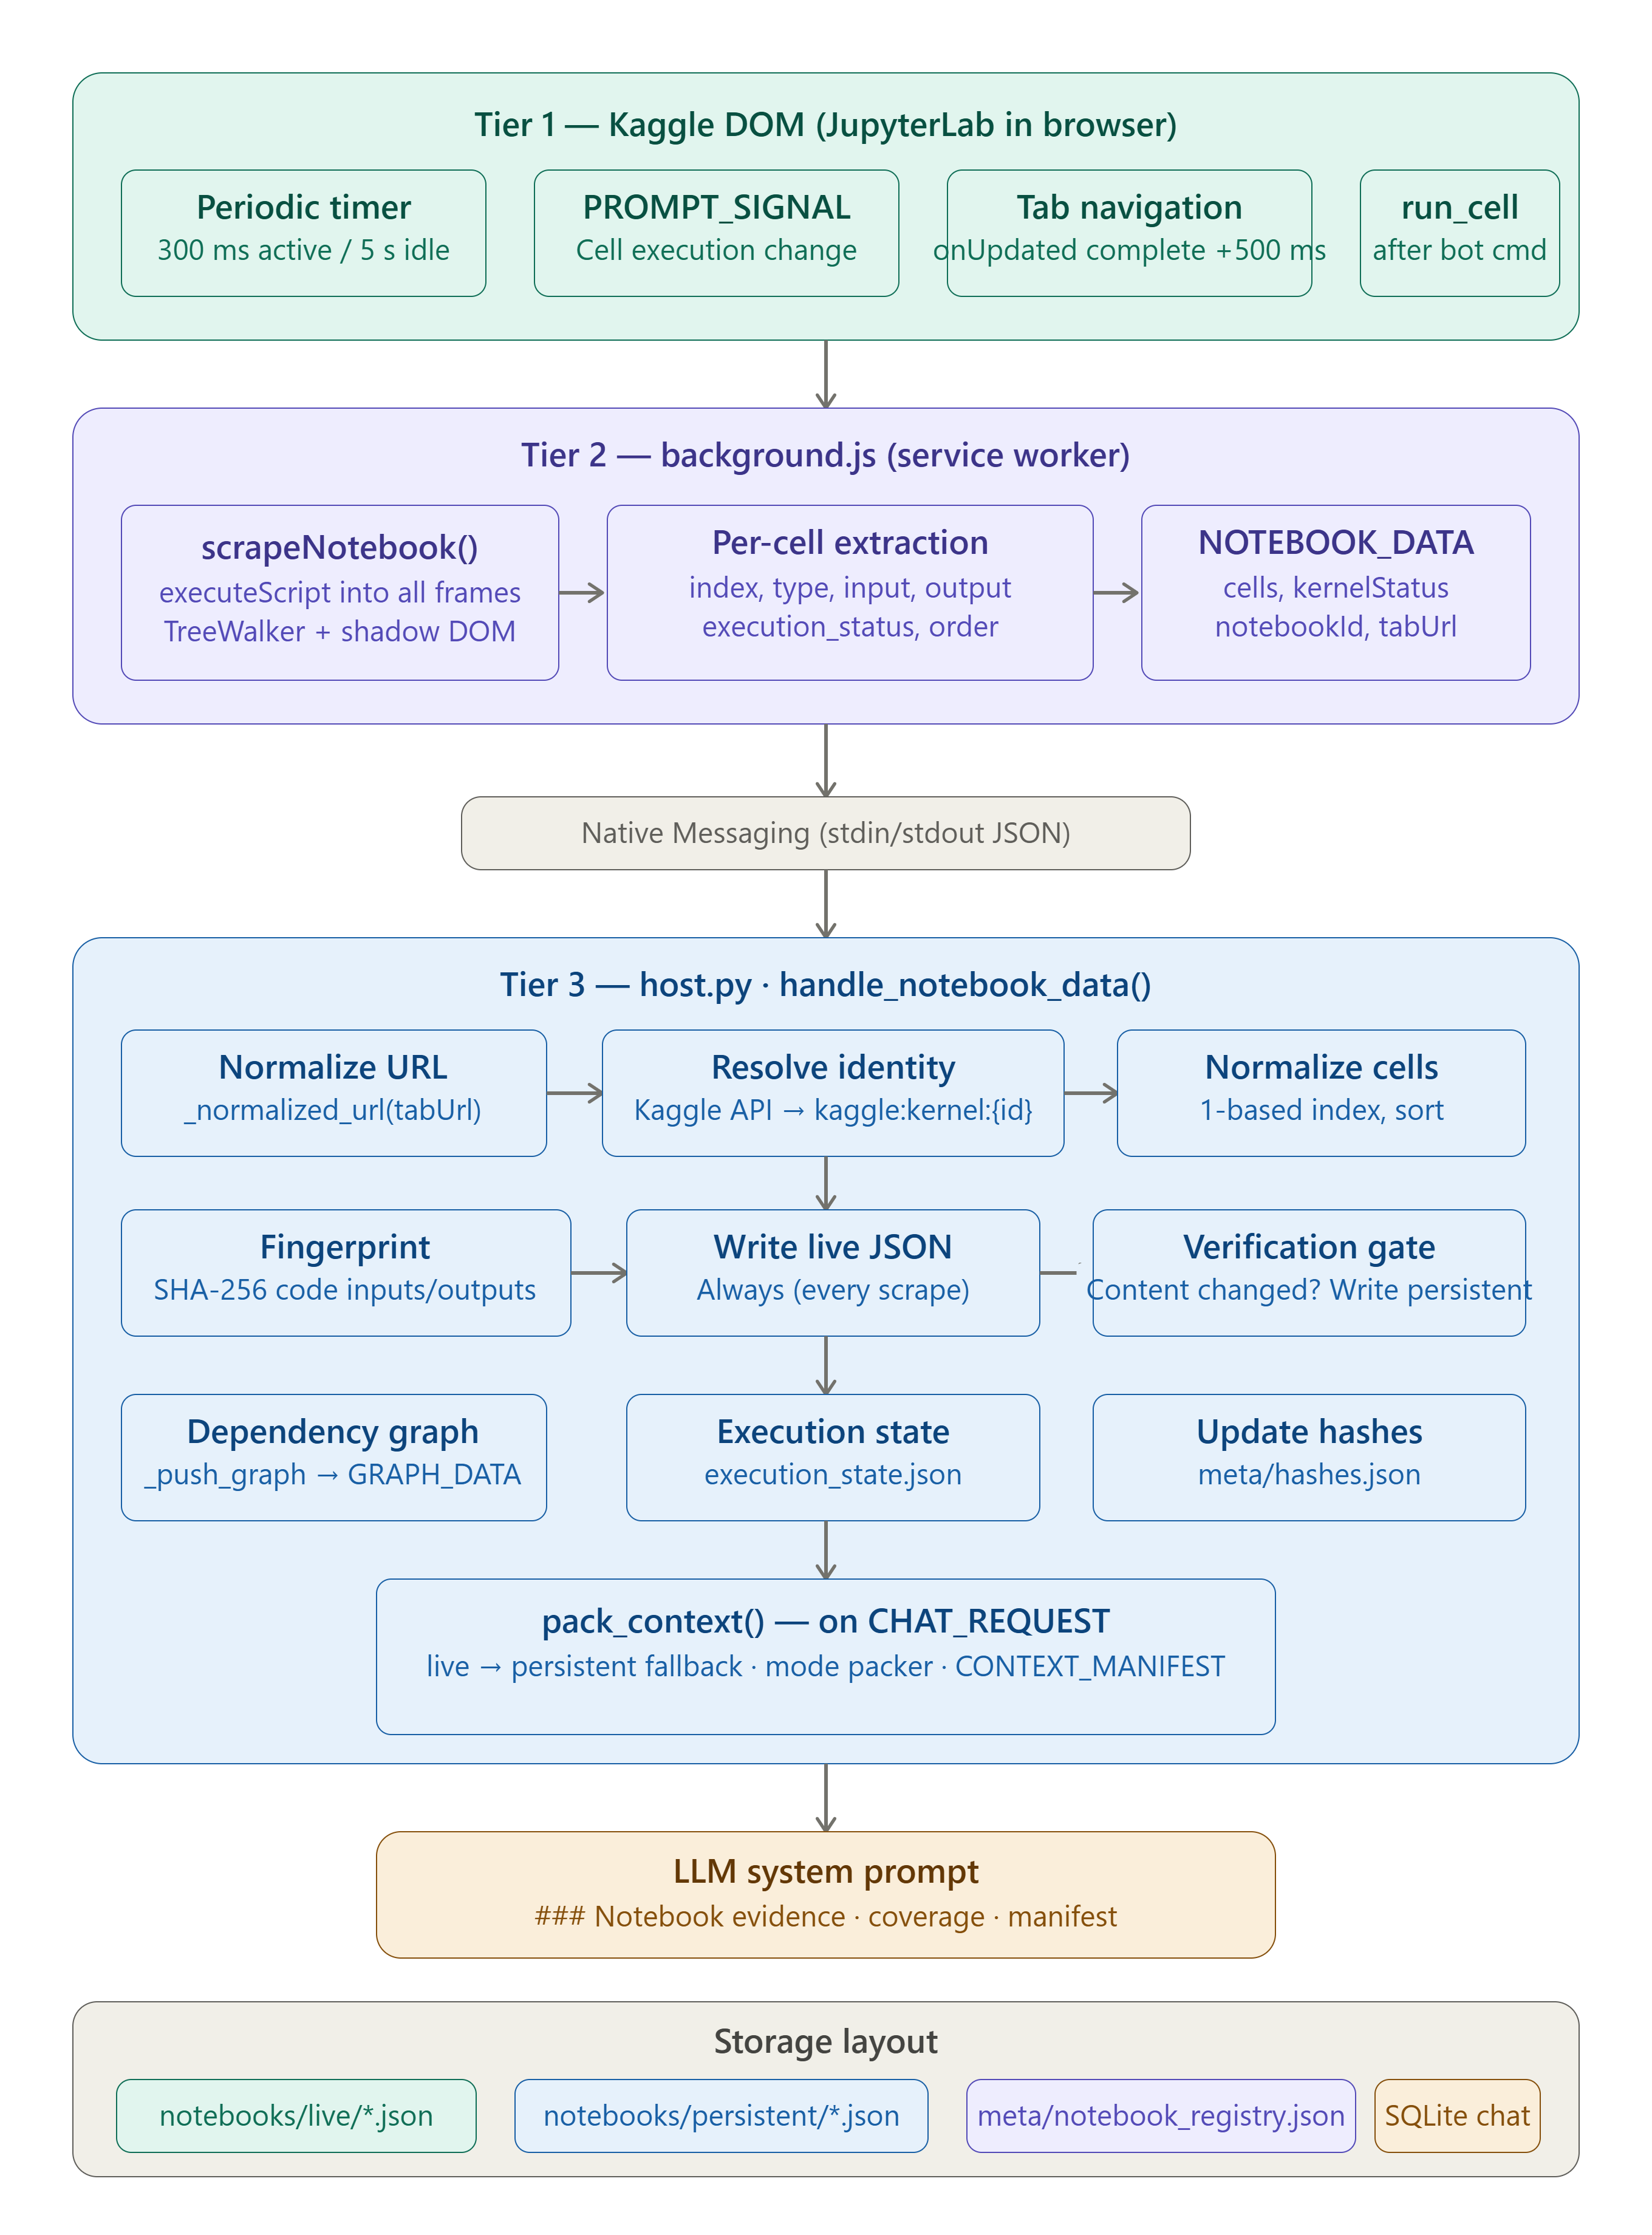
\includegraphics[width=0.95\textwidth]{notebook_scrape_pipeline_diagram.png}
\caption{Notebook DOM scrape pipeline from Kaggle editor to host ingestion.}
\label{f-scrape-pipeline}
\end{figure}

When a scrape completes, the extension forwards a structured payload---notebook URL, optional Kaggle kernel identifier, \texttt{tab\_id}, and the serialised cell list---to the host via native messaging. The extension also executes inverse operations when the host dispatches tool commands: inserting cells, editing source by index, deleting by index, running cells, and selecting or clicking cells to focus the editor. Each dispatch is correlated with the originating \texttt{tab\_id} so that multi-tab sessions do not cross-contaminate.

\section{Native Messaging Bridge}
\label{sec:native-messaging}

Chrome native messaging provides a length-prefixed JSON channel over standard input and output between the extension and the Python host process. The extension connects through \texttt{chrome.runtime.connectNative} to obtain a persistent port; messages are serialised as JSON objects with a \texttt{type} field that discriminates chat requests, notebook data uploads, tool commands, and results. Figure~\ref{f-native-messaging} summarises the bridge message flows.

\begin{figure}[!ht]
\centering
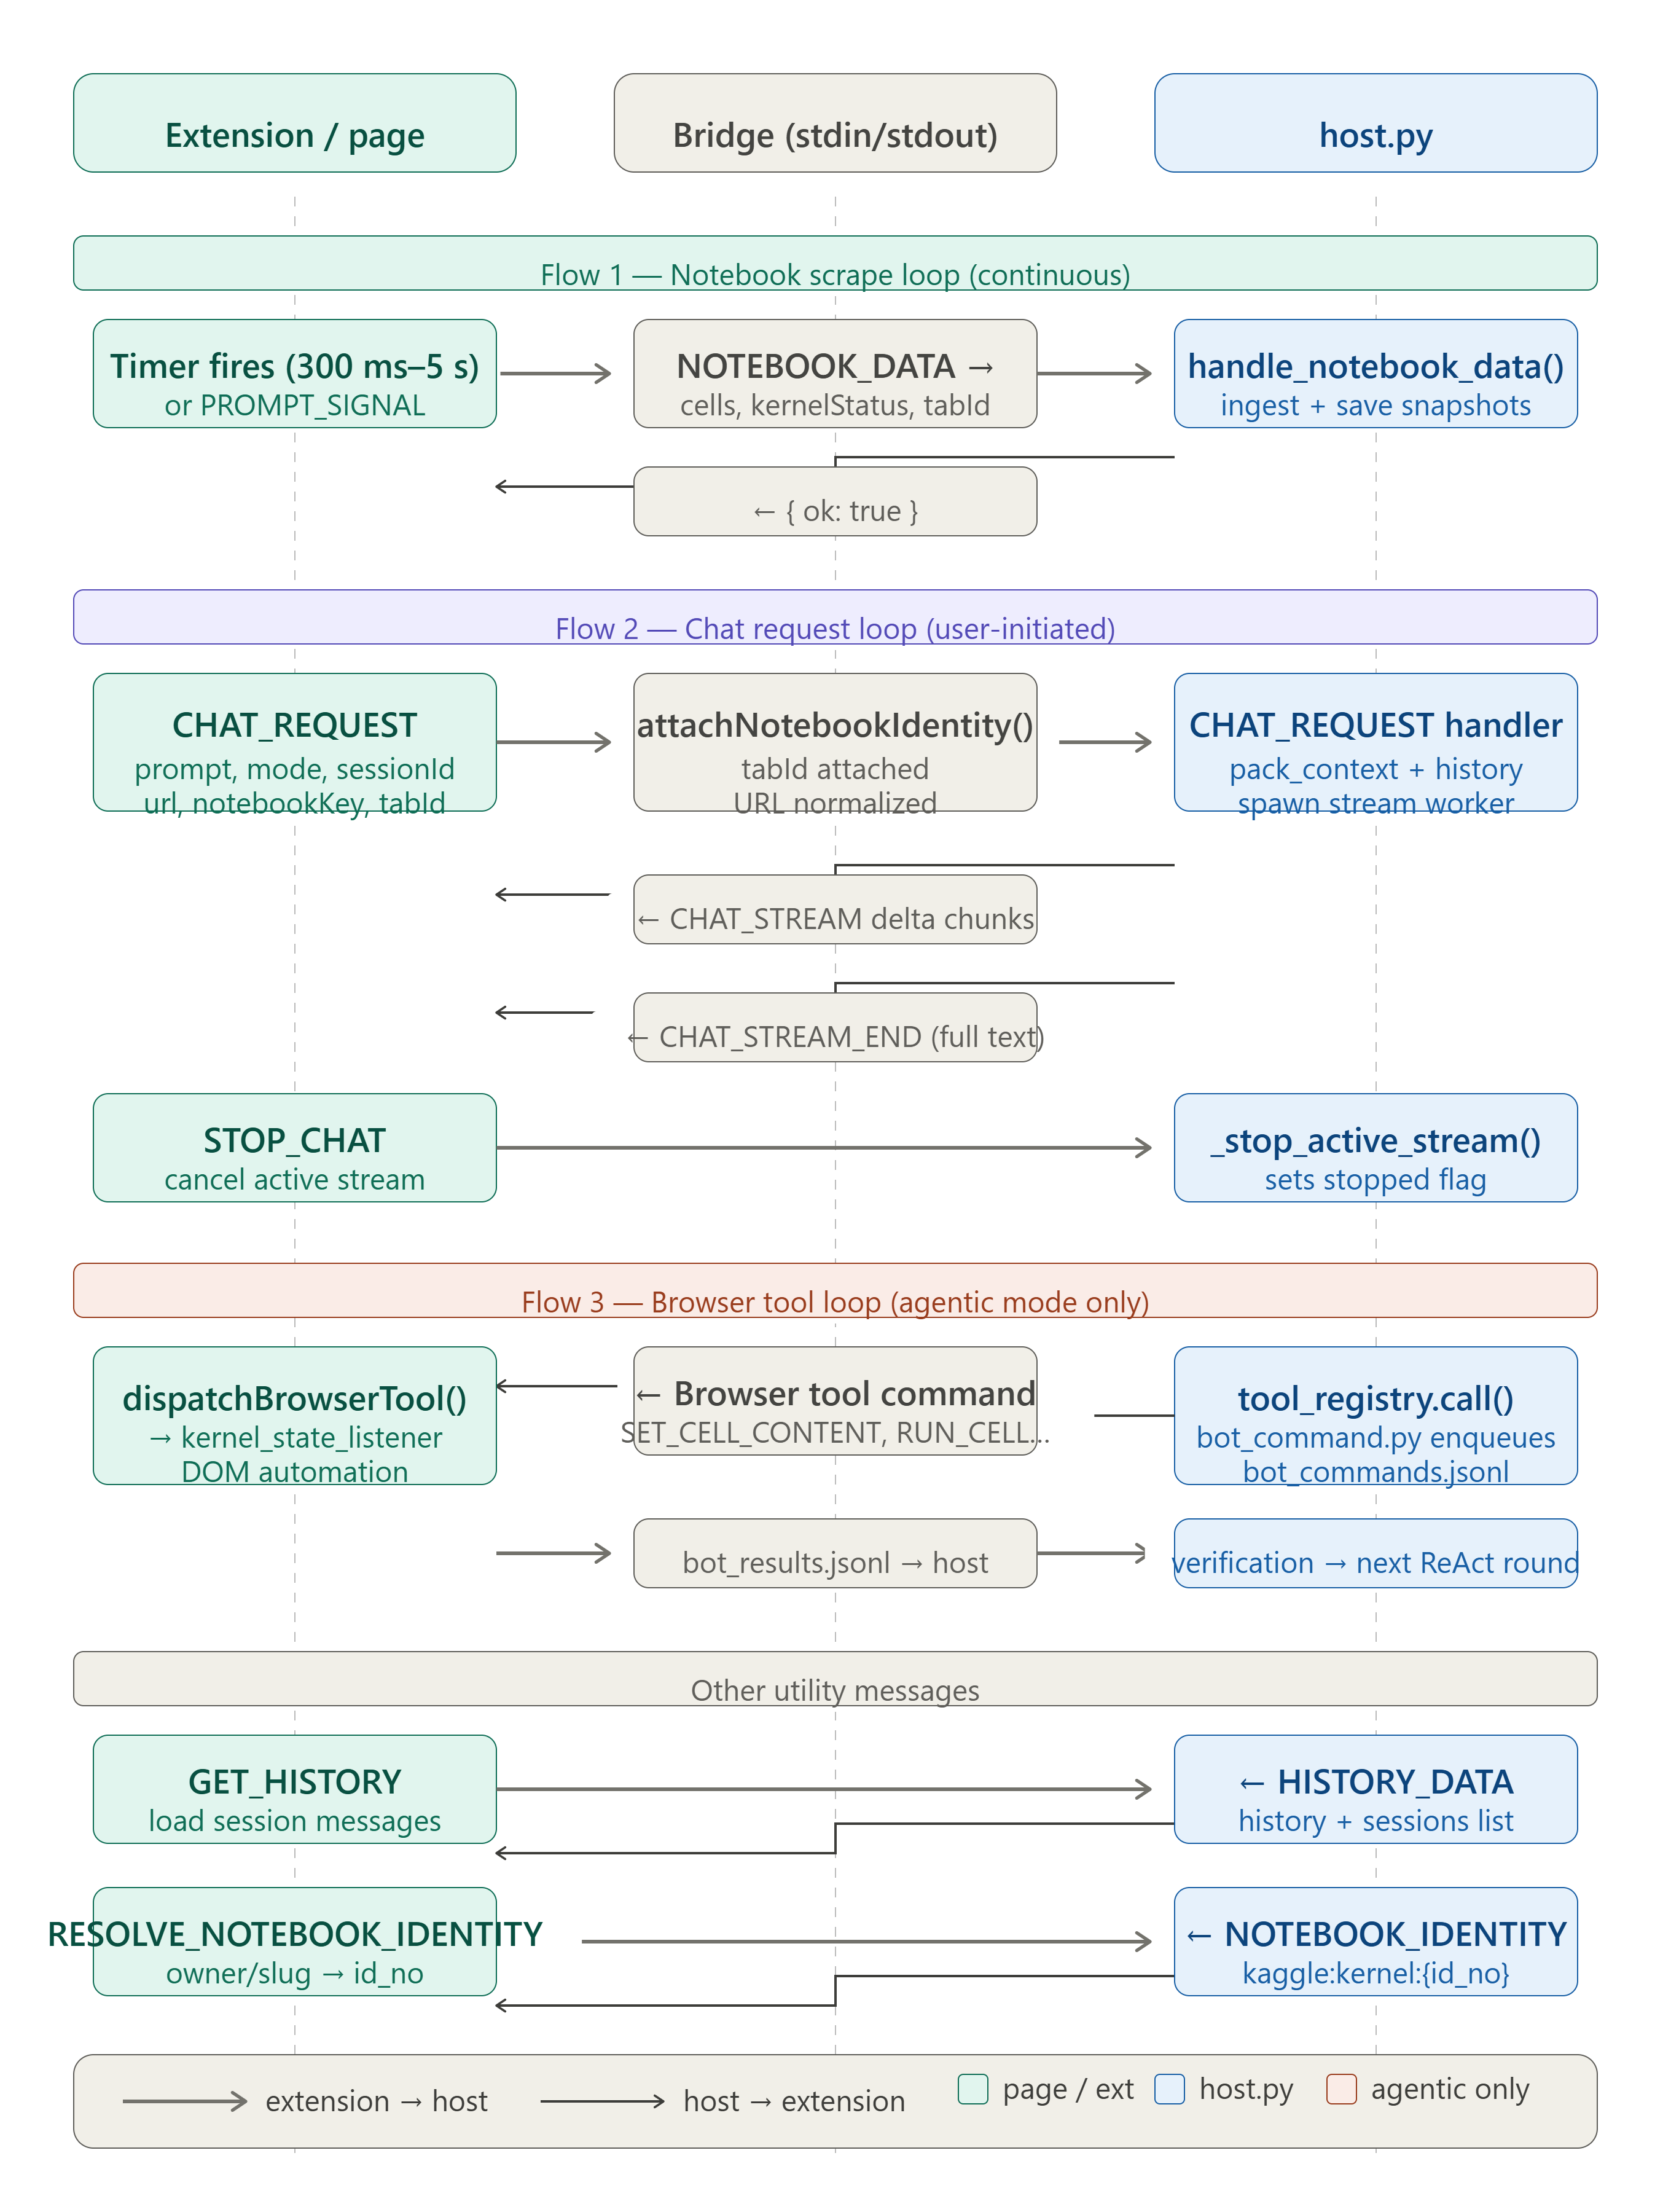
\includegraphics[width=0.95\textwidth]{native_messaging_bridge_flows.png}
\caption{Native messaging bridge message flows between extension and Python host.}
\label{f-native-messaging}
\end{figure}

The bridge enforces a strict process boundary. The extension never holds \ac{API} keys; the host never directly manipulates the \ac{DOM}. Tool arguments that omit session metadata are coerced on the host before dispatch: canonical notebook URL and \texttt{tab\_id} from the active chat turn are injected into each browser tool payload, satisfying Objective~3 in Section~\ref{sec:objectives}. Result messages use mirrored type names (for example, \texttt{INSERT\_CODE\_CELL\_RESULT} or error variants) so the host's stdin reader can pair completions with pending tool calls.

This design trades remote deployability for local installation overhead: the user must register the native host manifest with Chrome. In return, the assistant gains stable, full-duplex communication without exposing a network listener on the public internet; the host binds an optional local HTTP endpoint (\texttt{127.0.0.1:8080}) for development dashboards only.

\section{Python Native Host}
\label{sec:python-host}

The host entry point is \texttt{host.py} under \texttt{testing/host/}. On startup it loads \texttt{config.py} and initialises directories under \texttt{testing/host/data/}. The dispatcher starts the native messaging I/O loop. Messages route to \texttt{notebook\_data\_handler.py} for ingestion and to \texttt{streaming.py} for chat. Tool execution uses \texttt{tool\_registry.py}; the batch executor module handles batched dispatch.

\subsection{Prompt assembly and chat modes}
\label{sec:prompt-assembly}

Prompt templates reside under \texttt{testing/host/prompts/}, with mode-specific files for Ask, Code, and Agentic behaviour. The module \texttt{prompt\_engineering.py} composes the message list sent to the \ac{API}: a base notebook-assistant system prompt, Jupyter structure guidance, mode instructions, a packed notebook context slice, and recent chat history subject to token budgets ({\ttfamily\seqsplit{MAX\_INPUT\_TOKENS}} and {\ttfamily\seqsplit{MAX\_NOTEBOOK\_CONTEXT\_CHARS}}). Context packing can operate in \texttt{full} or \texttt{intent} mode; the default favours complete cell lists when token limits allow, supporting faithful positional references in tool arguments. Figure~\ref{f-context-packing} depicts the context-packing and notebook-intelligence pipeline.

\begin{figure}[!ht]
\centering
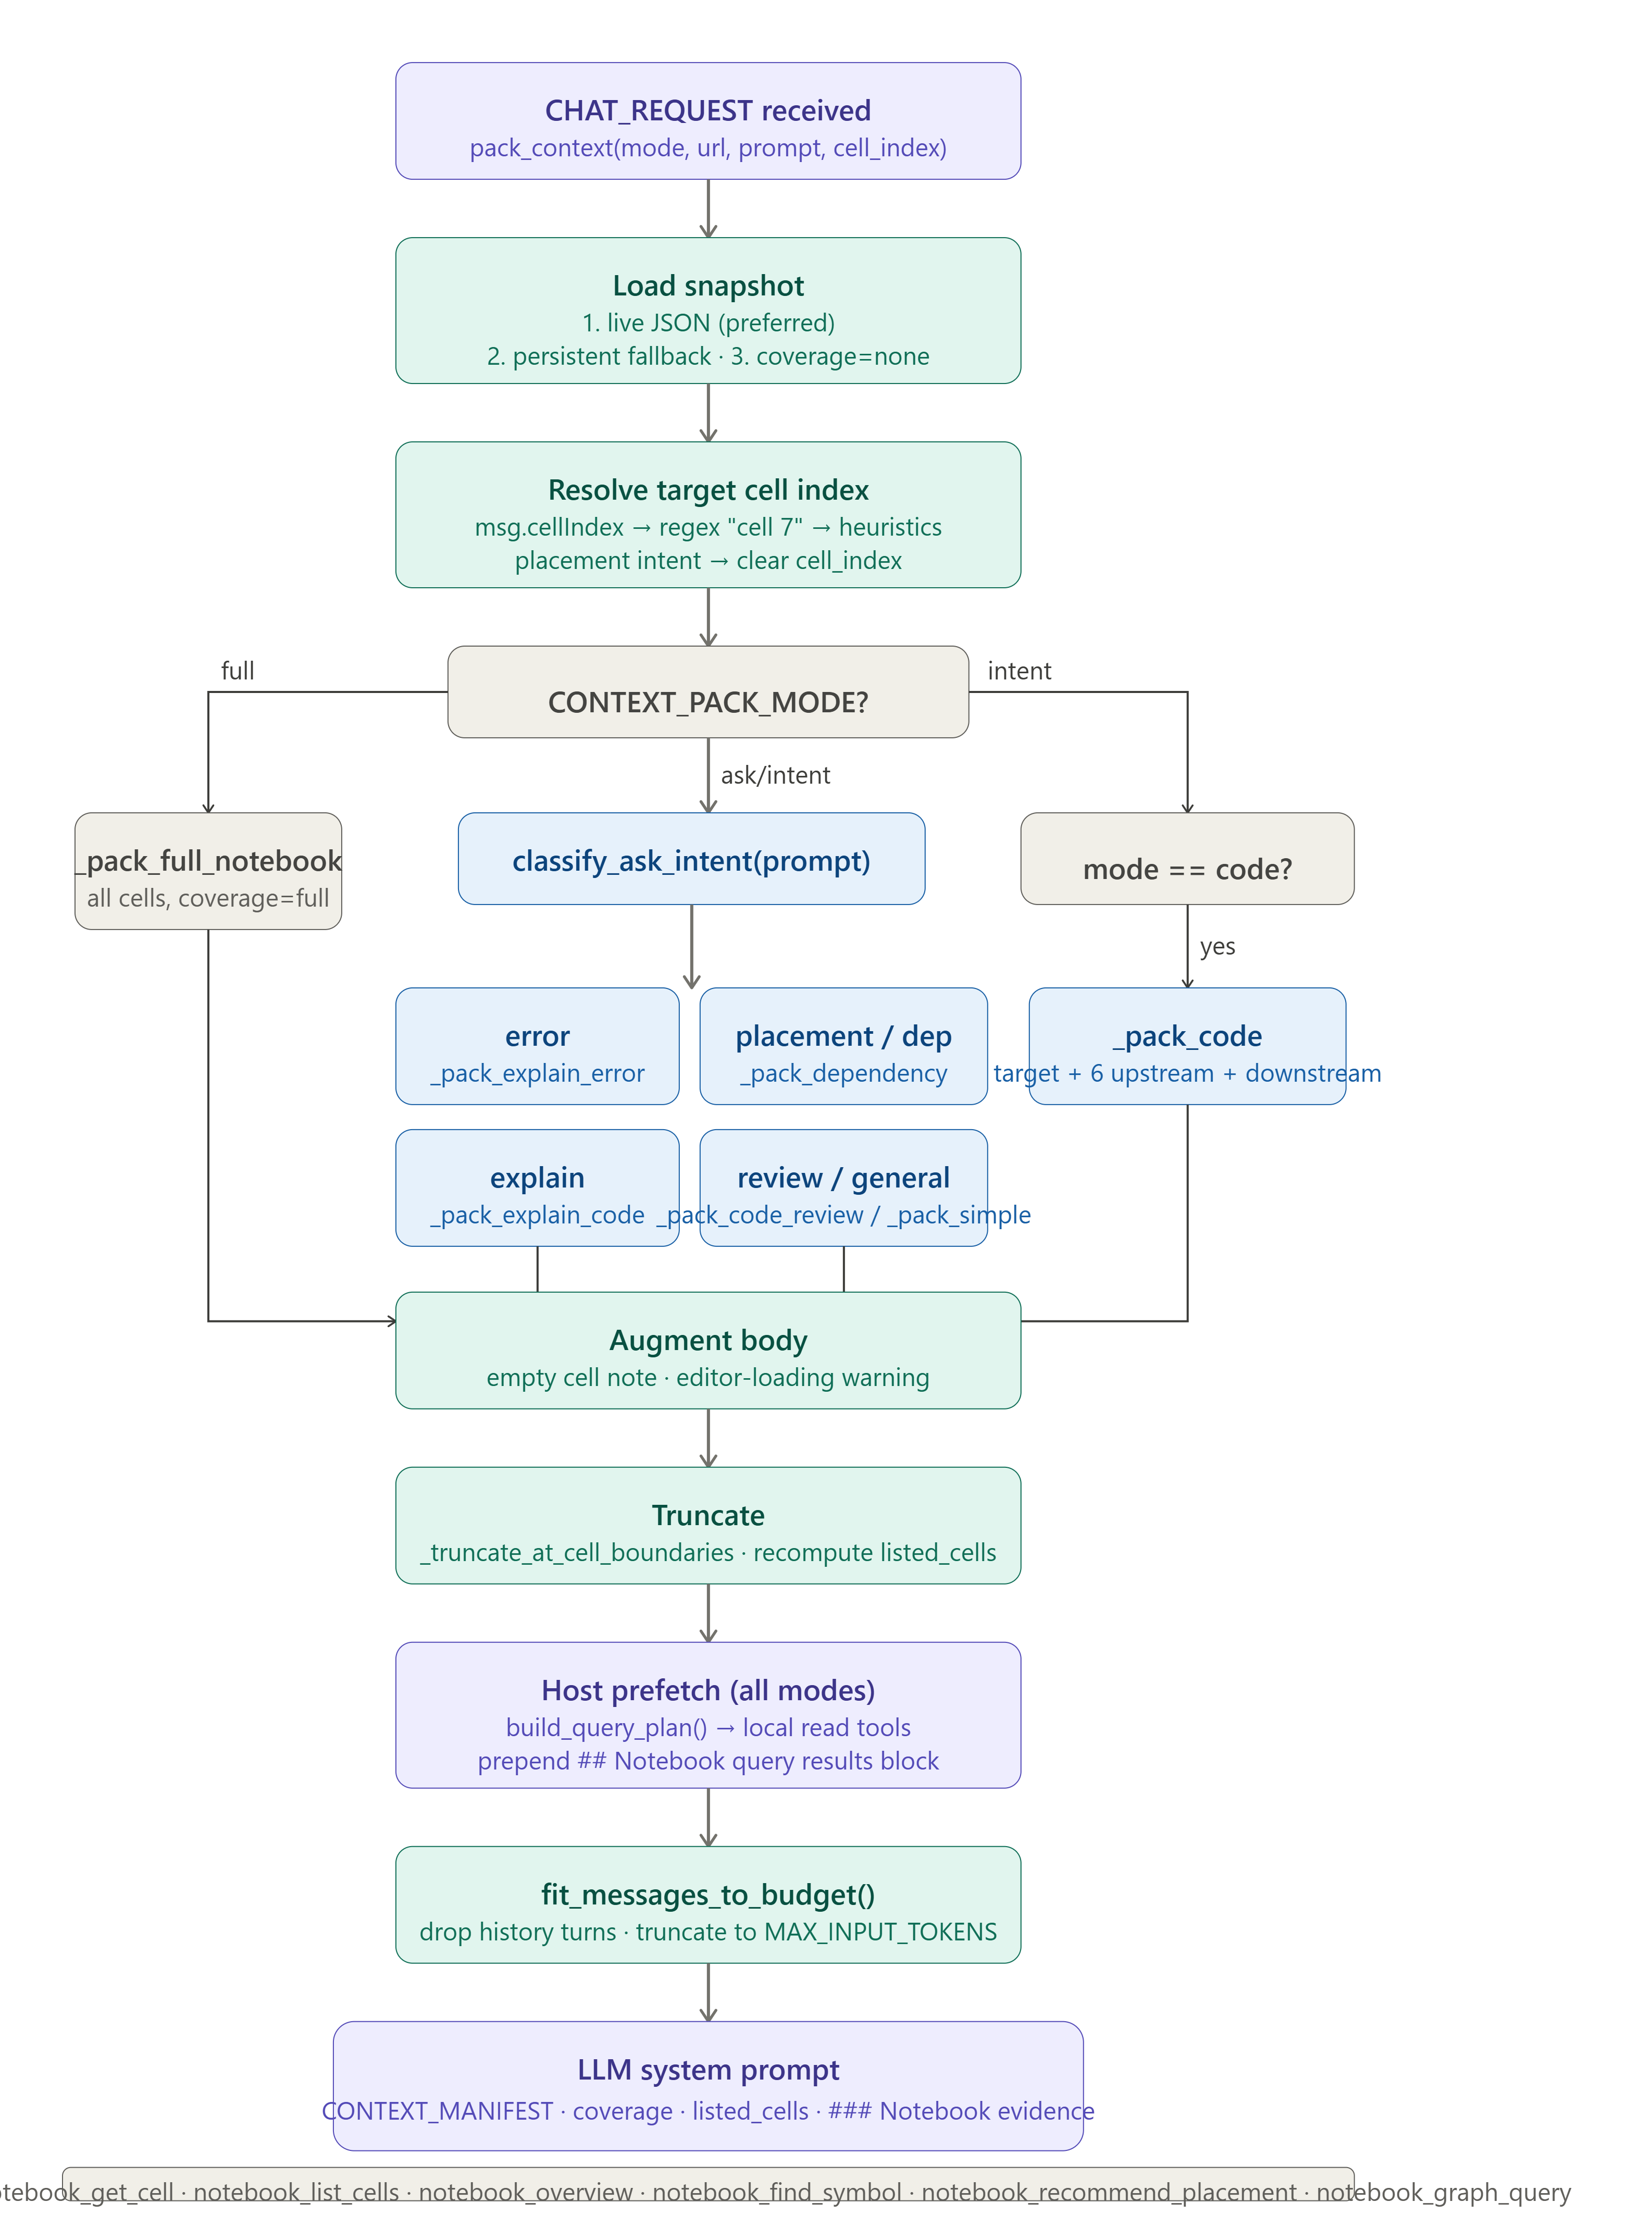
\includegraphics[width=0.95\textwidth]{context_packing_notebook_intelligence.png}
\caption{Context packing and notebook intelligence pipeline on the host.}
\label{f-context-packing}
\end{figure}

Chat history is keyed by a stable notebook identity resolved from the Kaggle kernel id when available ({\ttfamily\seqsplit{kaggle:kernel:<id>}}). A normalised URL fallback uses \texttt{notebook\_identity.py}. This key aligns snapshot filenames, SQLite session storage, and tool \texttt{url} arguments.

\subsection{Tool registry and agentic execution contract}
\label{sec:tool-registry}

Tools are registered in \texttt{tool\_registry.py} with JSON-schema argument validation. They fall into two classes:
\begin{itemize}
  \item \textbf{Local read tools} execute entirely on the host against persisted JSON snapshots. Examples include \texttt{notebook\_list\_cells}. Cell bodies use \texttt{notebook\_get\_cell}. Status queries use \texttt{notebook\_snapshot\_status}.
  \item \textbf{Browser tools} are forwarded to the extension for \ac{DOM} operations. Examples include \texttt{insert\_cell}, \texttt{edit\_cell\_by\_index}, \texttt{delete\_by\_index}, and \texttt{run\_cell}.
\end{itemize}

Agentic execution is governed by configuration flags in \texttt{config.py}:
\begin{itemize}
  \item {\ttfamily\seqsplit{AGENTIC\_MANDATORY\_TWO\_PHASE}} (default on): round~0 strips write tools; round~1 strips redundant list/query tools.
  \item {\ttfamily\seqsplit{AGENTIC\_MAX\_TOOL\_ROUNDS}} (default 2): hard cap on \ac{LLM} \ac{API} calls per user message.
  \item {\ttfamily\seqsplit{AGENTIC\_FIRE\_AND\_FORGET}} (default on): the host dispatches an ordered tool batch without waiting for per-cell snapshot reconciliation before the model's implement round completes.
\end{itemize}

The batch executor (\texttt{agentic\_batch\_executor.py}) builds the tool queue. Rules from \texttt{strict\_execution\_engine.py} sort bulk deletes and inserts in \emph{descending} index order, then \texttt{run\_cell} actions. Dispatches are logged through \texttt{tool\_call\_terminal.py}.

Scrape-based observers include \texttt{cell\_execution\_observer.py}. Layout tracking uses \texttt{cell\_structure\_observer.py}. They supply scrape-based feedback without closed-loop replanning.

\section{LLM Integration: GLM~4.7 via Cerebras}
\label{sec:llm-integration}

Remote inference uses the Cerebras \ac{API} with model identifier \texttt{zai-glm-4.7} (GLM~4.7), configured through \texttt{CEREBRAS\_MODEL} in the environment. The client module \texttt{cerebras\_client.py} submits chat completions with tool definitions generated from the registry and prompt autogen files under \texttt{prompts/tool\_calling/}. GLM~4.7 supports \emph{native parallel} \texttt{tool\_calls} in a single completion when the model can plan an entire implement batch at once; the provider module \texttt{llm\_provider.py} records this capability and applies Cerebras free-tier rate limits (requests and tokens per minute).

Temperature and top-$p$ are set conservatively (\texttt{LLM\_TEMPERATURE} default 0.5) to favour deterministic tool selection over creative variation. When Agentic mode is active and the server allows it, tool schemas are attached to the completion request; the host parses returned \texttt{tool\_calls}, validates arguments, applies phase guards, and either executes local tools immediately or enqueues browser tools for the extension. Streaming responses (\texttt{streaming.py}) support incremental user-interface updates in Ask and Code modes; Agentic batches may still stream textual narration while tools are queued.

\pagebreak[4]
The integration is intentionally single-provider for the FYP artefact: \texttt{LLM\_PROVIDER} normalises to \texttt{cerebras}, keeping evaluation comparable and configuration reproducible. \ac{API} keys reside only in the host environment (\texttt{CEREBRAS\_API\_KEY}), never in the extension package.

\section{Notebook JSON Persistence}
\label{sec:notebook-json}

Notebook state is materialised as JSON documents under \texttt{testing/host/data/notebooks/}, managed by \texttt{notebook\_storage.py} and \texttt{persistence\_helpers.py}. Each notebook is addressed by a \emph{storage key}: preferentially \texttt{kaggle:kernel:<numeric\_id>}, which maps to filenames such as \texttt{kaggle\_kernel\_112732919.json}; if no kernel id is known, a sanitised URL slug is used instead. Figure~\ref{f-notebook-persistence} shows data ingestion and persistence across live and persistent stores.

\begin{figure}[!ht]
\centering
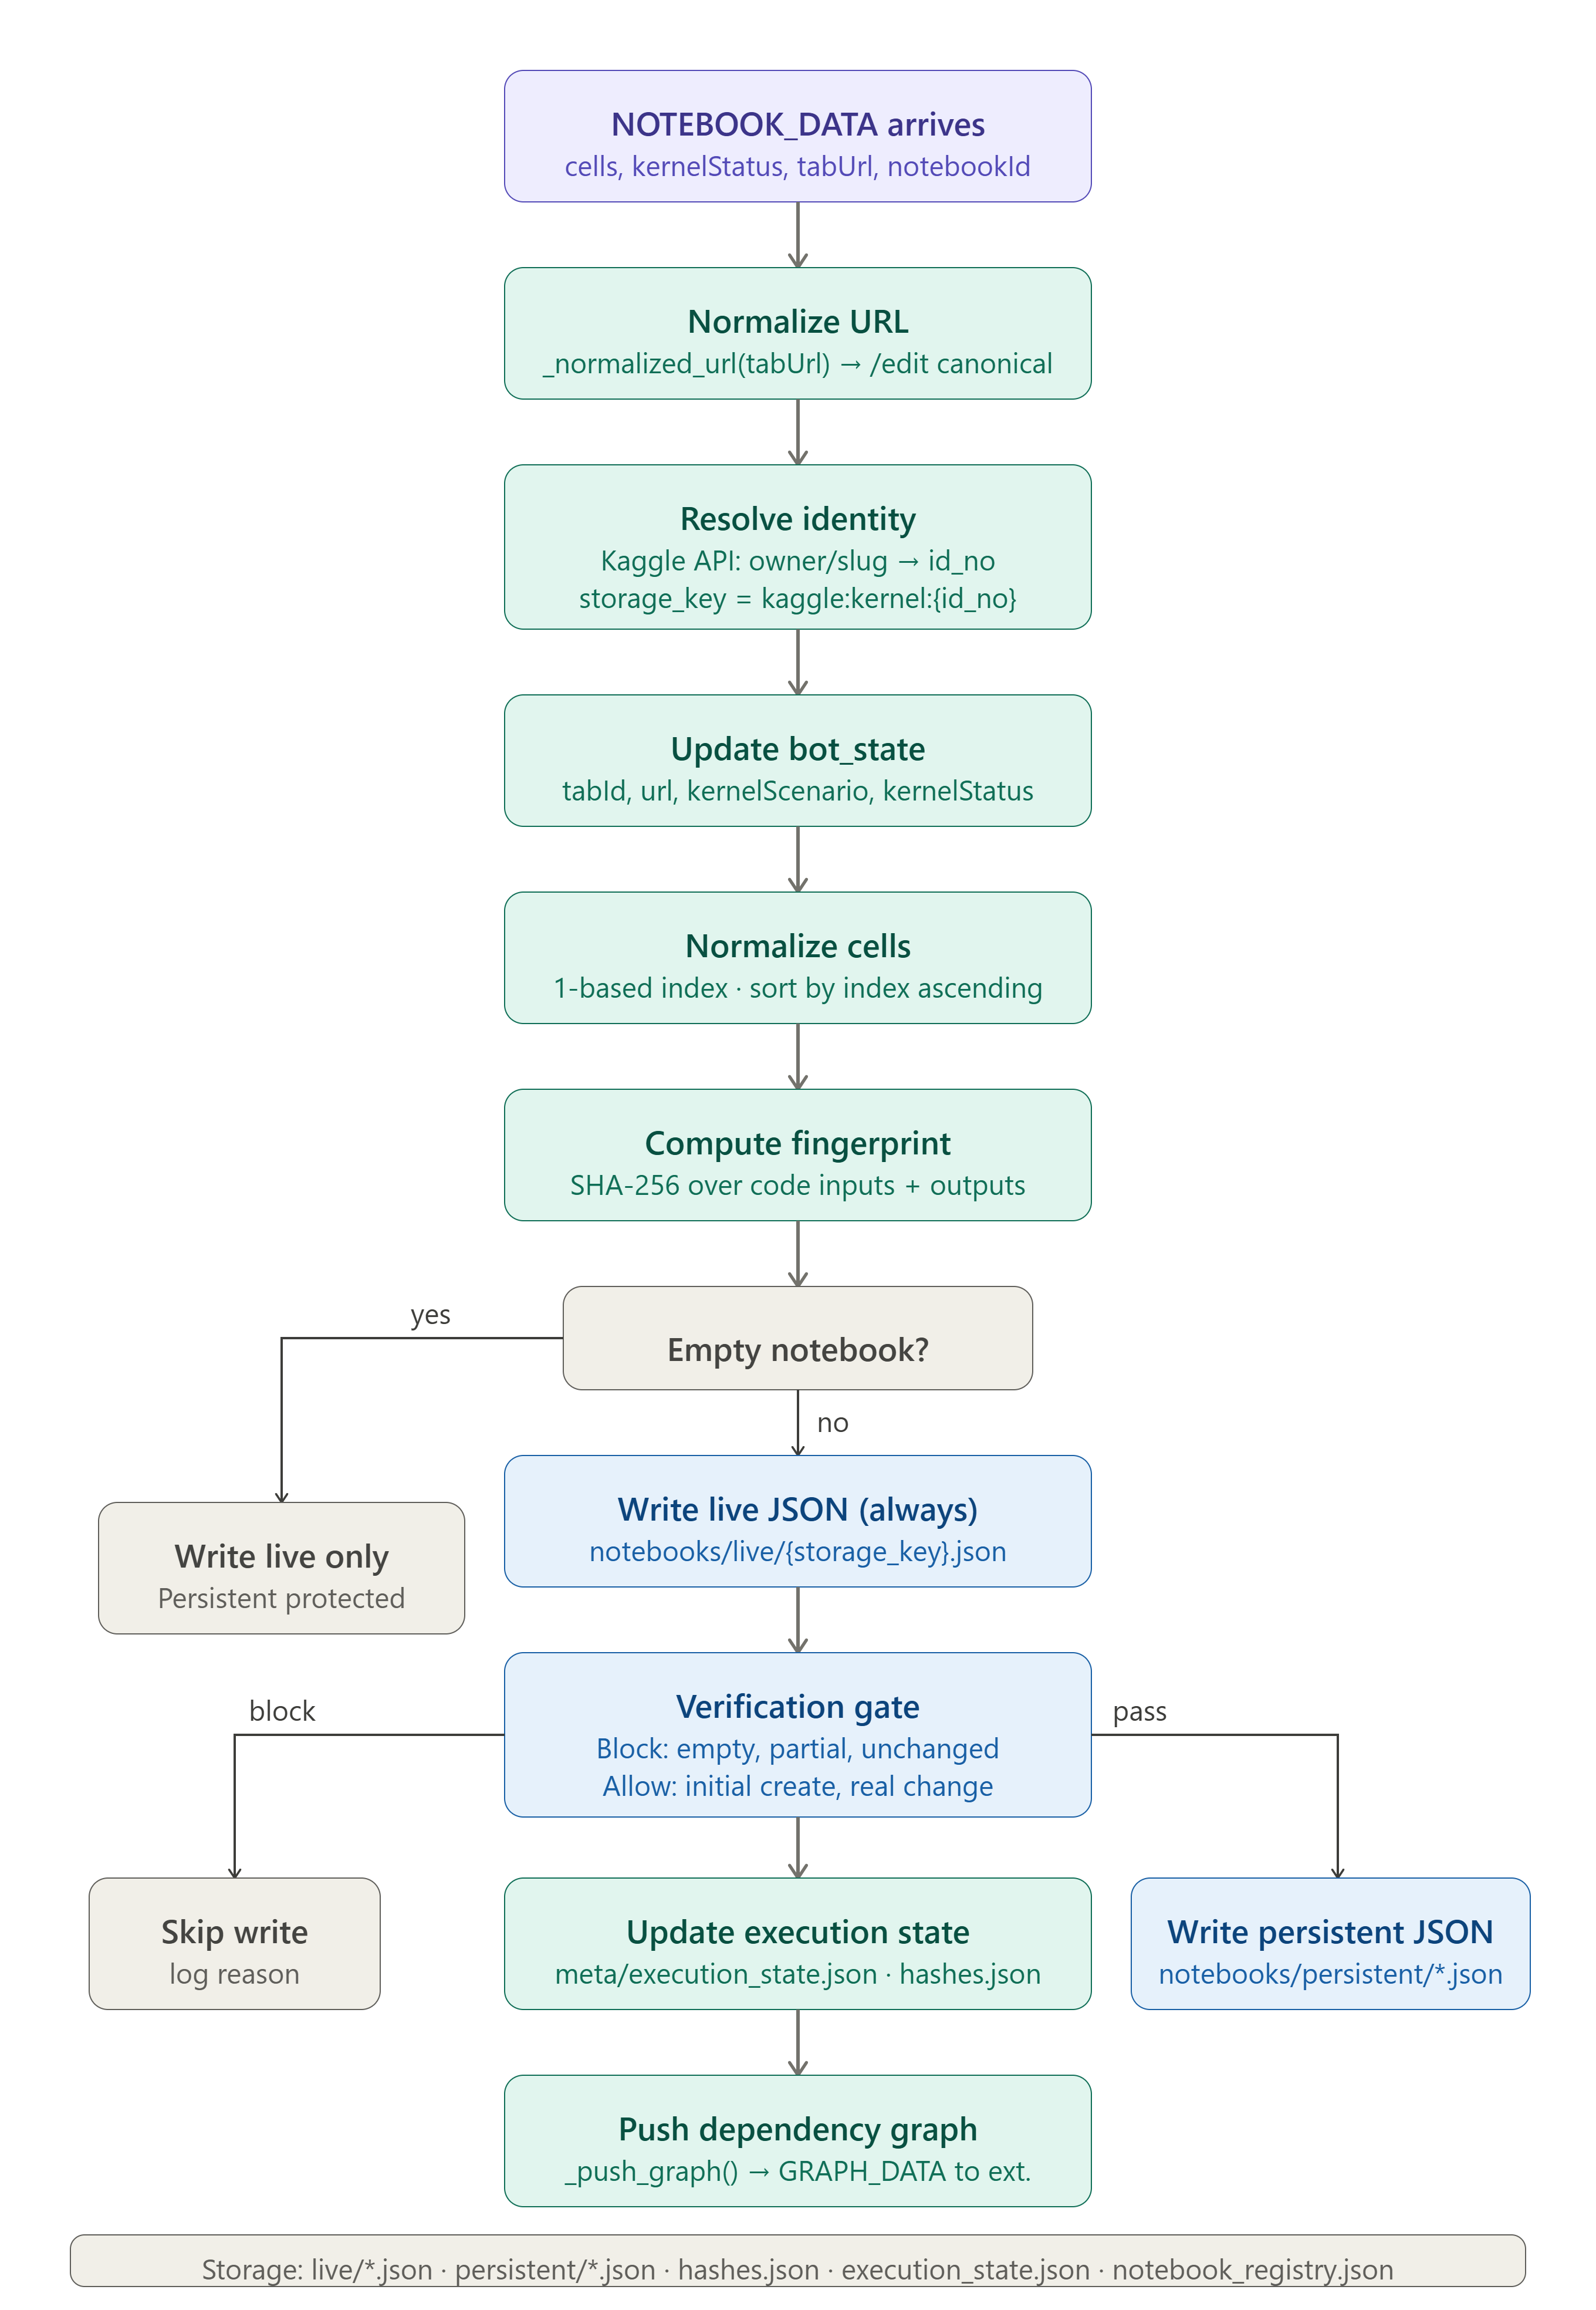
\includegraphics[width=0.95\textwidth]{notebook_data_ingestion_persistence.png}
\caption{Notebook data ingestion and persistence across live and persistent JSON stores.}
\label{f-notebook-persistence}
\end{figure}

Two parallel stores exist for every key:
\begin{itemize}
  \item \textbf{Live} (\texttt{live/}): updated on each successful scrape from the extension. Reflects the notebook as currently rendered, including cells the user has not yet saved to a long-term Kaggle revision.
  \item \textbf{Persistent} (\texttt{persistent/}): updated when scrapes pass verification checks and after successful browser tool mutations (via \texttt{sync\_persistence\_for\_action} in the tool registry). Serves as the durable baseline for prompts and local read tools when live data is temporarily unavailable.
\end{itemize}

Each JSON document follows a common schema: a top-level \texttt{cells} array with objects carrying index, type, source, optional outputs, and execution metadata fields stripped or retained according to \texttt{KERNEL\_EXECUTION\_METADATA\_ENABLED}. Hash and execution-state sidecars under \texttt{data/meta/} detect whether a new scrape materially changes structure or run status, reducing redundant writes and supporting monitor scripts.

This dual-store design implements the context-grounding strategy from Section~\ref{sec:lit-rag}: the \ac{LLM} is not given a static file export but a continuously refreshed, positional cell list aligned with the user's session. Live snapshots maximise freshness; persistent snapshots maximise availability across turns and brief navigation away from the editor. Together they enable the host to inject notebook context into every mode without manual copy-and-paste from the user.

\section{Evaluation Design}
\label{sec:evaluation}

Empirical evaluation assesses whether the three interaction modes---Ask, Code, and Agentic---behave according to their declared contracts when grounded in frozen Kaggle notebook snapshots. Experiments were executed with GLM~4.7 (\texttt{zai-glm-4.7}) via the Cerebras \ac{API}, using harness scripts under \texttt{testing/host/scripts/}. Each suite comprises four scenario tests aligned with mode-specific objectives identified in the literature on notebook assistants \parencite{mcnutt2023notebookassistants} and tool-augmented language models \parencite{qin2024toolllm,yao2023react}.

\subsection{Benchmark suites}

\textbf{Ask mode} measures explanation quality only: no code generation, no tool execution, and no notebook modification. Tests cover notebook workflow explanation, single-cell explanation, error diagnosis, and empty-cell handling. Metrics include topic coverage, evidence alignment, and a heuristic hallucination rate derived from snapshot ground truth.

\textbf{Code mode} measures code-generation quality in chat: runnable \texttt{python} blocks, placement guidance, and run-order instructions, without browser writes. Metrics include code-correctness (keyword alignment with notebook variables) and placement accuracy (cited cell indices relative to notebook flow).

\textbf{Agentic mode} measures \emph{LLM tool dispatch} under the mandatory two-call contract. Each user task consumes exactly two \ac{API} calls. In \emph{round~0}, the model may issue read-only notebook queries such as \texttt{notebook\_list\_cells} and \texttt{notebook\_get\_cell}. In \emph{round~1}, it emits the implement batch---including \texttt{insert\_cell}, \texttt{edit\_cell\_by\_index}, and \texttt{run\_cell}---which the host dispatches in fire-and-forget mode without a closed-loop ReAct replanning cycle \parencite{yao2023react,shinn2023reflexion}. Success is judged by dispatch fidelity of tool types, not by post-hoc execution verification (which the current artefact does not implement).

\subsection{Notebooks and harness}

Benchmarks used persistent JSON snapshots from public Kaggle kernels \parencite{quaranta2021kgtorrent}. Primary fixtures were Pakistan housing ({\ttfamily\seqsplit{kaggle\_kernel\_113620421.json}}) and testing-ol ({\ttfamily\seqsplit{kaggle\_kernel\_112732919.json}}). The harness replays chat requests through \texttt{streaming.py} with browser tools mocked at the extension boundary. Trace logs are written to {\ttfamily\seqsplit{agentic\_tool\_trace.jsonl}}.

\subsection{Limitations of the evaluation protocol}

Results characterise \emph{dispatch fidelity} and \emph{mode-contract compliance} under snapshot grounding. They do not constitute a live Kaggle \ac{DOM} study or a human expert rubric. Agentic scores therefore reflect planning and batching behaviour within the two-call cap rather than full autonomous notebook completion. A future release could add a ReAct-style observe--act loop \parencite{yao2023react} with per-cell feedback; that capability is explicitly out of scope for the present version.

\section{Interaction Mode Specifications}
\label{sec:mode-specs}

Each mode is enforced at three layers: the extension user-interface dropdown, host-side mode resolution in \texttt{streaming.py}, and prompt/tool-filter rules in \texttt{prompt\_engineering.py}. Table~\ref{tab:mode-contracts} states the behavioural contract evaluated in Chapter~\ref{c-results}.

\begin{table}[!ht]
\centering
\caption{Interaction mode contracts.}
\label{tab:mode-contracts}
\footnotesize
\setlength{\tabcolsep}{3pt}
\renewcommand{\arraystretch}{1.05}
\begin{tabular}{|>{\raggedright\arraybackslash}p{1.55cm}|>{\raggedright\arraybackslash}p{2.85cm}|>{\raggedright\arraybackslash}p{3.35cm}|>{\raggedright\arraybackslash}p{3.35cm}|}
\hline
\textbf{Mode} & \textbf{Primary output} & \textbf{Tool policy} & \textbf{Notebook side effects} \\ \hline
Ask & Natural-language explanation & No \texttt{tool\_calls} & None \\ \hline
Code & Placement + \texttt{python} block & Prefetch reads only; no browser writes & None (user copies code) \\ \hline
Agentic & Tool batch + brief summary & Two-phase: query then implement & Dispatched via extension \\ \hline
\end{tabular}
\end{table}

\subsection{Ask mode}

Ask mode loads \texttt{prompts/ask.txt} and packs notebook context without attaching browser tool schemas. The model is instructed to explain cells, diagnose errors, and describe workflows using snapshot evidence \parencite{rule2018exploration,mcnutt2023notebookassistants}. Streaming delivers incremental prose to the chat panel. This mode aligns with read-only tutoring scenarios in educational contexts \parencite{finnieansley2022codex}. Figure~\ref{f-ask-flow} illustrates the Ask mode advisory flow.

\begin{figure}[!ht]
\centering
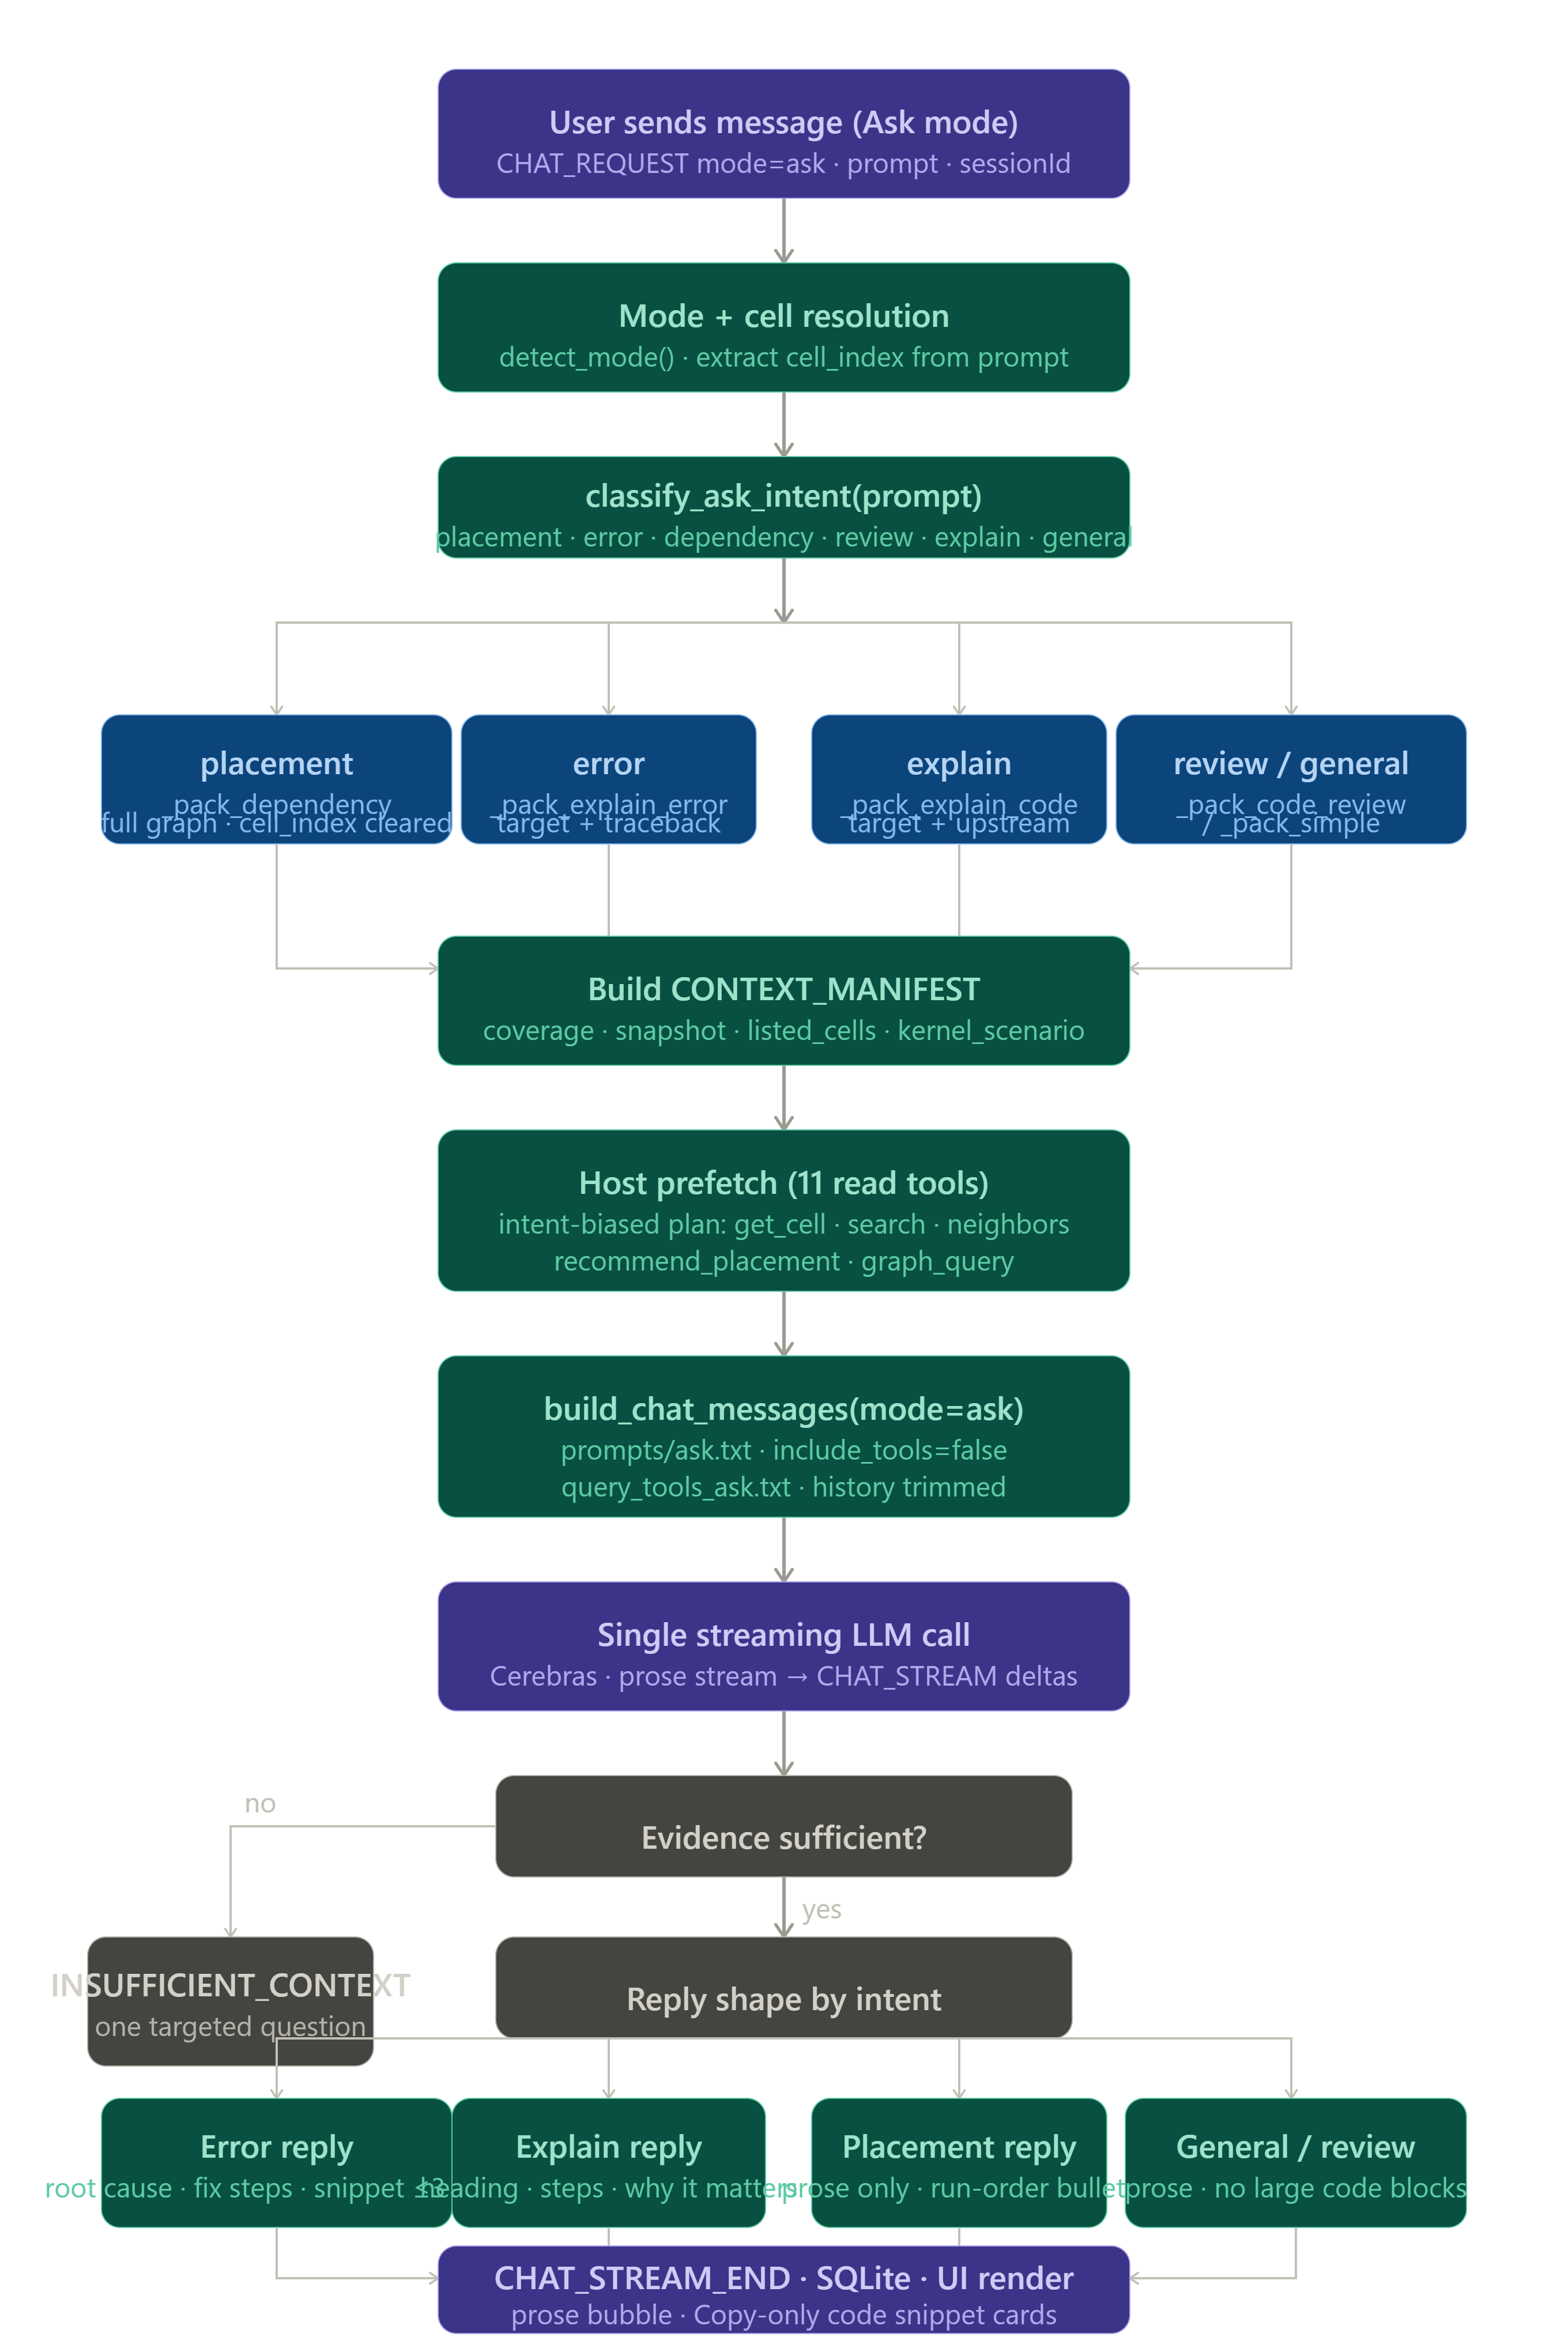
\includegraphics[width=0.95\textwidth]{ask_mode_advisory_flow.png}
\caption{Ask mode advisory flow (read-only explanation, no tool calls).}
\label{f-ask-flow}
\end{figure}

\subsection{Code mode}

Code mode loads \texttt{prompts/code.txt} and supports optional placement prefetch. Tools include \texttt{notebook\_recommend\_placement} and \texttt{notebook\_find\_symbol}. Replies are structured as Placement bullets followed by a single fenced \texttt{python} cell when generating code. Empty target cells trigger a clarification flow: the model acknowledges emptiness, asks intent, and defers full code until the user specifies a task---a pattern validated in Code benchmarks (Chapter~\ref{c-results}). Figure~\ref{f-code-flow} shows the Code mode generation flow.

\begin{figure}[!ht]
\centering
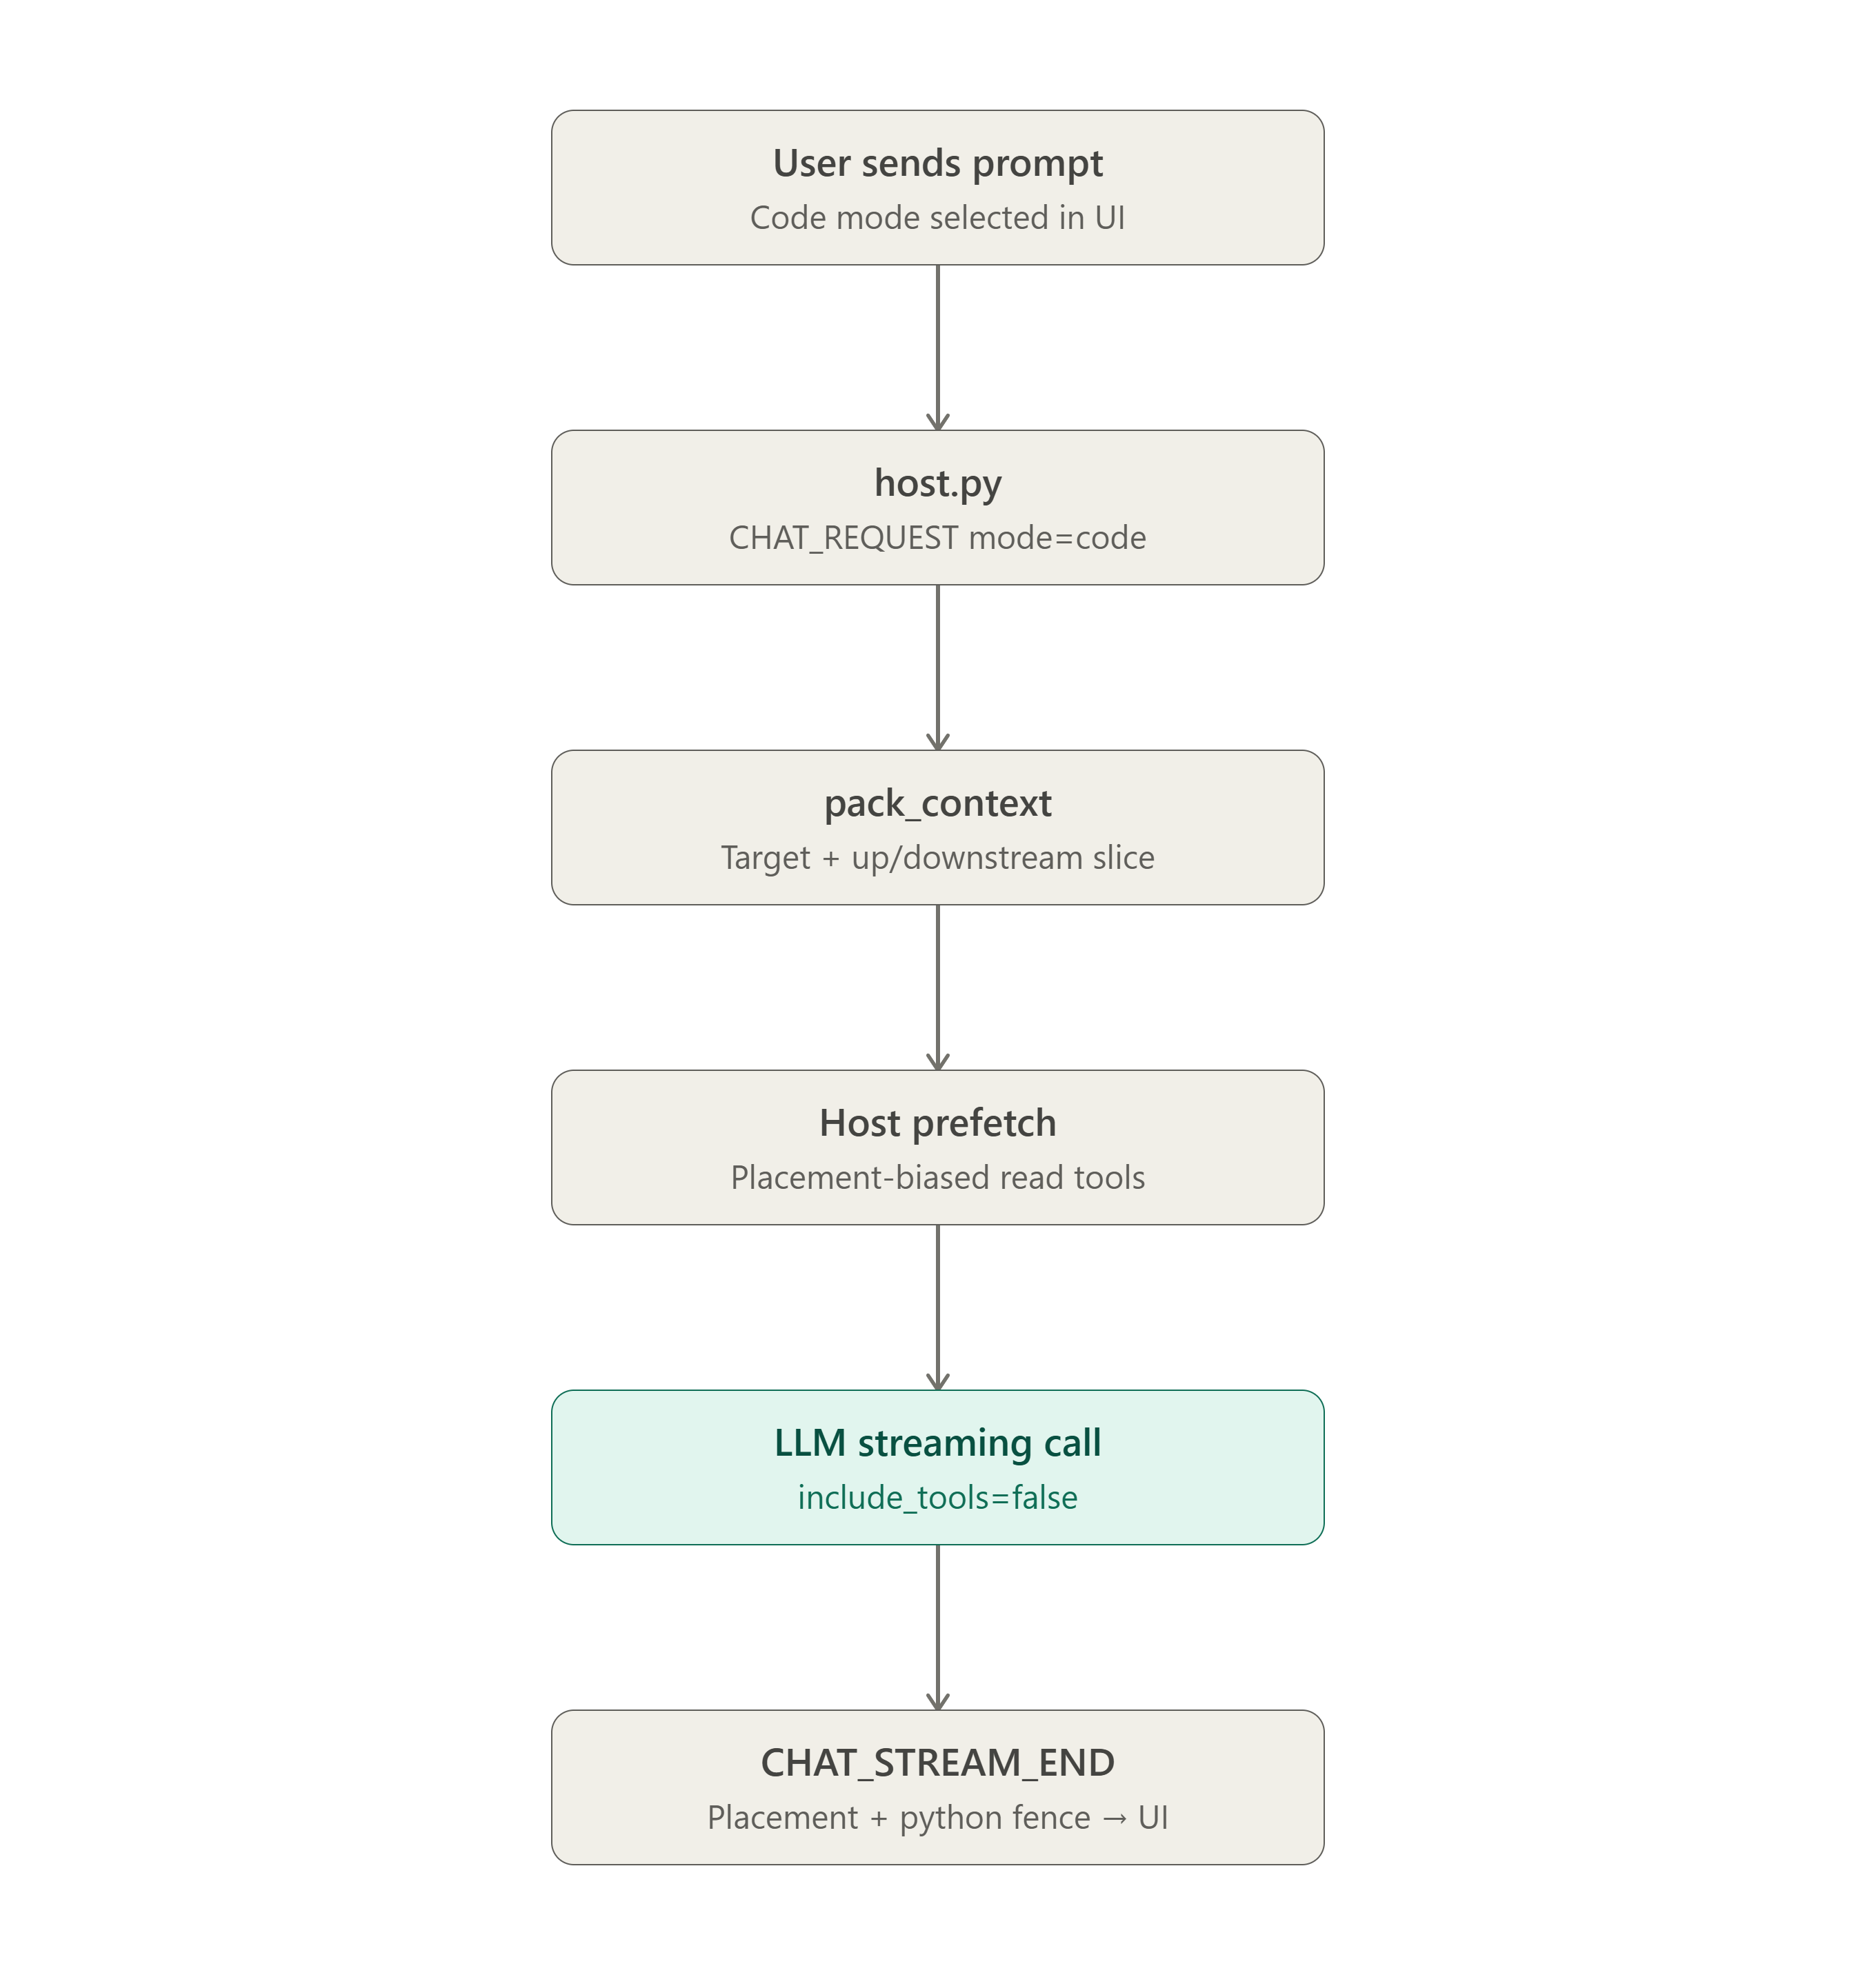
\includegraphics[width=0.95\textwidth]{code_mode_generation_flow.png}
\caption{Code mode generation flow (placement guidance and runnable cells, no browser writes).}
\label{f-code-flow}
\end{figure}

\subsection{Agentic mode}

Agentic mode loads \texttt{prompts/agentic.txt} plus tool-calling autogen descriptors. Each user message triggers exactly two \ac{API} completions when tools are enabled:

\begin{enumerate}
  \item \textbf{Round~0 (query).} The model may call local read tools only. Typical calls include \texttt{notebook\_list\_cells} and \texttt{notebook\_get\_cell}. Write tools are stripped by the phase guard.
  \item \textbf{Round~1 (implement).} The model emits the implement batch, including \texttt{insert\_cell}, \texttt{edit\_cell\_by\_index}, \texttt{delete\_by\_index}, and \texttt{run\_cell}. Redundant query tools are stripped. The host reorders bulk positional operations, then dispatches the batch in fire-and-forget mode.
\end{enumerate}

This protocol is \emph{not} a full ReAct loop \parencite{yao2023react}: the host does not feed per-cell execution results back into a third model turn within the same user message. Future work may add such a loop using scrape-based observers (Section~\ref{sec:future-react}). Figure~\ref{f-agentic-workflow} summarises the Agentic mode workflow.

\begin{figure}[!ht]
\centering
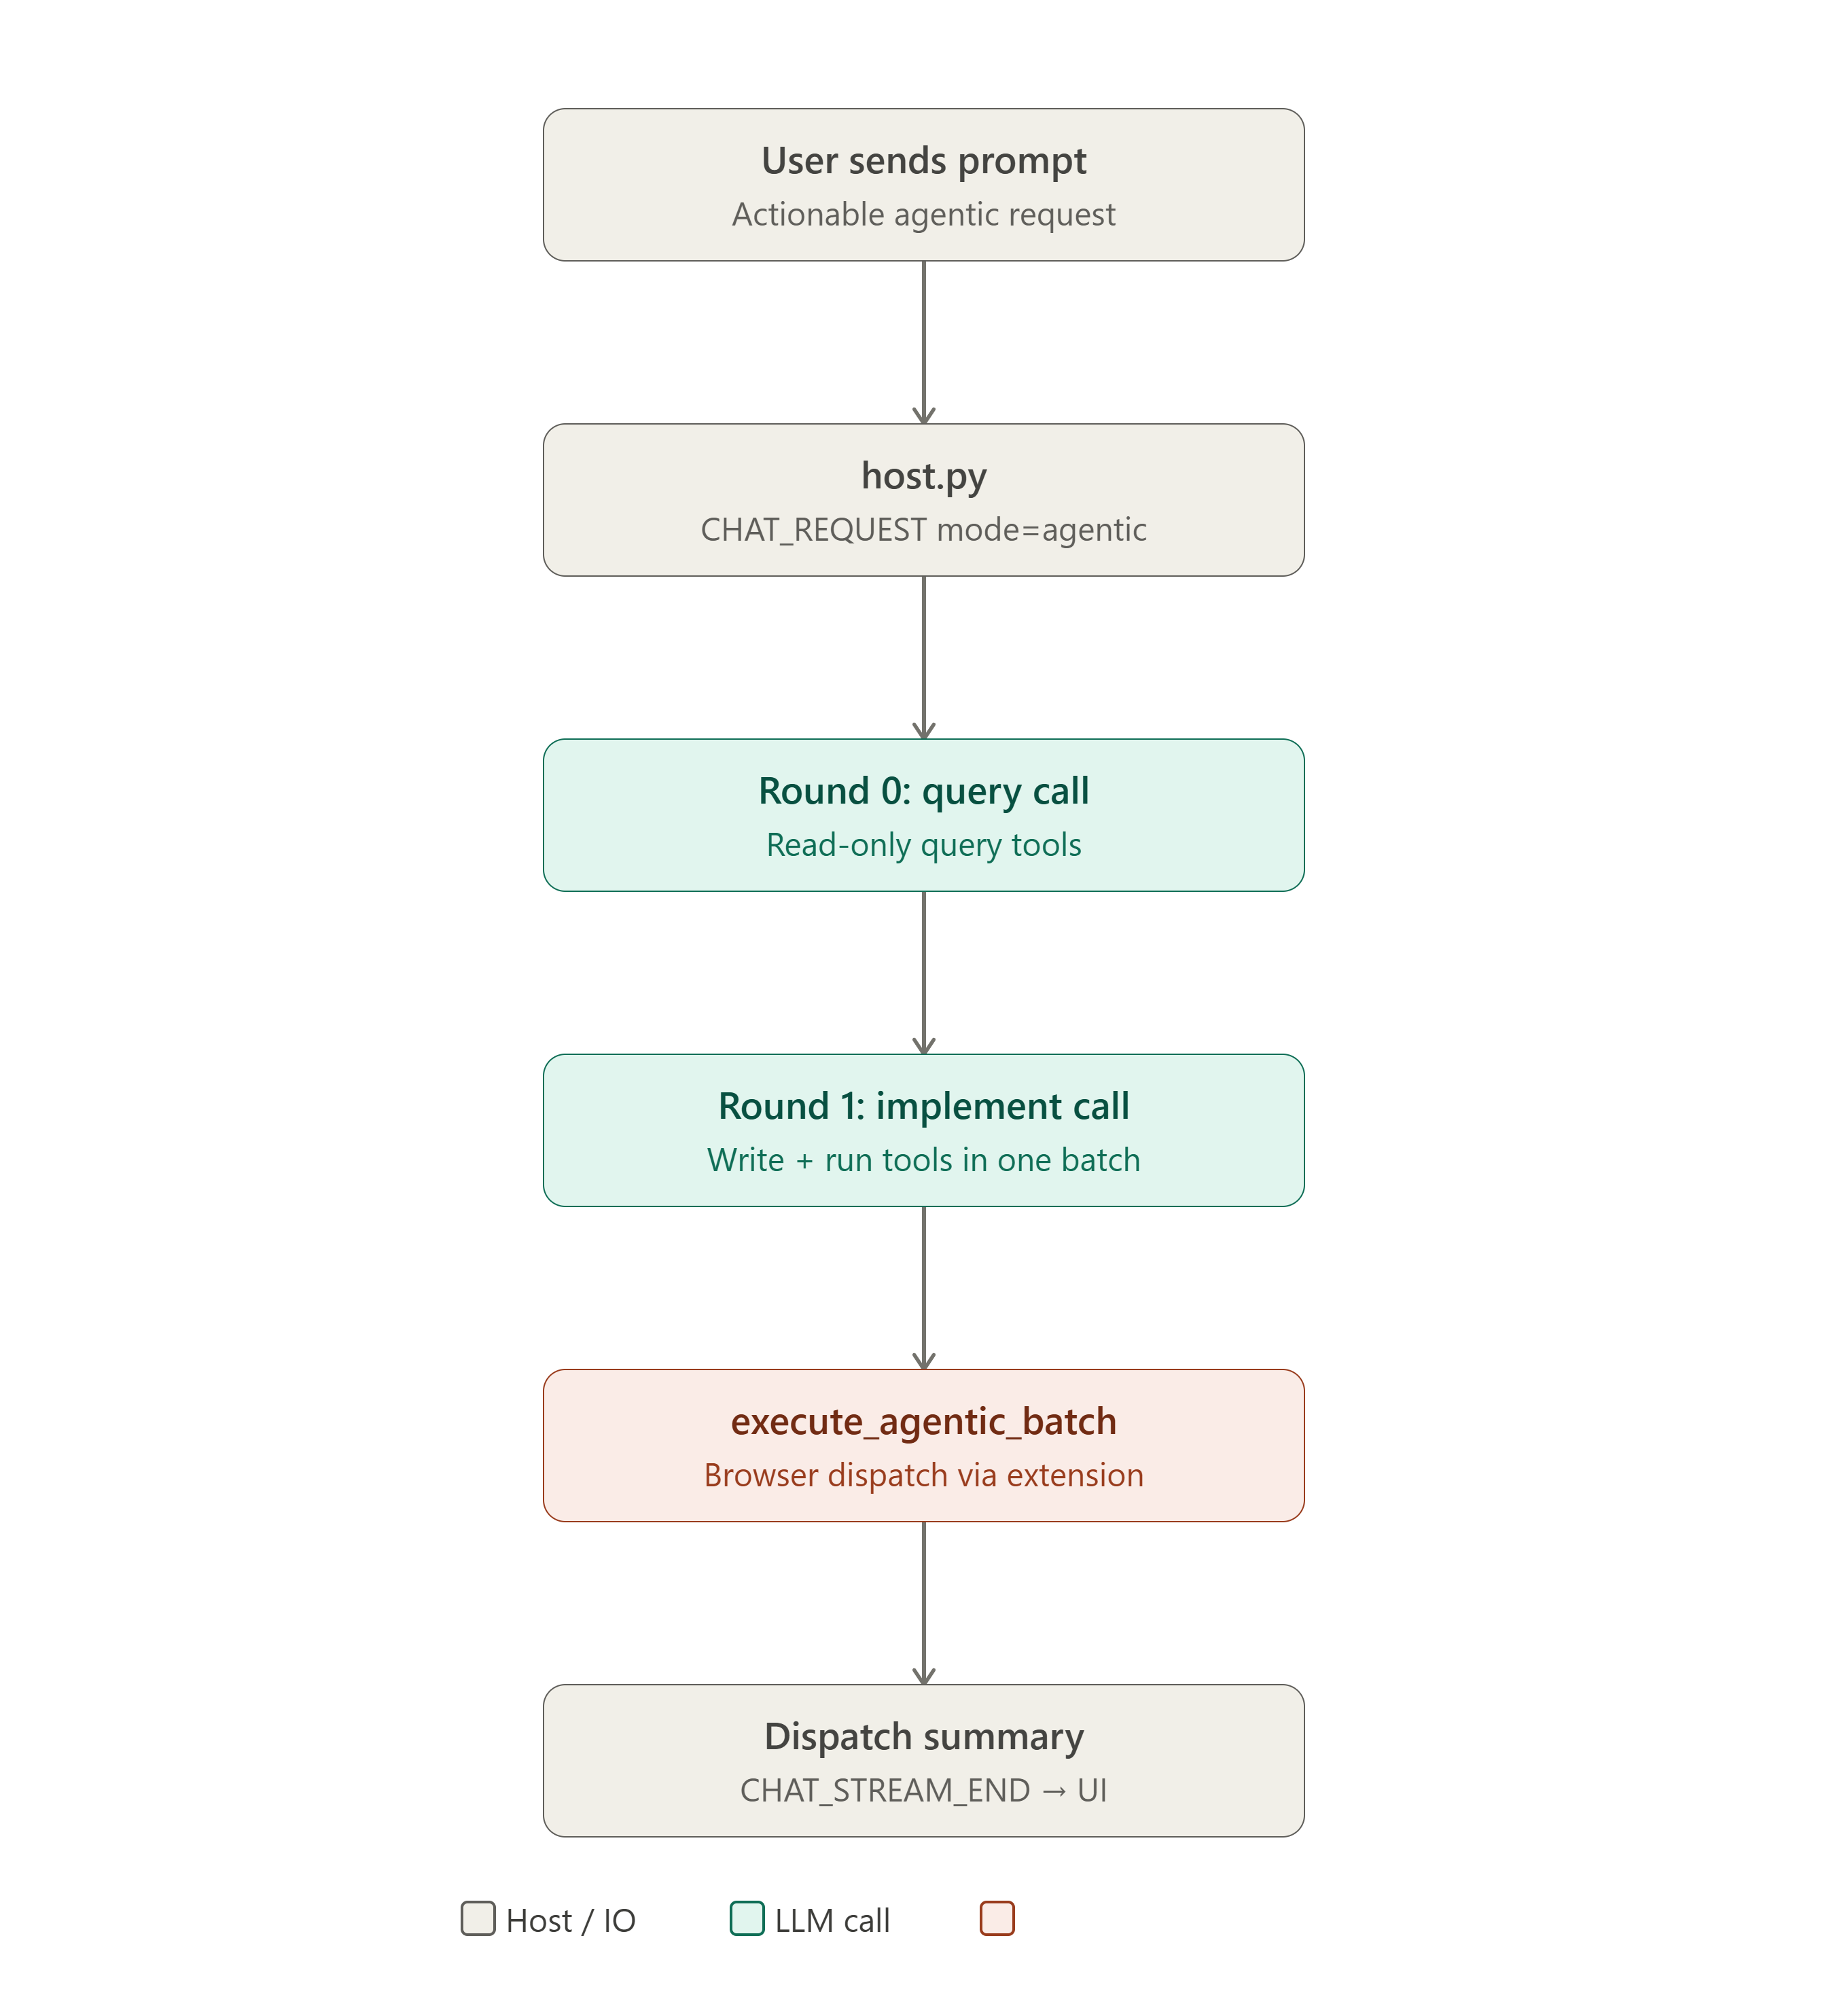
\includegraphics[width=0.95\textwidth]{agentic_mode_workflow.png}
\caption{Agentic mode workflow (two-phase query and implement with tool dispatch).}
\label{f-agentic-workflow}
\end{figure}

\section{Message Protocol and Session Lifecycle}
\label{sec:message-protocol}

Communication between extension and host uses typed JSON messages. Representative types include:

\begin{itemize}
  \item \texttt{CHAT\_REQUEST} --- user prompt, selected mode, \texttt{tab\_id}, notebook URL;
  \item \texttt{NOTEBOOK\_DATA} --- scraped cell list from extension;
  \item \texttt{INSERT\_CODE\_CELL}, \texttt{EDIT\_CELL\_BY\_INDEX}, \texttt{DELETE\_BY\_INDEX}, \texttt{RUN\_CELL} --- host-to-extension tool dispatches;
  \item \texttt{CHAT\_STREAM\_DELTA}, \texttt{CHAT\_STREAM\_END} --- streaming tokens to the user interface.
\end{itemize}

Session lifecycle for a single Agentic turn proceeds as follows:

\begin{enumerate}
  \item User selects Agentic mode and submits a prompt on a Kaggle \texttt{/edit} tab.
  \item Extension forwards \texttt{CHAT\_REQUEST} with \texttt{tab\_id} and URL; host resolves notebook storage key.
  \item Host packs context from live/persistent JSON and initiates round~0 completion with read tools.
  \item Local read tools execute against snapshots; results are appended to the message history.
  \item Host initiates round~1 completion; model returns parallel \texttt{tool\_calls}.
  \item Host validates arguments, applies phase guards, reorders batch, dispatches browser tools.
  \item Extension executes \ac{DOM} operations; results return asynchronously; trace logs record dispatch.
\end{enumerate}

Session keys (\texttt{kaggle:kernel:<id>}) align chat history, snapshot filenames, and tool arguments, preventing cross-notebook contamination when users switch tabs \parencite{lewis2020rag}.

\section{Implementation Phases}
\label{sec:impl-phases}

Table~\ref{tab:phases} maps development phases to deliverables. Each phase concluded with targeted tests under \texttt{testing/host/tests/}.

\begin{table}[!ht]
\centering
\caption{Implementation phases and deliverables.}
\label{tab:phases}
\small
\begin{tabular}{|c|p{4.2cm}|p{6.8cm}|}
\hline
\textbf{Phase} & \textbf{Focus} & \textbf{Deliverable} \\ \hline
1 & \ac{DOM} scrape and snapshot ingest & Extension scrape pipeline; \texttt{notebook\_data\_handler.py} \\ \hline
2 & Native messaging and host I/O & \texttt{host.py} dispatcher; Chrome host manifest \\ \hline
3 & Ask/Code streaming chat & \texttt{streaming.py}; mode prompts \\ \hline
4 & Tool registry and browser dispatch & Six browser tools; session coercion \\ \hline
5 & Agentic two-phase batching & Phase guards; \texttt{agentic\_batch\_executor.py} \\ \hline
6 & Benchmark harness and evaluation & \texttt{run\_*\_tests.py}; trace metrics \\ \hline
\end{tabular}
\end{table}

\section{Registered Tools}
\label{sec:tools-table}

Table~\ref{tab:tools} lists tools exposed to the model in Agentic mode.

\begin{table}[!ht]
\centering
\caption{Registered notebook tools.}
\label{tab:tools}
\small
\begin{tabular}{|p{3.6cm}|p{2.2cm}|p{6.8cm}|}
\hline
\textbf{Tool} & \textbf{Executor} & \textbf{Purpose} \\ \hline
\texttt{notebook\_list\_cells} & Host (local) & Enumerate cells with indices and types \\ \hline
\texttt{notebook\_get\_cell} & Host (local) & Fetch source/output for one index \\ \hline
\texttt{insert\_cell} & Browser & Insert code/markdown at position \\ \hline
\texttt{edit\_cell\_by\_index} & Browser & Replace cell source \\ \hline
\texttt{delete\_by\_index} & Browser & Remove cell at index \\ \hline
\texttt{run\_cell} & Browser & Execute cell in kernel \\ \hline
\end{tabular}
\end{table}

Tool schemas are generated from \texttt{prompts/tool\_calling/} autogen files, keeping documentation synchronized with the registry \parencite{qin2024toolllm,li2023apibank}.

\subsection{Detailed benchmark scenarios}
\label{sec:benchmark-scenarios}

\textbf{Ask suite.} (1)~Explain full notebook workflow; (2)~explain cell~17; (3)~diagnose error in cell~31. Metrics: topic coverage, evidence alignment, hallucination heuristic; contract: zero tools and zero writes.

\textbf{Code suite.} (1)~XGBoost pipeline cell; (2)~replace cell~21 preprocessing; (3)~feature-engineering module; (4)~empty-cell workflow. Metrics: code correctness, placement accuracy; contract: zero browser writes.

\section{Data Flow for a Single User Turn}
\label{sec:data-flow}

Figure~\ref{f-dataflow} summarises the message sequence for Agentic mode. Ask and Code modes omit round~1 tool dispatch but share the scrape-and-pack path.

\begin{figure}[!ht]
\centering
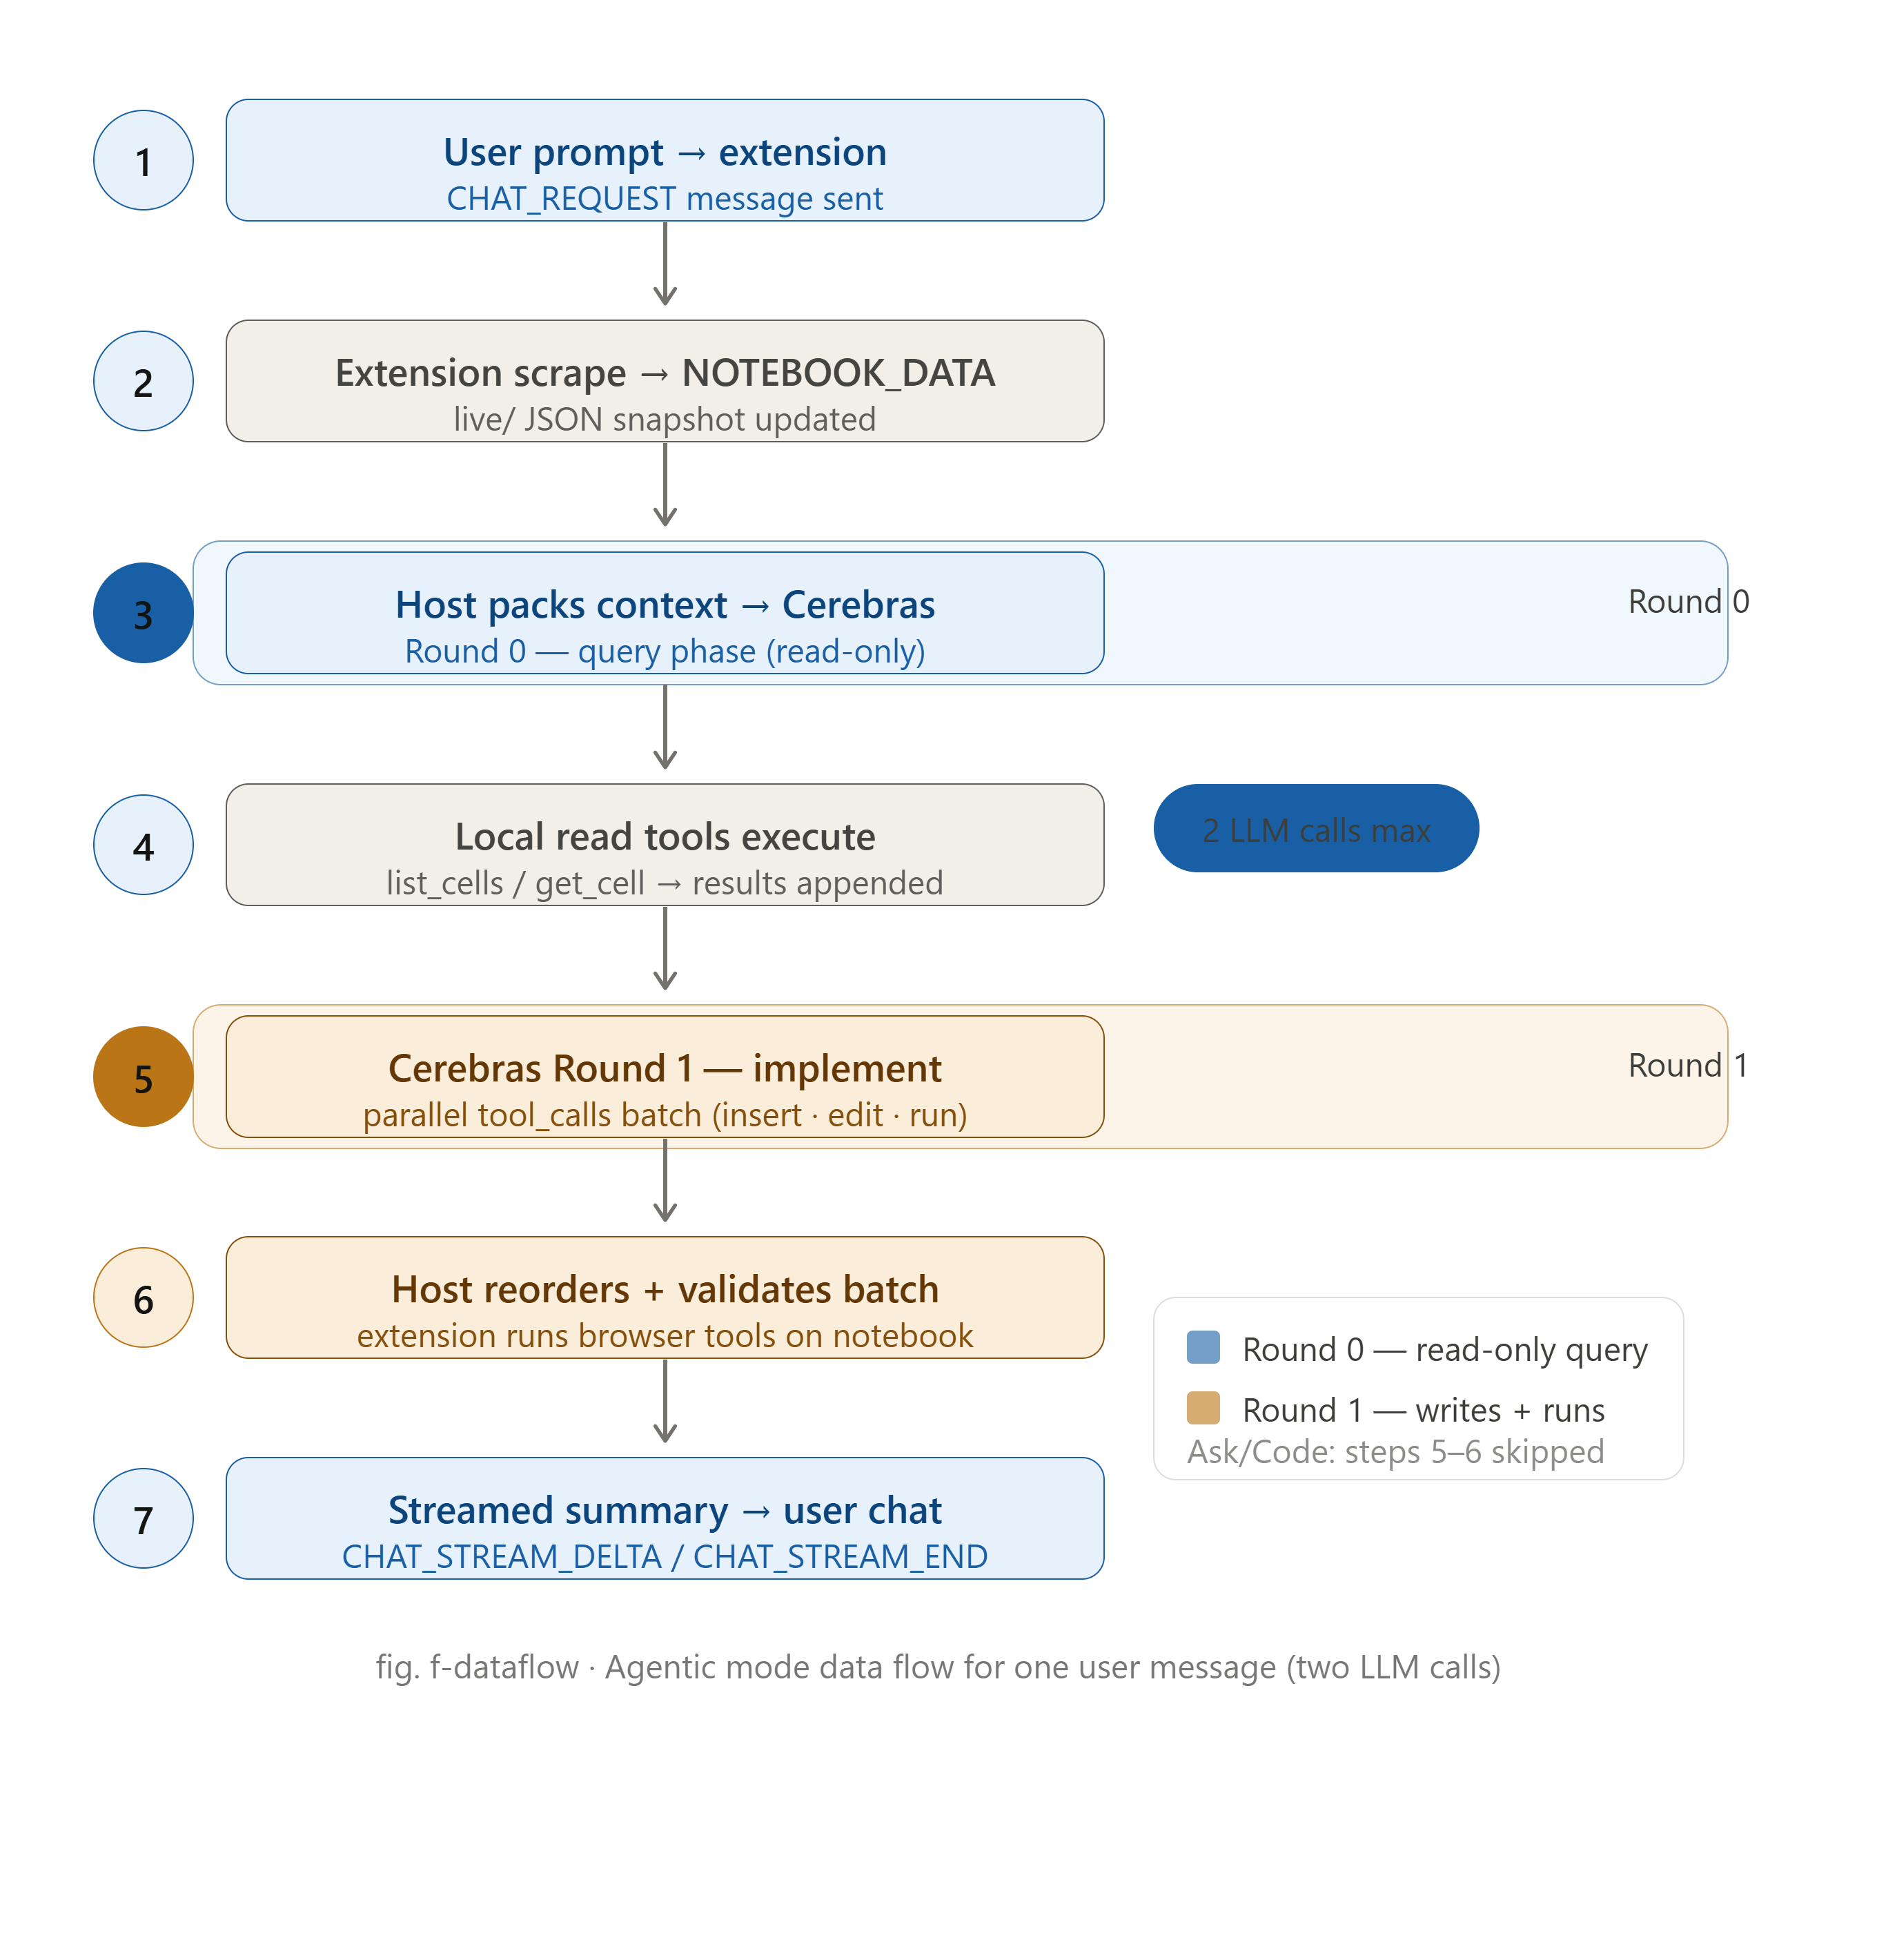
\includegraphics[width=0.95\textwidth]{f_dataflow_agentic.png}
\caption{Agentic mode data flow for one user message (two LLM calls).}
\label{f-dataflow}
\end{figure}

\subsection{Snapshot schema}

Each cell object in the JSON snapshot typically contains:

\begin{itemize}
  \item \texttt{index} --- positional label aligned with tool arguments;
  \item \texttt{type} --- \texttt{code} or \texttt{markdown};
  \item \texttt{source} --- cell input text;
  \item \texttt{outputs} --- optional list of stdout/stderr/display data when scraped;
  \item \texttt{execution\_count} --- optional prompt number when visible in the \ac{DOM}.
\end{itemize}

The host strips or retains execution metadata according to flag {\ttfamily\seqsplit{KERNEL\_EXECUTION\_METADATA\_ENABLED}}, balancing token budget against diagnostic value for Ask mode error explanation.

\subsection{Token budgeting}

Context packing applies two limits. {\ttfamily\seqsplit{MAX\_INPUT\_TOKENS}} caps the full message list; {\ttfamily\seqsplit{MAX\_NOTEBOOK\_CONTEXT\_CHARS}} caps the notebook slice. When limits are exceeded, older chat history is truncated first; notebook cells are packed from the start of the document unless intent-based packing selects a window around a cited cell index. This policy explains workflow-level Ask behaviour on long notebooks discussed in Chapter~\ref{chap:discussion}.

\section{Security and Trust Model}
\label{sec:security}

The trust model assigns capabilities to each component:

\begin{itemize}
  \item \textbf{Extension.} Same-origin \ac{DOM} access on Kaggle pages the user has opened; no network egress except native messaging and Kaggle itself.
  \item \textbf{Host.} Holds \ac{API} credentials; reads/writes local snapshot files; dispatches tool commands only to the connected extension port.
  \item \textbf{Remote model.} Receives prompts and tool schemas; does not receive browser cookies or Kaggle authentication tokens.
\end{itemize}

Tool argument validation rejects out-of-range cell indices and malformed JSON before dispatch. Session coercion overwrites model-supplied URLs with the canonical notebook URL from the active turn, reducing the risk of cross-tab misrouting when the model hallucinates a different kernel link.

\section{Testing and Quality Assurance}
\label{sec:qa}

Quality assurance combined unit tests, smoke scripts, and benchmark suites:

\begin{itemize}
  \item \textbf{Unit tests} (\texttt{testing/host/tests/}) cover cell indexing, batch reordering, phase guards, and tool-chain parsing.
  \item \textbf{Smoke scripts} (\texttt{smoke\_*.py}) exercise individual browser tools against mock or live sessions.
  \item \textbf{Monitor scripts} (\texttt{monitor\_*.py}) observe cell additions and kernel execution during manual testing.
  \item \textbf{Benchmark suites} provide reproducible mode-contract evaluation documented in Appendix~\ref{app:benchmarks}.
\end{itemize}

Regression failures in phase guards or index coercion were treated as release blockers because they directly threaten notebook integrity---a lesson consistent with notebook best-practice literature emphasising reproducible execution order \parencite{rule2019tenrules}.

\chapter{Results}
\label{c-results}

So show what you did so far (implementation and testing) that is relevant to
answering the question(s) or solving the problem(s).

%!TEX root = ../_fyp.tex
\chapter{Discussion}
\label{chap:discussion}

Chapter~\ref{c-results} established that Ask, Code, and Agentic modes satisfy distinct contracts on shared notebook snapshots. This chapter interprets those findings relative to prior work on notebook assistants \parencite{mcnutt2023notebookassistants,rule2018exploration}, tool-augmented \acp{LLM} \parencite{schick2023toolformer,qin2024toolllm}, and interactive programming cost models \parencite{mozannar2024reading}.

\section{Agentic Tool Dispatch}

The primary Agentic result---37 tools dispatched in the second \ac{API} call after a read-only query round---confirms that GLM~4.7 can emit large parallel \texttt{tool\_calls} batches when native tool schemas are attached \parencite{qin2024toolllm}. The two-call design trades the flexibility of open-ended ReAct trajectories \parencite{yao2023react} for predictable latency and cost, consistent with fire-and-forget batching described in Section~\ref{sec:tool-registry}.

Importantly, the present artefact \emph{does not} close the loop with per-cell observation and replanning. Dispatch success therefore indicates planning fidelity at the host boundary, not guaranteed kernel outcomes in the live editor. This distinction aligns with \textcite{hou2024llm4se}, who note that software-engineering agents require explicit evaluation criteria matched to deployment contracts. For the FYP, dispatch-only scoring is the appropriate metric until a future ReAct implementation is added (Section~\ref{sec:future-react}).

Host-side descending reorder for bulk inserts and deletes mitigated index-shift risk identified in notebook integration literature \parencite{rule2019tenrules,chasins2018roussillon}. The Pakistan housing pipeline batch suggests that domain-specific tool narrowing---six vetted cell operations rather than open web APIs \parencite{patil2023gorilla}---improves batch coherence.

\section{Ask Mode: Explanation Without Side Effects}

Ask mode achieved strong performance on cell-local explanation (cell~17) and error diagnosis (cell~31) while maintaining zero side effects. Zero tool calls eliminate the verification burden that \textcite{vaithilingam2022expectation} associate with generative coding tools, because the assistant cannot mutate the artefact under discussion.

The notebook workflow test exhibited 89\% topic coverage, indicating that the model recognised standard data-science stages (loading, cleaning, feature work, modelling, evaluation) from packed context---a form of lightweight retrieval grounding \parencite{lewis2020rag}. The remaining limitation is depth: without full notebook coverage in the prompt window \parencite{wei2022chain,brown2020language}, workflow answers may summarise stages rather than exhaustively trace every cell. This is an expected trade-off for closed-platform assistants that lack platform \ac{API} access \parencite{chasins2018roussillon}.

For educational use in \acf{BSDS} coursework, Ask mode is best positioned as a \emph{read-only tutor}: explain cells, diagnose errors, and clarify intent before the student authors or runs code \parencite{finnieansley2022codex}.

\section{Code Mode: Implementation Guidance}

Code mode passed all four reported scenarios while preserving the no-write contract. Correct XGBoost training code (100\% keyword alignment with notebook variables) shows that snapshot grounding suffices for variable reuse without live kernel introspection \parencite{lewis2020rag}. Cell replacement and feature-engineering tests further indicate that the model can emit self-contained cells matching notebook naming conventions \parencite{wang2021welldocumented}.

The empty-cell workflow result---asking intent before emitting Placement and Code sections---implements the deferral pattern recommended for notebook copilots \parencite{mcnutt2023notebookassistants} and reduces the risk of unsolicited code dumps \parencite{mozannar2024reading}.

The principal weakness is placement accuracy under partial context: correct code may be paired with suboptimal insert indices. This mirrors IDE copilot findings that suggestion quality depends on visible context \parencite{ziegler2024copilot}, extended to positional notebook cells rather than flat files.

\section{Mode Selection Implications}

Table~\ref{tab:mode-guidance} translates results into practical guidance. The separation supports Objective~6 in Section~\ref{sec:objectives}: empirical validation across modes, not a single monolithic assistant score.

\begin{table}[!ht]
\centering
\caption{Practical mode selection guidance derived from benchmarks.}
\label{tab:mode-guidance}
\small
\begin{tabular}{|p{3.2cm}|p{4.2cm}|p{4.8cm}|}
\hline
\textbf{User goal} & \textbf{Recommended mode} & \textbf{Evidence} \\ \hline
Understand notebook or cell & Ask & 89\% workflow coverage; 0\% hallucination on cell~17 \\
Diagnose execution error & Ask & Correct root-cause on cell~31 \\
Implement new cell safely & Code & Runnable blocks; 0 browser writes \\
Automate multi-cell batch & Agentic & 37-tool dispatch after query call \\ \hline
\end{tabular}
\end{table}

\section{Threats to Validity}

Three threats qualify the generalisability of findings. \textbf{Harness fidelity:} Agentic tests mock browser execution; traces record dispatch, not live Kaggle latency. \textbf{Heuristic scoring:} Coverage and code-correctness metrics automate keyword rubrics rather than expert judgment \parencite{chen2021codex}. \textbf{Single-model scope:} All runs use GLM~4.7; cross-model replication would strengthen claims \parencite{hou2024llm4se}. Despite these limits, the benchmarks provide reproducible evidence that mode contracts are enforceable in a deployable Chrome extension architecture.

\section{Comparison with Prior Notebook Assistants}
\label{sec:comparison-prior}

\textcite{mcnutt2023notebookassistants} prototyped inline suggestions within JupyterLab-style environments where extension APIs expose cell metadata directly. The present artefact operates on Kaggle's closed \texttt{/edit} surface without platform cooperation, trading API richness for \ac{DOM} scraping \parencite{chasins2018roussillon}. Relative to their design probes, this FYP adds three distinctions:

\begin{itemize}
  \item \textbf{Explicit mode contracts} separate read-only tutoring (Ask), copy-paste generation (Code), and batched dispatch (Agentic) rather than a single inline suggestion channel.
  \item \textbf{Native tool calling} replaces free-form code fences with schema-validated \texttt{insert\_cell} and \texttt{run\_cell} operations \parencite{qin2024toolllm}.
  \item \textbf{Host-side batch reordering} addresses positional index shift---a notebook-specific hazard absent in flat-file copilots \parencite{rule2019tenrules}.
\end{itemize}

IDE copilots such as GitHub Copilot excel at file-buffer completion \parencite{ziegler2024copilot} but do not model markdown/code interleaving or kernel execution order. The benchmark evidence suggests that notebook assistance requires platform-specific grounding even when the underlying model is shared.

\section{Educational Implications for BSDS}
\label{sec:edu-implications}

For \acf{BSDS} coursework at \acf{GCUF}, the mode separation maps onto pedagogical stages:

\begin{enumerate}
  \item \textbf{Exploration phase.} Students use Ask mode to understand forked Kaggle kernels before editing---mirroring \textcite{rule2018exploration}'s distinction between exploration and explanation notebooks.
  \item \textbf{Implementation phase.} Code mode supports assessed assignments where students must author cells themselves but benefit from placement hints and runnable templates \parencite{finnieansley2022codex}.
  \item \textbf{Automation phase.} Agentic mode demonstrates how tool-augmented models plan multi-cell workflows, preparing advanced students for agentic data-science tooling while remaining bounded by the two-call contract.
\end{enumerate}

The empty-cell deferral results (Code Test~4) are particularly relevant: assistants should clarify intent before filling cells in graded work, reducing academic integrity concerns associated with unsolicited code dumps \parencite{vaithilingam2022expectation}.

\section{Architectural Trade-offs}
\label{sec:arch-tradeoffs}

The split extension--host design embodies deliberate trade-offs summarised in Table~\ref{tab:tradeoffs}.

\begin{table}[!ht]
\centering
\caption{Architectural trade-offs in the implemented system.}
\label{tab:tradeoffs}
\small
\begin{tabular}{|p{3.4cm}|p{4.8cm}|p{4.8cm}|}
\hline
\textbf{Decision} & \textbf{Benefit} & \textbf{Cost} \\ \hline
Native messaging & API keys never in extension; full-duplex I/O & Local install and host registration \\ \hline
DOM scraping & Works without Kaggle API & Fragile to front-end changes \\ \hline
Two-call Agentic cap & Predictable latency and billing & No mid-batch replanning \\ \hline
Fire-and-forget dispatch & High throughput (37 tools in one batch) & No execution verification in same turn \\ \hline
Dual JSON stores & Fresh live + durable persistent context & Storage sync complexity \\ \hline
\end{tabular}
\end{table}

These trade-offs reflect FYP scope constraints (Section~\ref{sec:scope}) while remaining transferable to other closed notebook platforms identified in Chapter~\ref{c-review}.

\section{Context Packing as a Cross-Mode Bottleneck}
\label{sec:context-bottleneck}

Ask Test~1 and Code placement limitations share a root cause: the host packs notebook context subject to \texttt{MAX\_NOTEBOOK\_CONTEXT\_CHARS} and \texttt{MAX\_INPUT\_TOKENS}. Long competition notebooks exceed single-window coverage \parencite{wei2022chain}. The model's appropriate response---high-level workflow summary rather than per-cell invention---is pedagogically sound but reduces automated accuracy scores.

Mitigations proposed in Section~\ref{sec:future-react} include hierarchical section summaries and retrieval over cell embeddings \parencite{lewis2020rag,jiang2023structgpt}. Until implemented, practitioners should prefer cell-local Ask queries and verify Code placement against the visible editor.

\section{Reliability and Safety Posture}
\label{sec:safety}

From a safety perspective, mode contracts provide defence in depth:

\begin{itemize}
  \item Ask mode cannot mutate notebooks---eliminating accidental destructive edits during explanation.
  \item Code mode requires explicit user copy-paste---preserving human approval before execution.
  \item Agentic mode batches all writes in one host-validated queue---enabling user review of planned operations before browser execution completes.
\end{itemize}

This posture aligns with \textcite{mozannar2024reading}'s finding that users accept AI assistance when edit semantics are predictable. Future ReAct loops must preserve these guardrails rather than bypassing them for autonomy \parencite{shinn2023reflexion}.

%!TEX root = ../_fyp.tex
\chapter{Conclusion}
\label{cha:conclusion}

This FYP set out to build an agentic \ac{LLM} assistant that grounds reasoning in live Kaggle notebook state and manipulates cells through a bounded tool interface. The implemented system---a Chrome extension, Python native host, dual JSON snapshot stores, and GLM~4.7 integration via Cerebras---addresses the context-grounding and tool-mediation problems stated in Section~\ref{sec:problem-statement}.

\section{Summary of Findings}

\textbf{Architecture.} The extension--host split enforces a clear trust boundary: \ac{DOM} access and tool execution remain in the browser; \ac{API} credentials and orchestration remain on the host \parencite{chasins2018roussillon,qin2024toolllm}. Session keys derived from Kaggle kernel identifiers align snapshots, chat history, and tool arguments.

\textbf{Agentic mode.} Under the mandatory two-call contract, the model first queries notebook structure and then dispatches an implement batch. The reported ML pipeline test achieved successful dispatch of 37 tools (24 insert, 24 edit, 24 run, 2 read) in the second \ac{API} call. This demonstrates feasible batch planning for multi-cell workflows without an open ReAct loop \parencite{yao2023react}.

\textbf{Ask mode.} Read-only assistance achieved strong cell-level explanation (0\% heuristic hallucination on cell~17), reliable error diagnosis on cell~31, and 89\% workflow topic coverage on the notebook explanation task---all with zero tool calls and zero writes.

\textbf{Code mode.} All four reported scenarios passed under the no-write contract, including correct XGBoost training code, cell replacement, feature-engineering modules, and empty-cell intent deferral \parencite{mcnutt2023notebookassistants}.

\section{Research Objectives Revisited}

Objectives~1--5 (architecture, context pipeline, tools, agentic contract, scrape-based monitors) were realised in the artefact described in Chapter~\ref{c-methods}. Objective~6 (empirical validation) was addressed through the three benchmark suites in Chapter~\ref{c-results}. The evidence supports the hypothesis that \emph{mode-specific contracts}---Ask for understanding, Code for implementation guidance, Agentic for batched dispatch---produce measurably different behaviour on the same notebook corpus.

\section{Contributions}

Relative to generic chat interfaces and IDE copilots \parencite{ziegler2024copilot,vaithilingam2022expectation}, this work contributes: (i)~DOM-grounded notebook snapshots for a closed web editor; (ii)~a vetted six-tool surface for positional cell operations; (iii)~a mandatory query--implement two-call Agentic protocol with host-side batch reordering; and (iv)~an reproducible evaluation harness distinguishing dispatch fidelity from execution verification.

\section{Future Work}
\label{sec:future-react}

The current Agentic mode deliberately omits a full ReAct-style observe--act loop with per-cell feedback \parencite{yao2023react,shinn2023reflexion}. A natural extension is to add replanning rounds that ingest execution traces from scrape-based monitors (Section~\ref{sec:tool-registry}), enabling goal verification after each \texttt{run\_cell}. Additional directions include: retrieval-augmented packing for long notebooks \parencite{lewis2020rag,jiang2023structgpt}; live Kaggle \ac{DOM} studies to complement harness results; and cross-model evaluation \parencite{hou2024llm4se,openai2023gpt4}.

In sum, the project demonstrates that a deployable notebook copilot can separate explanation, code generation, and tool orchestration into three modes while sharing a common grounding pipeline---a design pattern applicable beyond Kaggle to other closed notebook platforms identified in Chapter~\ref{c-review}.

\section{Lessons Learned}
\label{sec:lessons}

Development of the artefact yielded four practical lessons for future notebook-agent projects:

\begin{enumerate}
  \item \textbf{Positional identity is first-class.} Tool arguments must use the same indexing convention as the scraped \ac{DOM}; mismatches between zero-based and one-based indices were a recurring integration bug during Phase~4 (Table~\ref{tab:phases}).
  \item \textbf{Phase guards are essential.} Without stripping write tools in round~0, models occasionally emitted premature inserts before reading notebook structure---violating the query--implement discipline advocated in agentic literature \parencite{yao2023react}.
  \item \textbf{Batch reordering prevents index drift.} Descending-order deletes and inserts materially reduced failed dispatches in multi-cell Agentic tests compared with naive queue order.
  \item \textbf{Evaluation must match implementation.} Scoring Agentic runs on verification criteria the host does not implement would misrepresent system capability; dispatch-only metrics align claims with the shipped artefact.
\end{enumerate}

\section{Alignment with Research Objectives}

Table~\ref{tab:objective-map} maps each objective from Section~\ref{sec:objectives} to evidence in this dissertation.

\begin{table}[!ht]
\centering
\caption{Research objectives and supporting evidence.}
\label{tab:objective-map}
\small
\begin{tabular}{|c|p{4.2cm}|p{5.8cm}|}
\hline
\textbf{Obj.} & \textbf{Topic} & \textbf{Evidence} \\ \hline
1 & Architecture & Ch.~\ref{c-methods}, Fig.~\ref{f-architecture}; extension--host split \\ \hline
2 & Context pipeline & \ref{sec:notebook-json}; dual live/persistent stores \\ \hline
3 & Tool operations & \ref{sec:tools-table}; six registered tools \\ \hline
4 & Agentic contract & Test~1: 37-tool batch in 2 calls \\ \hline
5 & Scrape monitors & \texttt{cell\_execution\_observer.py} \\ \hline
6 & Empirical validation & Ch.~\ref{c-results}; three benchmark suites \\ \hline
\end{tabular}
\end{table}

All six objectives were addressed within stated scope limitations (Section~\ref{sec:limitations}).

%!TEX root = ../_fyp.tex
\chapter{Recommendations}
\label{c-recommendation}

Based on the implementation experience and benchmark outcomes in Chapters~\ref{c-results} and~\ref{chap:discussion}, we offer recommendations for practitioners, system maintainers, and future researchers.

\section{Recommendations for Practitioners}

Students and data-science practitioners using Kaggle notebooks should select the interaction mode that matches task risk and intent:

\begin{itemize}
  \item Use \textbf{Ask mode} to understand unfamiliar notebooks, explain individual cells, or diagnose errors before editing. Benchmarks showed zero side effects and strong cell-level accuracy \parencite{vaithilingam2022expectation}.
  \item Use \textbf{Code mode} when ready to copy runnable cells into the editor. Verify placement suggestions against notebook flow before inserting \parencite{mcnutt2023notebookassistants}.
  \item Use \textbf{Agentic mode} for large batched edits when willing to review dispatched operations. The two-call protocol plans writes and runs together; users should inspect the batch before relying on outcomes \parencite{mozannar2024reading}.
\end{itemize}

For empty cells, prefer Ask or Code mode clarifying questions over immediate code generation. In evaluation, both modes deferred full scripts until intent was clear.

\section{Recommendations for System Improvement}

\begin{enumerate}
  \item \textbf{Implement ReAct-style feedback.} Add optional replanning after \texttt{run\_cell} using scrape-based execution observers, closing the gap between dispatch-only Agentic mode and full autonomous repair \parencite{yao2023react,shinn2023reflexion}.
  \item \textbf{Expand context packing.} Adopt hierarchical or retrieval-augmented cell selection for long notebooks to improve workflow-level Ask answers and Code placement \parencite{lewis2020rag,jiang2023structgpt}.
  \item \textbf{Harden DOM selectors.} Maintain scrape utilities against Kaggle front-end changes, following lessons from web data extraction research \parencite{chasins2018roussillon}.
  \item \textbf{Add human evaluation.} Supplement automated rubrics with expert grading for explanation quality and code correctness \parencite{chen2021codex,wang2021welldocumented}.
  \item \textbf{Live browser benchmarks.} Replicate harness scenarios on actual \texttt{/edit} sessions to measure end-to-end latency and user-perceived trust \parencite{mozannar2024reading}.
\end{enumerate}

\section{Recommendations for Future Research}

\begin{itemize}
  \item Compare GLM~4.7 with additional code models \parencite{openai2023gpt4,brown2020language} on identical frozen snapshots.
  \item Study learning outcomes when \acf{BSDS} students use Ask versus Code versus Agentic assistance during coursework \parencite{finnieansley2022codex}.
  \item Explore narrower tool APIs inspired by API-bank and Gorilla benchmarks \parencite{li2023apibank,patil2023gorilla} tailored to competition notebooks \parencite{quaranta2022bestpractices}.
  \item Investigate session-level memory across turns to reduce repeated query rounds in Agentic mode \parencite{park2023generative}.
\end{itemize}

These recommendations preserve the current system's strengths: grounded context, mode separation, and bounded Agentic dispatch. They also identify clear paths toward fuller autonomous notebook assistance in future iterations.

\section{Deployment and Maintenance Checklist}
\label{sec:deploy-checklist}

Teams deploying or extending the artefact should complete the following steps:

\begin{enumerate}
  \item Install the Chrome extension in developer mode and register the native host manifest (\texttt{register.ps1}).
  \item Configure \texttt{CEREBRAS\_API\_KEY} and \texttt{CEREBRAS\_MODEL} in \texttt{testing/host/.env}.
  \item Verify native messaging connectivity by opening a Kaggle \texttt{/edit} tab and sending an Ask-mode query.
  \item Enable Agentic mode only after confirming snapshot ingestion (\texttt{data/notebooks/live/} updates on scrape).
  \item Run smoke scripts under \texttt{testing/host/scripts/} after any \ac{DOM} selector change.
  \item Re-execute benchmark suites before thesis or demo updates (Appendix~\ref{app:reproduce}).
\end{enumerate}

\section{Risk Mitigation for Classroom Use}
\label{sec:classroom-risks}

Instructors adopting the assistant in \acf{BSDS} labs should communicate mode boundaries clearly:

\begin{itemize}
  \item \textbf{Assessment policy.} Code and Agentic modes can generate assignment solutions; courses should specify when AI assistance is permitted \parencite{finnieansley2022codex}.
  \item \textbf{Verification habit.} Students must run and inspect generated cells before submission; Ask mode supports understanding without automation.
  \item \textbf{Data privacy.} Notebook snapshots persist locally on the host machine; shared lab computers require session cleanup procedures.
  \item \textbf{API cost.} Agentic batches consume two \ac{API} calls per message; instructors may cap usage during introductory labs.
\end{itemize}

\section{Technology Roadmap}
\label{sec:roadmap}

A pragmatic three-stage roadmap extends the current prototype:

\begin{description}
  \item[Stage~1 (completed).] DOM scrape, three modes, two-call Agentic dispatch, harness benchmarks.
  \item[Stage~2 (near term).] Retrieval-augmented context packing; hardened selectors; live-browser benchmark replication.
  \item[Stage~3 (research).] Optional ReAct loop with scrape-based execution feedback; cross-model evaluation; learning-outcomes study.
\end{description}

Stage~2 items deliver the highest return for maintenance effort without altering the fundamental extension--host trust boundary established in this FYP.

\section{Summary Table of Recommendations}
\label{sec:rec-summary}

Table~\ref{tab:rec-summary} consolidates the recommendations in this chapter for quick reference during deployment or thesis defence.

\begin{table}[!ht]
\centering
\caption{Consolidated recommendations by audience.}
\label{tab:rec-summary}
\small
\begin{tabular}{|p{2.8cm}|p{5.2cm}|p{5.2cm}|}
\hline
\textbf{Audience} & \textbf{Priority action} & \textbf{Supporting evidence} \\ \hline
Students & Match mode to task risk & Table~\ref{tab:mode-guidance} \\ \hline
Instructors & Publish AI-use policy per mode & \ref{sec:classroom-risks} \\ \hline
Maintainers & Run benchmarks after DOM changes & Appendix~\ref{app:reproduce} \\ \hline
Researchers & Replicate on frozen snapshots & Appendix~\ref{app:snapshots} \\ \hline
Future devs & Stage~2: RAG context packing & \ref{sec:roadmap}, \ref{sec:future-react} \\ \hline
\end{tabular}
\end{table}

%!TEX root = ../_fyp-ch1-preview.tex
\appendix
\chapter{Benchmark Specifications and Reproducibility}
\label{app:benchmarks}

This appendix documents the benchmark harness configuration used in Chapters~\ref{c-methods} and~\ref{c-results}. All scenario prompts, metric definitions, and runner commands are reproduced so that independent researchers can replicate the reported outcomes on frozen notebook snapshots.

\section{Harness Architecture}
\label{app:harness}

Benchmarks execute through three Python runners under \texttt{testing/host/scripts/}:

\begin{itemize}
  \item \texttt{run\_ask\_tests.py} --- Ask mode explanation suite;
  \item \texttt{run\_code\_tests.py} --- Code mode generation suite;
  \item \texttt{run\_agent\_tests.py} --- Agentic mode dispatch suite.
\end{itemize}

Each runner loads a JSON configuration file (\texttt{fyp\_experiment\_benchmarks\_*.json}) and replays prompts through \texttt{streaming.py} with the \texttt{--live-llm} flag. Structured results are written to {\ttfamily\seqsplit{testing/host/data/logs/}}. Browser tools are mocked at the extension boundary during harness execution; trace logs record dispatched tool types and argument payloads without requiring a live Kaggle session.

The aggregate dissertation report is generated by:

\begin{verbatim}
python testing/host/scripts/generate_fyp_dissertation_report.py
\end{verbatim}

\section{Notebook Snapshots}
\label{app:snapshots}

Table~\ref{tab:app-notebooks} lists the frozen snapshots used in evaluation.

\newcolumntype{L}[1]{>{\raggedright\arraybackslash}p{#1}}
\newcolumntype{T}[1]{>{\raggedright\arraybackslash\ttfamily\footnotesize}p{#1}}

\begin{table}[!ht]
\centering
\caption{Frozen notebook snapshots used in benchmarks.}
\label{tab:app-notebooks}
\footnotesize
\setlength{\tabcolsep}{3pt}
\renewcommand{\arraystretch}{1.05}
\begin{tabular}{|c|L{2.05cm}|T{4.75cm}|L{3.05cm}|}
\hline
\textbf{Kernel ID} & \textbf{Title} & \textbf{Filename} & \textbf{Used in} \\ \hline
113620421 & Pakistan housing & \seqsplit{kaggle\_kernel\_113620421.json} & Ask 1--2, Code 1--4, Agentic 1 \\ \hline
112732919 & testing-ol & \seqsplit{kaggle\_kernel\_112732919.json} & Ask 3, Agentic 2/4 \\ \hline
119598996 & housing-final & \seqsplit{kaggle\_kernel\_119598996.json} & Agentic 3 (not reported) \\ \hline
113620421 & Empty cell fixture & \seqsplit{fyp\_ask\_empty\_cell\_113620421.json} & Ask 4 (excluded from thesis) \\ \hline
113620421 & Empty cell fixture & \seqsplit{fyp\_code\_empty\_cell\_50\_113620421.json} & Code 4 \\ \hline
\end{tabular}
\end{table}

Snapshots reside under \texttt{testing/host/data/notebooks/persistent/}. Each file contains a \texttt{cells} array with positional index, type (code or markdown), source text, and optional output fields scraped from the Kaggle editor.

\section{Metric Definitions}
\label{app:metrics}

\subsection{Ask mode metrics}

\textbf{Topic coverage} measures the fraction of rubric keywords present in the model reply. For Test~1, keywords include \emph{data loading}, \emph{cleaning}, \emph{feature engineering}, \emph{model training}, and \emph{evaluation}.

\textbf{Evidence alignment} checks whether cited cell indices and variable names appear in the snapshot ground truth.

\textbf{Hallucination heuristic} flags claims about cell content or outputs that cannot be verified from the packed context window.

\textbf{Contract compliance} requires zero \texttt{tool\_calls} and zero browser writes.

\subsection{Code mode metrics}

\textbf{Code correctness} measures keyword alignment between the generated \texttt{python} block and expected terms (e.g., \texttt{XGBRegressor}, \texttt{fit}, notebook variable names).

\pagebreak[4]

\textbf{Placement accuracy} compares cited insert indices against an expected placement band derived from notebook flow.

\textbf{Contract compliance} requires zero browser tool dispatches.

\subsection{Agentic mode metrics}

\textbf{Dispatch fidelity} records tool types emitted in round~1 after the mandatory query round.

\textbf{Insert / edit / run / read counts} summarise parallel \texttt{tool\_calls} in the implement batch.

\textbf{LLM call count} must equal two under the mandatory two-phase contract.

\textbf{Repair rounds} count replanning iterations; the current artefact records zero because fire-and-forget dispatch does not invoke a ReAct loop.

\section{Ask Mode Benchmark Prompts}
\label{app:ask-prompts}

Table~\ref{tab:app-ask} reproduces the three Ask prompts reported in Chapter~\ref{c-results}. Test~4 (empty cell) is excluded from thesis reporting per the evaluation protocol in Section~\ref{sec:evaluation}.

\begin{table}[!ht]
\centering
\caption{Ask mode benchmark prompts (reported tests).}
\label{tab:app-ask}
\footnotesize
\begin{tabular}{|c|p{10.5cm}|}
\hline
\textbf{Test} & \textbf{Prompt text} \\ \hline
1 & Explain the complete workflow of this notebook. Include: data loading; cleaning; feature engineering; model training; evaluation. Do not generate code. Use notebook evidence only. \\ \hline
2 & Explain cell~17. Include: inputs; outputs; dependencies; why the cell exists; potential issues. Do not generate replacement code. \\ \hline
3 & Explain the root cause of the error in cell~31. Do not provide a complete replacement script. Provide: root cause; a minimal fix suggestion; expected impact. \\ \hline
\end{tabular}
\end{table}

\section{Code Mode Benchmark Prompts}
\label{app:code-prompts}

Table~\ref{tab:app-code} lists all four Code mode prompts.

\begin{table}[!ht]
\centering
\caption{Code mode benchmark prompts.}
\label{tab:app-code}
\footnotesize
\begin{tabular}{|c|p{10.5cm}|}
\hline
\textbf{Test} & \textbf{Prompt text} \\ \hline
1 & Generate code to train an XGBoost model using the dataset in this notebook. Use existing notebook variables. Recommend placement. Provide run order. Generate one runnable cell. Do not modify the notebook directly. \\ \hline
2 & Replace the logic in cell~21 with a more robust preprocessing pipeline. Reuse notebook variables. Preserve downstream compatibility. Provide placement guidance. Generate a complete replacement cell. \\ \hline
3 & Create feature engineering code that generates interaction features, creates polynomial features, and handles missing values. Provide placement, run order, and one complete Python cell. \\ \hline
4 & Cell~50 is empty. Generate the appropriate response. Expected behaviour: ask what the user wants the cell to do; do not immediately generate code. \\ \hline
\end{tabular}
\end{table}

\section{Agentic Mode Benchmark Prompt}
\label{app:agent-prompt}

The primary Agentic result reported in Chapter~\ref{c-results} uses Test~1 (Complete ML Pipeline) on kernel~113620421. The user prompt requests:

\begin{quote}
\small
Create a complete machine learning pipeline in this notebook. Requirements: load the dataset already used in the notebook; perform EDA; handle missing values; encode categorical variables; train at least three models; compare model performance; generate visualisations; create a final evaluation section. You must create all required notebook cells, insert code into the cells, and run every created cell.
\end{quote}

The prompt also requests verification and automatic repair. The current host implementation does \emph{not} satisfy those verification clauses; evaluation therefore scores dispatch only, as stated in Section~\ref{sec:evaluation}.

\section{Registered Tool Schemas}
\label{app:tool-schemas}

Table~\ref{tab:app-tool-args} summarises argument fields for browser and local tools exposed in Agentic mode.

\begin{table}[!ht]
\centering
\caption{Tool argument summaries for Agentic mode.}
\label{tab:app-tool-args}
\footnotesize
\setlength{\tabcolsep}{3pt}
\renewcommand{\arraystretch}{1.02}
\begin{tabular}{|>{\raggedright\arraybackslash}p{3.05cm}|>{\raggedright\arraybackslash\ttfamily\footnotesize}p{8.55cm}|}
\hline
\textbf{Tool} & \textbf{Key arguments} \\ \hline
\texttt{notebook\_list\_cells} & \texttt{url} (notebook session URL) \\ \hline
\texttt{notebook\_get\_cell} & \texttt{url}, \texttt{cell\_index} (1-based) \\ \hline
\texttt{insert\_cell} & \seqsplit{url, tab\_id, position, cell\_type, source} \\ \hline
\texttt{edit\_cell\_by\_index} & \seqsplit{url, tab\_id, cell\_index, source} \\ \hline
\texttt{delete\_by\_index} & \seqsplit{url, tab\_id, cell\_index} \\ \hline
\texttt{run\_cell} & \seqsplit{url, tab\_id, cell\_index} \\ \hline
\end{tabular}
\end{table}

The host coerces missing \texttt{url} and \texttt{tab\_id} fields from the active chat turn before dispatch, satisfying Objective~3 in Section~\ref{sec:objectives}.

\section{Host Configuration Flags}
\label{app:config}

Table~\ref{tab:app-config} lists environment variables governing Agentic behaviour during benchmarks.

\begin{table}[!ht]
\centering
\caption{Agentic configuration flags (\texttt{config.py}).}
\label{tab:app-config}
\footnotesize
\setlength{\tabcolsep}{3pt}
\renewcommand{\arraystretch}{1.02}
\begin{tabular}[t]{|>{\raggedright\arraybackslash\ttfamily\footnotesize}p{3.85cm}|>{\raggedright\arraybackslash}p{0.65cm}|>{\raggedright\arraybackslash}p{6.3cm}|}
\hline
\textbf{Variable} & \textbf{Default} & \textbf{Effect} \\ \hline
\texttt{LLM\_AGENTIC\_ENABLED} & on & Enables Agentic tool schemas \\ \hline
\texttt{AGENTIC\_MANDATORY\_}\newline\texttt{TWO\_PHASE} & on & Round~0 read-only; round~1 implement \\ \hline
\texttt{AGENTIC\_MAX\_TOOL\_ROUNDS} & 2 & Hard cap on LLM API calls per message \\ \hline
\texttt{AGENTIC\_FIRE\_AND\_FORGET} & on & Dispatch batch without per-cell replanning \\ \hline
\texttt{CEREBRAS\_MODEL} & \texttt{zai-glm-4.7} & GLM~4.7 model identifier \\ \hline
\end{tabular}
\end{table}

\section{Reproduction Commands}
\label{app:reproduce}

From the repository root, with \texttt{CEREBRAS\_API\_KEY} set in \texttt{testing/host/.env}:

\begin{verbatim}
python testing/host/scripts/run_agent_tests.py --live-llm
python testing/host/scripts/run_ask_tests.py --live-llm
python testing/host/scripts/run_code_tests.py --live-llm
python testing/host/scripts/generate_fyp_dissertation_report.py
\end{verbatim}

Log outputs appear under \texttt{testing/host/data/logs/}, including per-test JSON results and trace files ({\ttfamily\seqsplit{agentic\_tool\_trace.jsonl}}). The consolidated report is written to {\ttfamily\seqsplit{FYP\_DISSERTATION\_BENCHMARK\_REPORT.md}}.

\section{Primary Agentic Trace Summary}
\label{app:trace}

For Test~1 (ML Pipeline), the harness recorded the following dispatch profile in the second \ac{API} call:

\begin{itemize}
  \item Round~0: \texttt{notebook\_list\_cells}, \texttt{notebook\_get\_cell} (read phase);
  \item Round~1: 24$\times$ \texttt{insert\_cell}, 24$\times$ \texttt{edit\_cell\_by\_index}, 24$\times$ \texttt{run\_cell};
  \item Total tools in trace: 37 (including reads);
  \item Wall time: approximately 9.8\,s;
  \item Repair rounds: 0.
\end{itemize}

Host-side batch reordering applied descending index order for bulk inserts before run operations, consistent with Section~\ref{sec:tool-registry}.

\section{Extension Source Modules}
\label{app:extension}

Table~\ref{tab:app-ext} maps primary extension JavaScript modules to responsibilities.

\begin{table}[!ht]
\centering
\caption{Chrome extension modules.}
\label{tab:app-ext}
\small
\begin{tabular}{|p{4.2cm}|p{8.4cm}|}
\hline
\textbf{Module} & \textbf{Responsibility} \\ \hline
\texttt{background.js} & Native port, tab routing, scrape scheduling \\ \hline
\texttt{ui\_injector.js} & Chat panel injection on Kaggle pages \\ \hline
\texttt{cell\_index\_utils.js} & Positional index normalisation \\ \hline
\texttt{kernel\_state\_listener.js} & Execution state observation \\ \hline
\texttt{prompt\_observer.js} & User prompt capture for debugging \\ \hline
\end{tabular}
\end{table}

\section{Host Python Modules}
\label{app:host-modules}

Table~\ref{tab:app-host} lists core host modules referenced in Chapter~\ref{c-methods}.

\begin{table}[!ht]
\centering
\caption{Python native host modules.}
\label{tab:app-host}
\small
\begin{tabular}{|p{4.4cm}|p{8.2cm}|}
\hline
\textbf{Module} & \textbf{Responsibility} \\ \hline
\texttt{host.py} & Entry point; stdin/stdout native messaging loop \\ \hline
\texttt{dispatcher.py} & Message type routing \\ \hline
\texttt{streaming.py} & LLM streaming; mode resolution; tool rounds \\ \hline
\texttt{tool\_registry.py} & Tool registration, validation, dispatch \\ \hline
\texttt{agentic\_batch\_executor.py} & Batch queue build and reorder \\ \hline
\texttt{notebook\_data\_handler.py} & Ingest extension scrape payloads \\ \hline
\texttt{prompt\_engineering.py} & Message list assembly and context pack \\ \hline
\texttt{cerebras\_client.py} & HTTPS completions with tool schemas \\ \hline
\end{tabular}
\end{table}

\section{Glossary of Benchmark Identifiers}
\label{app:ids}

\begin{table}[!ht]
\centering
\caption{Benchmark test identifiers.}
\label{tab:app-ids}
\small
\begin{tabular}{|l|l|p{6.8cm}|}
\hline
\textbf{ID} & \textbf{Mode} & \textbf{Description} \\ \hline
ASK\_TEST\_1 & Ask & Notebook workflow explanation \\ \hline
ASK\_TEST\_2 & Ask & Cell~17 explanation \\ \hline
ASK\_TEST\_3 & Ask & Cell~31 error diagnosis \\ \hline
CODE\_TEST\_1 & Code & XGBoost pipeline \\ \hline
CODE\_TEST\_2 & Code & Cell~21 replacement \\ \hline
CODE\_TEST\_3 & Code & Feature-engineering module \\ \hline
CODE\_TEST\_4 & Code & Empty cell~50 deferral \\ \hline
AGENT\_TEST\_1 & Agentic & Complete ML pipeline (primary) \\ \hline
\end{tabular}
\end{table}

\section{Prompt Engineering Files}
\label{app:prompts}

Mode behaviour is controlled by text files under \texttt{testing/host/prompts/}. Table~\ref{tab:app-prompt-files} lists the principal templates.

\begin{table}[!ht]
\centering
\caption{Host prompt template files.}
\label{tab:app-prompt-files}
\footnotesize
\setlength{\tabcolsep}{3pt}
\renewcommand{\arraystretch}{1.02}
\begin{tabular}{|>{\raggedright\arraybackslash}p{4.45cm}|>{\raggedright\arraybackslash}p{7.25cm}|}
\hline
\textbf{File} & \textbf{Purpose} \\ \hline
\texttt{base\_notebook\_assistant.txt} & Core system persona and safety rules \\ \hline
\texttt{jupyter\_structure.txt} & Cell index and markdown/code conventions \\ \hline
\texttt{ask.txt} & Ask mode: explanation only, no tools \\ \hline
\texttt{code.txt} & Code mode: Placement + python block format \\ \hline
\texttt{agentic.txt} & Agentic mode: two-phase query--implement \\ \hline
\texttt{tool\_calling/react\_agent.txt} & Tool-calling behaviour for Agentic rounds \\ \hline
{\ttfamily\seqsplit{tool\_calling/tool\_descriptions\_autogen.txt}} & Auto-generated JSON schemas for tools \\ \hline
\end{tabular}
\end{table}

The Agentic template instructs the model to complete inspection in round~0 before emitting write tools in round~1. Code mode requires a \texttt{Placement} section before any fenced code block. Ask mode explicitly forbids code generation unless quoting existing notebook source for explanation.
\vspace{-6pt}

\section{Sample Ask Response Characteristics}
\label{app:sample-ask}

Although full model transcripts are omitted for brevity, reported Ask tests exhibited the following response structures:

\begin{itemize}
  \item \textbf{Test~1.} Sectioned prose (loading $\rightarrow$ cleaning $\rightarrow$ features $\rightarrow$ modelling $\rightarrow$ evaluation) with variable names matching the Pakistan housing snapshot.
  \item \textbf{Test~2.} Numbered list addressing inputs, outputs, dependencies, purpose, and risks for cell~17.
  \item \textbf{Test~3.} Root-cause paragraph naming \texttt{NameError}, minimal fix (restore \texttt{df} from upstream), and impact statement---without a full replacement cell.
\end{itemize}

These structures align with the rubric keywords defined in {\ttfamily\seqsplit{fyp\_experiment\_benchmarks\_ask.json}}.
\vspace{-4pt}

\section{Environment Setup}
\label{app:env}

Minimum environment requirements for reproduction:

\begin{itemize}
\setlength{\itemsep}{2pt}
  \item Google Chrome with the project extension loaded (developer mode).
  \item Python~3.10+ with dependencies from the host \texttt{requirements} specification.
  \item Registered native messaging host (\texttt{register.ps1} on Windows).
  \item Valid \texttt{CEREBRAS\_API\_KEY} in \texttt{testing/host/.env}.
\pagebreak[4]
  \item Frozen snapshots present under \texttt{data/notebooks/persistent/}.
\end{itemize}

Benchmark runners accept \texttt{--live-llm} to call the remote API; omitting this flag exercises mock paths suitable for continuous integration without API cost.

\section{Document Revision History}
\label{app:revision}

\begin{table}[!ht]
\centering
\caption{Thesis document revision summary.}
\label{tab:app-revision}
\small
\begin{tabular}{|l|l|p{7.8cm}|}
\hline
\textbf{Date} & \textbf{Version} & \textbf{Changes} \\ \hline
June 2026 & 1.0 & Initial submission: Chapters~1--7, benchmark appendix, APA references \\ \hline
June 2026 & 1.1 & Expanded evaluation chapters; dispatch-only Agentic framing; 85-page target \\ \hline
\end{tabular}
\end{table}

This revision aligns reported Agentic evidence with Test~1 (ML pipeline) only, documents Ask Tests~1--3 and Code Tests~1--4 per the approved evaluation protocol, and provides full reproducibility material for the FYP defence.


\printbibliography

\end{document}
